% Options for packages loaded elsewhere
% Options for packages loaded elsewhere
\PassOptionsToPackage{unicode}{hyperref}
\PassOptionsToPackage{hyphens}{url}
\PassOptionsToPackage{dvipsnames,svgnames,x11names}{xcolor}
%
\documentclass[
  letterpaper,
  DIV=11,
  numbers=noendperiod]{scrreprt}
\usepackage{xcolor}
\usepackage{amsmath,amssymb}
\setcounter{secnumdepth}{5}
\usepackage{iftex}
\ifPDFTeX
  \usepackage[T1]{fontenc}
  \usepackage[utf8]{inputenc}
  \usepackage{textcomp} % provide euro and other symbols
\else % if luatex or xetex
  \usepackage{unicode-math} % this also loads fontspec
  \defaultfontfeatures{Scale=MatchLowercase}
  \defaultfontfeatures[\rmfamily]{Ligatures=TeX,Scale=1}
\fi
\usepackage{lmodern}
\ifPDFTeX\else
  % xetex/luatex font selection
\fi
% Use upquote if available, for straight quotes in verbatim environments
\IfFileExists{upquote.sty}{\usepackage{upquote}}{}
\IfFileExists{microtype.sty}{% use microtype if available
  \usepackage[]{microtype}
  \UseMicrotypeSet[protrusion]{basicmath} % disable protrusion for tt fonts
}{}
\makeatletter
\@ifundefined{KOMAClassName}{% if non-KOMA class
  \IfFileExists{parskip.sty}{%
    \usepackage{parskip}
  }{% else
    \setlength{\parindent}{0pt}
    \setlength{\parskip}{6pt plus 2pt minus 1pt}}
}{% if KOMA class
  \KOMAoptions{parskip=half}}
\makeatother
% Make \paragraph and \subparagraph free-standing
\makeatletter
\ifx\paragraph\undefined\else
  \let\oldparagraph\paragraph
  \renewcommand{\paragraph}{
    \@ifstar
      \xxxParagraphStar
      \xxxParagraphNoStar
  }
  \newcommand{\xxxParagraphStar}[1]{\oldparagraph*{#1}\mbox{}}
  \newcommand{\xxxParagraphNoStar}[1]{\oldparagraph{#1}\mbox{}}
\fi
\ifx\subparagraph\undefined\else
  \let\oldsubparagraph\subparagraph
  \renewcommand{\subparagraph}{
    \@ifstar
      \xxxSubParagraphStar
      \xxxSubParagraphNoStar
  }
  \newcommand{\xxxSubParagraphStar}[1]{\oldsubparagraph*{#1}\mbox{}}
  \newcommand{\xxxSubParagraphNoStar}[1]{\oldsubparagraph{#1}\mbox{}}
\fi
\makeatother

\usepackage{color}
\usepackage{fancyvrb}
\newcommand{\VerbBar}{|}
\newcommand{\VERB}{\Verb[commandchars=\\\{\}]}
\DefineVerbatimEnvironment{Highlighting}{Verbatim}{commandchars=\\\{\}}
% Add ',fontsize=\small' for more characters per line
\usepackage{framed}
\definecolor{shadecolor}{RGB}{241,243,245}
\newenvironment{Shaded}{\begin{snugshade}}{\end{snugshade}}
\newcommand{\AlertTok}[1]{\textcolor[rgb]{0.68,0.00,0.00}{#1}}
\newcommand{\AnnotationTok}[1]{\textcolor[rgb]{0.37,0.37,0.37}{#1}}
\newcommand{\AttributeTok}[1]{\textcolor[rgb]{0.40,0.45,0.13}{#1}}
\newcommand{\BaseNTok}[1]{\textcolor[rgb]{0.68,0.00,0.00}{#1}}
\newcommand{\BuiltInTok}[1]{\textcolor[rgb]{0.00,0.23,0.31}{#1}}
\newcommand{\CharTok}[1]{\textcolor[rgb]{0.13,0.47,0.30}{#1}}
\newcommand{\CommentTok}[1]{\textcolor[rgb]{0.37,0.37,0.37}{#1}}
\newcommand{\CommentVarTok}[1]{\textcolor[rgb]{0.37,0.37,0.37}{\textit{#1}}}
\newcommand{\ConstantTok}[1]{\textcolor[rgb]{0.56,0.35,0.01}{#1}}
\newcommand{\ControlFlowTok}[1]{\textcolor[rgb]{0.00,0.23,0.31}{\textbf{#1}}}
\newcommand{\DataTypeTok}[1]{\textcolor[rgb]{0.68,0.00,0.00}{#1}}
\newcommand{\DecValTok}[1]{\textcolor[rgb]{0.68,0.00,0.00}{#1}}
\newcommand{\DocumentationTok}[1]{\textcolor[rgb]{0.37,0.37,0.37}{\textit{#1}}}
\newcommand{\ErrorTok}[1]{\textcolor[rgb]{0.68,0.00,0.00}{#1}}
\newcommand{\ExtensionTok}[1]{\textcolor[rgb]{0.00,0.23,0.31}{#1}}
\newcommand{\FloatTok}[1]{\textcolor[rgb]{0.68,0.00,0.00}{#1}}
\newcommand{\FunctionTok}[1]{\textcolor[rgb]{0.28,0.35,0.67}{#1}}
\newcommand{\ImportTok}[1]{\textcolor[rgb]{0.00,0.46,0.62}{#1}}
\newcommand{\InformationTok}[1]{\textcolor[rgb]{0.37,0.37,0.37}{#1}}
\newcommand{\KeywordTok}[1]{\textcolor[rgb]{0.00,0.23,0.31}{\textbf{#1}}}
\newcommand{\NormalTok}[1]{\textcolor[rgb]{0.00,0.23,0.31}{#1}}
\newcommand{\OperatorTok}[1]{\textcolor[rgb]{0.37,0.37,0.37}{#1}}
\newcommand{\OtherTok}[1]{\textcolor[rgb]{0.00,0.23,0.31}{#1}}
\newcommand{\PreprocessorTok}[1]{\textcolor[rgb]{0.68,0.00,0.00}{#1}}
\newcommand{\RegionMarkerTok}[1]{\textcolor[rgb]{0.00,0.23,0.31}{#1}}
\newcommand{\SpecialCharTok}[1]{\textcolor[rgb]{0.37,0.37,0.37}{#1}}
\newcommand{\SpecialStringTok}[1]{\textcolor[rgb]{0.13,0.47,0.30}{#1}}
\newcommand{\StringTok}[1]{\textcolor[rgb]{0.13,0.47,0.30}{#1}}
\newcommand{\VariableTok}[1]{\textcolor[rgb]{0.07,0.07,0.07}{#1}}
\newcommand{\VerbatimStringTok}[1]{\textcolor[rgb]{0.13,0.47,0.30}{#1}}
\newcommand{\WarningTok}[1]{\textcolor[rgb]{0.37,0.37,0.37}{\textit{#1}}}

\usepackage{longtable,booktabs,array}
\newcounter{none} % for unnumbered tables
\usepackage{calc} % for calculating minipage widths
% Correct order of tables after \paragraph or \subparagraph
\usepackage{etoolbox}
\makeatletter
\patchcmd\longtable{\par}{\if@noskipsec\mbox{}\fi\par}{}{}
\makeatother
% Allow footnotes in longtable head/foot
\IfFileExists{footnotehyper.sty}{\usepackage{footnotehyper}}{\usepackage{footnote}}
\makesavenoteenv{longtable}
\usepackage{graphicx}
\makeatletter
\newsavebox\pandoc@box
\newcommand*\pandocbounded[1]{% scales image to fit in text height/width
  \sbox\pandoc@box{#1}%
  \Gscale@div\@tempa{\textheight}{\dimexpr\ht\pandoc@box+\dp\pandoc@box\relax}%
  \Gscale@div\@tempb{\linewidth}{\wd\pandoc@box}%
  \ifdim\@tempb\p@<\@tempa\p@\let\@tempa\@tempb\fi% select the smaller of both
  \ifdim\@tempa\p@<\p@\scalebox{\@tempa}{\usebox\pandoc@box}%
  \else\usebox{\pandoc@box}%
  \fi%
}
% Set default figure placement to htbp
\def\fps@figure{htbp}
\makeatother





\setlength{\emergencystretch}{3em} % prevent overfull lines

\providecommand{\tightlist}{%
  \setlength{\itemsep}{0pt}\setlength{\parskip}{0pt}}



 


\KOMAoption{captions}{tableheading}
\makeatletter
\@ifpackageloaded{bookmark}{}{\usepackage{bookmark}}
\makeatother
\makeatletter
\@ifpackageloaded{caption}{}{\usepackage{caption}}
\AtBeginDocument{%
\ifdefined\contentsname
  \renewcommand*\contentsname{Table of contents}
\else
  \newcommand\contentsname{Table of contents}
\fi
\ifdefined\listfigurename
  \renewcommand*\listfigurename{List of Figures}
\else
  \newcommand\listfigurename{List of Figures}
\fi
\ifdefined\listtablename
  \renewcommand*\listtablename{List of Tables}
\else
  \newcommand\listtablename{List of Tables}
\fi
\ifdefined\figurename
  \renewcommand*\figurename{Figure}
\else
  \newcommand\figurename{Figure}
\fi
\ifdefined\tablename
  \renewcommand*\tablename{Table}
\else
  \newcommand\tablename{Table}
\fi
}
\@ifpackageloaded{float}{}{\usepackage{float}}
\floatstyle{ruled}
\@ifundefined{c@chapter}{\newfloat{codelisting}{h}{lop}}{\newfloat{codelisting}{h}{lop}[chapter]}
\floatname{codelisting}{Listing}
\newcommand*\listoflistings{\listof{codelisting}{List of Listings}}
\makeatother
\makeatletter
\makeatother
\makeatletter
\@ifpackageloaded{caption}{}{\usepackage{caption}}
\@ifpackageloaded{subcaption}{}{\usepackage{subcaption}}
\makeatother
\usepackage{bookmark}
\IfFileExists{xurl.sty}{\usepackage{xurl}}{} % add URL line breaks if available
\urlstyle{same}
% fallback for those not using the hyperref driver hyperxmp:
\makeatletter
\@ifundefined{xmpquote}{\newcommand{\xmpquote}[1]{#1}}{}
\makeatother
\hypersetup{
  pdftitle={A pratical handbook of quantitative methods in ecology},
  pdfauthor={Tanjona Ramiadantsoa},
  colorlinks=true,
  linkcolor={blue},
  filecolor={Maroon},
  citecolor={Blue},
  urlcolor={Blue},
  pdfcreator={LaTeX via pandoc}}


\title{A pratical handbook of quantitative methods in ecology}
\author{Tanjona Ramiadantsoa}
\date{2026-10-30}
\begin{document}
\maketitle

\renewcommand*\contentsname{Table of contents}
{
\setcounter{tocdepth}{2}
\tableofcontents
}

\bookmarksetup{startatroot}

\chapter*{Cover page}\label{cover-page}
\addcontentsline{toc}{chapter}{Cover page}

\markboth{Cover page}{Cover page}

\pandocbounded{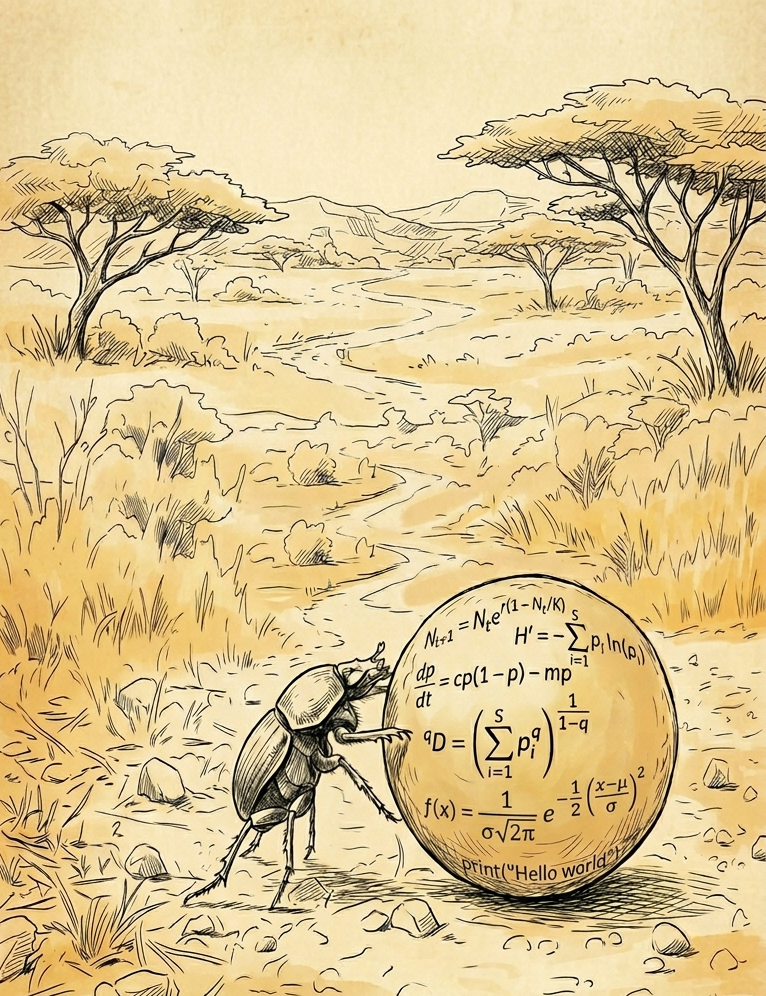
\includegraphics[keepaspectratio]{cover.png}}

\bookmarksetup{startatroot}

\chapter*{Preface}\label{preface}
\addcontentsline{toc}{chapter}{Preface}

\markboth{Preface}{Preface}

This book should not exist. There are already so many free available
materials online. Many universities have materials and open courses
(examples). There are PDF and books available. There are videos on
YouTube, some might be more legitimate than others. I also hope that
there are libraries where you are and you have access to recent
up-to-date physical books\ldots if you are student do not hesitate to
make a request to your advisors and acquaintances, still stay
reasonable. As far as know, foreign researchers are not shy on bringing
knowledge. Just ask!!! And ultimately, I expect that the major part of
what is written here are taught during undergraduate and graduate
courses at your institutions.

So is there a need for this book? Well, I aim and try to address
superficial problems with this book. The first problem is decentralized
information. Maybe there is a book on coding and another book on
statistics. Maybe in some books, the basics are not covered so you need
to look somewhere else. Maybe the levels differ. The first aim to gather
in one place multiple informations, maybe this handbook has an
encyclopedia philosophy. This early realize for instance includes basic
knowledge, with beginner level. basic math vs intermediate math,
descriptive statistics vs statistical inference etc.

Second, focus on intuition and examples. Definition are added for
comprehensive where random because who doesn't like sopopa. this
handbook/encyclopedia is written in a compact form to combine the
intuitive, the formal, and applied perspectives. Each topic will be
divided into 5 parts although there are exceptions . The first part will
provide the intuition for the concept, I will use metaphor etc. This
book is written for Malagasy first so many concepts will be based on
Malagasy culture etc. The second part will focus on the formal
definition which could be Googled, and generally encounter in other
books or teaching materials. This could be boring in the first phase as
it is difficult to define concept in first principle. The third part
will provide a practical side, how to run those things in R. The fourth
part will provide tips and warnings which

Third, this is free book, you can download it from principally my
webpage and probably other pages. Feel free to share it with anyone, use
on whatever you want but this is self-edited book so you should not use
it as a valid citation. As the proverb says, \emph{Saonjo iray lohasa}.
Someone might try to make a business out of it. I am sorry for those who
will pay for it and get scammed.

As a warning, it is worth mentioning that I am no expert in any of the
topics and sections. I am mostly self-taught training in statistics and
programming. There are experts in the field, and I should be the
absolute reference. This book is based on my own experience and the way
how I understand the concept, the way how I code. This is more a
generalist approach to the concept.

About on AI: AI is another blooming stuff and seems like a obvious
approach. In fact, I used AI to help polishing the book. However, I have
a fear of overeliance/dependence and do not recommend reliance on its
usuage without sufficient foundational and criticial thinking about the
topic. Hopefully, this book can provide such basic understanding.

\emph{Preface to version 0.5: beta} Teraka ihany ambatobevohoka. This
has been a long process (mostly thinking) and release this version, yet
leaving the more salient and that . Instead for the following reasons

\begin{itemize}
\item
  Is it the right direction\ldots your feedback is direly needed.
  Finally, don't hesitate to reach out if there is something wrong, you
  will help me greatly. This first release 0.5 is mostly about basic
  topics and still in english. I think it would be useful to have a
  first sense, and depending on time and availability, I will do the
  full release 1.0 in the near future.
\item
  learning the basic is still useful and giving time to do that.
\end{itemize}

And as writing started it became clear that writing in plain text about
what is function in R is actually more challenging that explaining what
is an ANOVA. Utlimately, release the ``first principle first''.

\part{Basic mathematics}

Demistify math. Academic.

Concepts

Math is the foundation of all quantitative methods. And since this is
about quantitative method, it is natural that I start with that. The
existence of this part is written so that we have a basis. You might
even want to skip this, but when you face, notation and concept issues
in later chapter, you can also go back to genesis.

It has become a standard materials for humorists about the uselessness
of math (think about the use of sqrt of 25 or the use of a compas).
Mathphobia is real, and these jokes probably easy the trauma some people
had about that in the past. The goal is not prove that this or find the
limit or analyses is hard, polynomial is not clear or identity
remarkable, application, affine, solve equation, factories,
multiplication, \& addition, go to the basics So, this book is applied
here is to show how useful math is. Where it is applied in the real
world, and more specifically in data analyses.

As said above, most chapters are to support concept introduced later but
I developed things that weak in people, such as operation, notations,
matrix, and graphical representation and representation of few most
useful fonction (such log and exponentional), I will also talk about
derivative, qualitative and quantiative in a math way, and difference
and differential equation. These are I think minimal to with applield
math.

Formalize concepts! We are lost in the formalization.

Crawl before you walk, walk before to run

\chapter{Arithmetic operation}\label{sec-arithmeticMath}

The equation that broke the internet!

Few years ago, there was an intense debate on several social media
platforms about a simple calculation

8 ÷ 2 (2 + 2) = ?

One camp would argue that the answer is one, the other camp is convinced
that it is sixteen. This is an example viral: simple enough to engage
everyone, two possible answers to create camps and fuel discussion. The
question is mostl likely formulated to confuse. But it is still simple
arithmetic operation that a primary schooler should be able to answer.

So what is the correct answer? Let's review below the basic rules of
arithmetic

\section*{Formal}\label{formal}
\addcontentsline{toc}{section}{Formal}

\markright{Formal}

Quick review of order operation

\begin{itemize}
\item
  Parenthesis has priority. Inner-est to outer-most
\item
  Power over multiplication and division
\item
  Multiplication and division over addition and substraction
\item
  Left to right if equal priority
\end{itemize}

\section*{Examples}\label{examples}
\addcontentsline{toc}{section}{Examples}

\markright{Examples}

\begin{enumerate}
\def\labelenumi{\arabic{enumi}.}
\tightlist
\item
  \(1 + 2 \times 3^4 = 1 + 2 \times 81  = 1 + 162  = 163\)
\item
  \((1 + 2) \times 3^4 \neq 1 + (2 \times 3)^4 \neq (1 + 2 \times 3)^4\)
\item
  \(2^{2^2} = 2^4 = 16\)
\item
  \(\frac{1}{\frac{2}{3}} \neq \frac{\frac{1}{2}}{3}\)
\item
  Unecessary for associativity \((1 + 1) + 1 = 1 + (1 + 1)\) and
  \((1 \times 2) \times 3 = 1 \times (2 \times 3)\)
\item
  Necessary parentheses when non-communtative
  \(1 - 2 + 3 = (1 - 2) + 3 \neq 1 - (2 + 3)\) or
\end{enumerate}

\section*{Tips and warning}\label{tips-and-warning}
\addcontentsline{toc}{section}{Tips and warning}

\markright{Tips and warning}

\begin{itemize}
\tightlist
\item
  Solution to the problem is above \texttt{8\ ÷\ 2\ (2\ +\ 2)}

  \begin{itemize}
  \tightlist
  \item
    re-write to \texttt{8\ ÷\ 2\ x\ (2\ +\ 2)}\$,
  \item
    do parenthese first \texttt{8\ /\ 2\ x\ 2}
  \item
    Equal priority, so go left to right \texttt{4\ x\ 2\ =\ 8}. To
    convince yourself about priority, think of 2 - 2 + 3 (same would you
    do 2 + 3 first).
  \end{itemize}
\item
  Three notations for multiplication \texttt{x}, \texttt{.} and nothing
  \texttt{} as in \texttt{a\ b}. While the latter makes compact it is
  also a source of confusion. One classic error in coding is forgetting
  to explicitly add a \href{@sec-matrixOperationCoding}{multiplication
  symbol}
\item
  There are also three notations for division \texttt{÷}, \texttt{/} and
  \(\frac{}{}\). The latter can clarify priority and avoid usage of
  parentheses. Unfortunately, that symbol is not available in R
  language. \(\frac{1}{2} \times 3 = \neq \frac{1}{2 \times 3}\) instead
  of \(1/2 \times 3\)
\item
  Just add parenthesis when in doubt even it might be unnecessary--this
  can be important especially when coding.
\item
  The rule of power over multiplication and multiplication over addition
  should be natural. In fact, multiplication by definition is a
  generalization of addition: \(2 + 2 + 2 + 2 = 2 \times 4\). Thus if
  you reverse and \(2 * 4 + 3 = 2 + 2 + 2 + 2 + 3\).
\item
  The same applies to power \(2 ^ 3 = 2 \times 2 \times 2\). This if you
  revers \(2^3 \times 3 = 2 \times 2 \times 2 \times 3\) and
  \(2^3 + 3 = 2 \times 2 \times 2 + 3\)
\end{itemize}

~

\chapter{Greek letters}\label{sec-greek}

The one like the fish.

Once, a colleague gave a lecture on Lotka-Volterra equation to
undergraduate students in the biology department. When a student asked:
``what is alpha?'', she spent a few minutes explaining what alpha
represented until another student interjected and said: ``it is the one
like the fish''. It was a wake up call that understanding greek letter
is a problem. And to the majority it is the case, so let's clear that
out.

This is unfamiliar \((\zeta  + \xi)^2 = \zeta^2 + \xi^2 + 2\zeta\xi\),
yet the \emph{identité remarquable} \((a + b) ^ 2 = a^2 + b^2 + 2ab\)

Roman notation is also impossible to do \(XIII + IX = XXII\), while this
\(13 + 9 = 22\) is trivial

A major barrier to is inability to go past beyond notation. While in the
right context, using roman number feels normal when siting section in
the bible. First because we are used to it, but second because we
understand the specific choice (separete section and verse).

So as every notation: greek letter are used with convience (not a
necessity), and as with roman numbers, habits, basic comprehension are
elements to be comfortable with them

\section*{Formal}\label{formal-1}
\addcontentsline{toc}{section}{Formal}

\markright{Formal}

Here is dictionary of the greek alphabet in upper and lower case, the
latin equivalent, and how to call them

{\def\LTcaptype{none} % do not increment counter
\begin{longtable}[]{@{}llll@{}}
\toprule\noalign{}
Lower Case & Upper Case & Latin Equivalent & Name \\
\midrule\noalign{}
\endhead
\bottomrule\noalign{}
\endlastfoot
\(\alpha\) & \(A\) & a & Alpha \\
\(\beta\) & \(B\) & b & Beta \\
\(\gamma\) & \(\Gamma\) & g & Gamma \\
\(\delta\) & \(\Delta\) & d & Delta \\
\(\epsilon\) & \(E\) & e & Epsilon \\
\(\zeta\) & \(Z\) & z & Zeta \\
\(\eta\) & \(H\) & e & Eta \\
\(\theta\) & \(\Theta\) & th & Theta \\
\(\iota\) & \(I\) & i & Iota \\
\(\kappa\) & \(K\) & k & Kappa \\
\(\lambda\) & \(\Lambda\) & l & Lambda \\
\(\mu\) & \(M\) & m & Mu \\
\(\nu\) & \(N\) & n & Nu \\
\(\xi\) & \(\Xi\) & x & Xi \\
\(\omicron\) & \(O\) & o & Omicron \\
\(\pi\) & \(\Pi\) & p & Pi \\
\(\rho\) & \(R\) & r & Rho \\
\(\sigma\) & \(\Sigma\) & s & Sigma \\
\(\tau\) & \(T\) & t & Tau \\
\(\upsilon\) & \(\Upsilon\) & y & Upsilon \\
\(\phi\) & \(\Phi\) & ph & Phi \\
\(\chi\) & \(X\) & ch & Chi \\
\(\psi\) & \(\Psi\) & ps & Psi \\
\(\omega\) & \(\Omega\) & o & Omega \\
\end{longtable}
}

\section*{Examples}\label{examples-1}
\addcontentsline{toc}{section}{Examples}

\markright{Examples}

\begin{itemize}
\tightlist
\item
  ``I am \(\alpha\) and \(\Omega\)'', probably the most famous use of
  greek letters to mean beginning and the end.
\item
  \(\pi\) represents the number 3.14 etc We could also think that
  \(\pi\) is the ratio between the circumference and diameter. So it
  represents a constant
\item
  \(\sigma\) is used as the parameter for standard deviation for a
  normal distribution. The variance is \(\sigma^2\).
\item
  \(\Sigma\) and \(\Pi\) are used for shortcut summation and product see
  Chapter~\ref{sec-sum}.
\item
  \(\Omega\) is usually used to represent a set, but can mean something
  else in physics.
\item
  \(\zeta\) is one of famous equation that mathematicians are hoping to
  solove
\item
  \(\epsilon\) and \(\omicron\) \(\iota\) etc are something small
\end{itemize}

\section*{Tips and warning}\label{tips-and-warning-1}
\addcontentsline{toc}{section}{Tips and warning}

\markright{Tips and warning}

\begin{itemize}
\tightlist
\item
  Greek letters are used to show difference.

  \begin{itemize}
  \tightlist
  \item
    In statistics, difference between true value (\(\sigma\)) for
    standard deviation of the \href{@sec-population}{population}
    vs.~\(s\) for estimated value from the sample.
  \item
    In mathematics: greek could represend parameter while represent
    variable \(\mu\) is for mortallity instead x, y, for variable and t
    for time.
  \end{itemize}
\item
  Use of greek letter for paremeters in probability: \(N(\mu, \sigma)\)
  or Poisson(\(\lambda\))
\item
  Use of greek letters for covid variants.
\item
  Latin browed letters from Greek. When the romans picked the letter,
  some of them were dropped because romans did not need them (like phi)
  or modified them, Delta, Lambda and sigma. while some kept the same.
\end{itemize}

\chapter{Discrete and continuous number}\label{sec-discrete_continuous}

To count or to measure.

The title of that chapter should be natural numbers \(\mathbb{N}\) and
real numbers \(\mathbb{R}\). Those are sets that everyone are familiar
with. Because the set of natural numbers is a subset of real numbers,
one can basically use real number and ignore the set of natural numbers.

So why such a title and why the distinction? The answer to the first
question is because this book is about applied mathematics and more an
emphasis about the properties than nomenclature. In other words, natural
numbers has the properties of discrete, while real numbers is a
continuous set. The difference between discrete and continuous will
appear in the statistics parts (discrete and continuous variables
Chapter~\ref{sec-quantitative-variable}) and again implemented
differently in \href{@sec-numeric}{programming language}.

\section*{Formal}\label{formal-2}
\addcontentsline{toc}{section}{Formal}

\markright{Formal}

The formal definition is useless in the purpose of this book (unless you
want to learn about topology). It could describe in the following, a
discrete discrete set, every number is isolated. In contrast, in a
continuous, any number has a neighbor. And this is true no matter how
close one looks. That is why a continuous number (real number) is
represented by a continuous line where as natural number should be
points.

\section*{Examples}\label{examples-2}
\addcontentsline{toc}{section}{Examples}

\markright{Examples}

\begin{itemize}
\item
  World of discrete numbers: Odd (2, 4, 6, 8 etc) and even (3, 5, 7, 9
  etc.), prime numbers (3, 5, 7, 11, etc), and also the negative mirror.
\item
  World of continuous numbers: \(\pi = 3.14\ldots\), \(e = 2.71\ldots\),
  \(\sqrt(2)\) and the fractions
\end{itemize}

\section*{Tips and warnings}\label{tips-and-warnings}
\addcontentsline{toc}{section}{Tips and warnings}

\markright{Tips and warnings}

\begin{itemize}
\tightlist
\item
  Semantic: whole number, natural number, integer while the later
  includes mirror negative
\item
  Discrete number is mostly used for counting and indexing (e.g.~in
  summation and product Chapter~\ref{sec-sum})
\item
  Tools to are fundamentaly different.

  \begin{itemize}
  \tightlist
  \item
    For instance, using\href{@sec-difference}{difference equation} to
    model when time is discrete and
    \href{@sec-differential}{differential equation} when time is
    continuous.
  \item
    In probabilites, a sum is used to compute the mean if the variable
    is discrete, an integral is used if the variable is continuous
  \end{itemize}
\end{itemize}

\chapter{Sum and product and dummy variable}\label{sec-sum}

Acronyms in mathematics!

When talking with people at the ministry in conservation , they are
found of acronyms, PAEP etc. While they are fluent with that, they often
do not realize that outsiders have no idea of what they are talking
about.

Conversely, when mathematicians are using acronyms (symbols) to
condense\ldots it is universally unaccessible. Mathematicians (too) are
found of creating new symbols to condense a repeated expression.
Multiplication is a notation used so not repeat addition. So 2 + 2 + 2 =
3 * 2. Another example is
\texttt{n!\ =\ 1\ x\ 2\ x\ 3\ x\ ...\ (n\ -\ 1)\ x\ n}. And the list is
long.

Two fundamental notation this scare ecologits are the summation notation
(\(\Sigma\)) and the product \(\Pi\). Maybe because it is a greek
notation but also because it is often followed by more expressions.

Following the greek, one observation is that \(\Sigma\) is the greek of
equivalent of capital S (short of sum), and \(\Pi\) is the equivalent of
capital P (short for product). They are used when there is a repeating
patterns in the expression that one wants to add or multiplity.

\section*{Formal}\label{formal-3}
\addcontentsline{toc}{section}{Formal}

\markright{Formal}

Here is one general form of a summation:

\[
\sum_{i = n_0}^{n_f} a_i = a_{n_0} + a_{n_0 + 1} + \cdots + a_{n_f - 1} + a_{n_f}
\]

Let's break down (always a good idea when looking at math notation).

\begin{itemize}
\tightlist
\item
  \(\sum\) is summation symbol
\item
  \(i\) is a dummy variable and is found under the summation and in the
  expression, here \(a_i\)
\item
  \(n_0\) represent the first expression in the summation. i.e, replace
  \(i\) in \(a_i\) by \(a_{n_0}\)
\item
  \(n_f\) is the last expression which ends the summation
\end{itemize}

For the product, just replace \(+\) by \(\times\)
\[\prod_{i = n_0}^{n_f} a_i = a_{n_0} \times a_{n_0 + 1} \times \cdots \times a_n \]

The hidden/implied part is that one start by \(n_0\), then add 1 until
the dummy variable is equal to \(n_f\). It is a sequence of discrete
numbers \([ n_0, \ldots, n_f ]\).

\section*{Examples}\label{examples-3}
\addcontentsline{toc}{section}{Examples}

\markright{Examples}

\begin{itemize}
\item
  Identifying where the dummy variable is in the expression \[
    \sum_{i = n_0}^{n_f} i^a = {n_0}^a + \cdots + {n_f}^a
  \]
\item
  Defining a argument of a function instead of index \[
    \sum_{i = n_0}^{n_f} f(i) = f(n_0) + \cdots + f(n_f)
  \]
\end{itemize}

Concrete example OF summation -
\[\sum_{i=0}^7 i = 0 + 1 + 2 + \cdots + 6 + 7\]

\begin{itemize}
\tightlist
\item
  \[ \sum_{i=3}^7 i^2 =  3^2 + 4^2 + \cdots + 6^2 + 7^2 \]
\item
  \[
     \sum_{i=0}^7 sin(\frac{1}{i+1}) = sin(\frac{1}{1+ 0}) + sin   (\frac{1}{ 1+ 1}) + \cdots + sin(\frac{1}{7+1})
  \]
\end{itemize}

Same example but replacing \(\sum\) with \(\prod\).

\begin{itemize}
\item
  \(\prod_{i = 1}^n i = 1 \times 2 \times 3 \times \cdots \times (n-1) \times n = n!\)
  because it is used so often than it warrants another notation
\item
  \(\prod_{i=3}^7 i^2 = 3^2 \times 4^2 \times  \cdots \times 6^2 \times 7^2\)
\item
  The summation can be infinite
  \(\Sigma_{i = 0}^\infty \frac{1}{i!} = \frac{1}{0!} + \frac{1}{1!} +\frac{1}{2!} + \cdots = 2.71\ldots = e\)
\end{itemize}

\section*{Tips and warning}\label{tips-and-warning-2}
\addcontentsline{toc}{section}{Tips and warning}

\markright{Tips and warning}

\begin{itemize}
\item
  Whenever facing a complicated expression, break it down piece by
  piece.
\item
  Sometimes it helps to take a pen and paper and try with the first few
  terms
\item
  Dummy variable: the i is dummy and can be replaced by anything \[
    \sum_{i = 1}^n \frac{1}{i!} = \sum_{j = 1}^n \frac{1}{j!} = \Sigma_{k = 1}^n \frac{1}{k!}
   \]
\item
  Better to denote the dummy by a single letter.
\item
  The sequence should also be defined by a set, in that case the set
  should be defined explicitly. \(\Omega = [2, 9, 21, 25]\), then \[
   \sum_{\omega \in \Omega} a_\omega = a_2 + a_9 + a_{21} + a_{25}
  \]
\item
  There could be double or more summation. First start with the inner
  summation while keeping the outer fixed. Then change the outer. \[
    \sum_{j \in \{a, b\}} \sum_{i=1}^3 i ^ j =
   ( 1 ^ a + 2 ^ a + 3 ^ a )+ (1 ^ b  + 2 ^ b + 3 ^ b)
    \].
\end{itemize}

\chapter{Matrix}\label{sec-matrixMath}

Not the movie by Keanu Reaves

While french can be creative when translating movie titles, they kept
Matrix the movie by Keanue Reaves. With the popularity of the series,
when talking about matrix. The frustration is familiar to malagasy
people when people first think about the animated series, lions and
zebra, before their island. Matrix, a mathematical object, existed well
before the movie series.

A matrix could simply be a way fo storing numbers.

Rabe, Rakoto, Sanda, Dora when to market and here are what they bought
Rabe bought 6 bananas, 3 toko strawberries, and 0.5 kapoaka of
voatsinefy. Rakoto bought 3 bananas, 1 toko of strawberries, no
voatsinefy Sanda bought only 10 toko of strawberries. Finally, Dora
bought 1 banana and 2 kapoaka of vaotsinefy.

This information is arrange in a matrix, each row represents a
purchaser, and a column a fruit \[
\begin{pmatrix}
    6 & 3 & 0.5 \\
    3 & 1 & 0 \\
    0 & 10 & 0 \\
    1 & 0 & 2
\end{pmatrix}
\]

Alternatively, we can structure the data \[
\begin{pmatrix}
6 & 3 & 0 & 1 \\
3 & 1 & 10 & 0 \\
0.5 & 0 & 0 & 2
\end{pmatrix}
\]

The conversion from the first matrix to the second one is called
transposing.

\section*{Formal}\label{formal-4}
\addcontentsline{toc}{section}{Formal}

\markright{Formal}

An \(m \times n\) matrix is a rectangular array of elements in a set
\(\Omega\) having m rows and n columns. It is denoted as:

\[
A =
\begin{pmatrix}
    a_{11} & a_{12} & \dots & a_{1n} \\
    a_{21} & a_{22} & \dots & a_{2n} \\
    \vdots & \vdots & & \vdots \\
    a_{m1} & a_{m2} & \dots & a_{mn}
\end{pmatrix}
\]

where the element \$a\_\{i,j\} \in \Omega \$ denotes the entry in the
ith row and jth column of A. The domain of the row index i is
\{1,2,\ldots,m\} and the domain of the column index j is
\{1,2,\ldots,n\}. \(\Omega\) could be natural or real number or anything
else.

In mathematics, a vector is special case of matrix, consisting of with
one column.

\section*{Examples}\label{examples-4}
\addcontentsline{toc}{section}{Examples}

\markright{Examples}

\begin{itemize}
\tightlist
\item
  As square matrix is with the same number of row and column
\end{itemize}

\[
\begin{pmatrix}
6 & 3 & 0 \\
3 & 1 & 10 \\
0.5 & 0 & 0
\end{pmatrix}
\]

\begin{itemize}
\item
  A diagonal matrix has all element of the diagonal equals to 0, it is
  often noted diag() \[
  \begin{pmatrix}
  a & 0 & 0 \\
  0 & b & 0 \\
  0 & 0 & c
  \end{pmatrix}
  \]
\item
  A matrix can be symmetric where the values are the same the diagonal,
  ie \(a_{i,j} = a_{j,i}\) \[
  \begin{pmatrix}
  a & 1 & x \\
  1 & b & -1 \\
  x & -1 & c
  \end{pmatrix}
  \]
\end{itemize}

\section*{Tips and warning}\label{tips-and-warning-3}
\addcontentsline{toc}{section}{Tips and warning}

\markright{Tips and warning}

\begin{itemize}
\tightlist
\item
  Semantic: element, entry,
\item
  A matrix is often denoted by a capital letter, sometimes in bold to
  differentiate from value which are mostly lower case.
\item
  A community matrix for ecologist have the number of species per site
\item
  A distance matrix is a square and symmetric matrix computed after say
  community matrix. Each element is pairwise distance between two sites.
  Since distance between site A and site B is the same as the distance
  between site B and site A. The element on the diagonal is the distance
  between the same site and could be 0 or 1 depending on the distance
  represent similarity or dissimilarity.
\item
  From a mathematical matrix, a column matrix is different than a row
  matrix (1 x n) is not the same as (n x 1) although one can transpose
  it.
\item
  Matrix is more than a rectangle storing data, it is the foundation of
  linear algebra\ldots and sometimes have magical properties. Maybe in
  future chapters
\item
  A \href{@sec-dataframe}{data frame} is also a rectangular object
  mostly used in data-science. The columns could be a different type
  (numbers, text, etc.). There is no equivalent of data frame in
  mathematics.
\item
  The huge field of linear algebra in mathematics is essentially
  understand the properties of matrix.
\end{itemize}

\chapter{Matrix operation}\label{sec-matrixOperationMath}

Andry + Fenitra = Tolotra

A reccurent theme in this first part of the book is that symbols and
terms are the same but have different meaning. A variable is used in
mathematics, in \href{@sec-variable}{statistics}, or a
\href{@sec-functionMath}{function} in mathematics and a
\href{@sec-functionCoding}{function} in programming. There are
similarities but also nuanced meanings.

Above is an example of using mathematical notations (addition and
equality) which differ from strict mathematical definition. Yet, they
actually have a meaning, maybe not as rigorous as in mathematics.

In the previous a matrix is new kind of object, and it is worth defining
what kind of operation can be done. The general idea is to generalize
some of the arithmetic operation. What does it mean adding two matrices:
Matrix 1 + Matrix 2 or multiplying two matrices Matrix 1 x matrix 2.

This chapter focuses element wise operation.

Let's reuse the example in \href{@sec-matrixMath}{this chapter}

\[
A =
\begin{pmatrix}
    6 & 3 & 0.5 \\
    3 & 1 & 0 \\
    0 & 10 & 0 \\
    1 & 0 & 2
\end{pmatrix}
\]

amd multiply with 2

\[
2 \times A =
\begin{pmatrix}
    2 \times 6 & 2 \times 3 & 2 \times 0.5 \\
    2 \times 3 & 2 \times 1 & 2 \times 0 \\
    2 \times 0 & 2 \times 10 & 2 \times 0 \\
    2 \times 1 & 2 \times 0 & 2 \times 2
\end{pmatrix}
\]

This element-wise work (well-defined) when we combine a matrix with
scalar or matrix of same dimension wi, the element-wise operation is
mostly arithemetic operation for each element of the grid. All the
propreties in traditional arithmetic operation with numbers naturally
apply.

\section*{Formal}\label{formal-5}
\addcontentsline{toc}{section}{Formal}

\markright{Formal}

Consider a number \(x\), a matrix \(A = \{a_{i,j}\}\) and
\(B = \{b_{i,j}\}\) of dimensions \(m\) and \(n\).

\textbf{The scalar operation are}

\begin{itemize}
\tightlist
\item
  Addition a scalar \(x + A =  \{x + a_{i,j}\}\) for all i and j
\item
  Multiplication a scalar \(x \times A =  \{x \times a_{i,j}\}\) for all
  i and j
\item
  Subtract a scalar \(x - A =  \{x - a_{i,j}\}\) for all i and j
\item
  Divide a scalar \$ x / A = \{x / a\_\{i,j\}\}\$ for all i and j
\end{itemize}

It should be obvious that \(A + x\), \(A - x\), \(A \times x\) and
\(A / x\) are defined in the same manner

\textbf{Two matrices have the same dimensions}

\begin{itemize}
\tightlist
\item
  Addition a scalar \(A  + B =  \{a_{i,j} + b_{i,j}\}\) for all i and j
\item
  Subtract a scalar \$ A - B = \{a\_\{i,j\} - b\_\{i,j\}\}\$ for all i
  and j
\item
  Divide a scalar \$ x / A = \{x / a\_\{i,j\}\}\$ for all i and j
\end{itemize}

For a multiplication, a special notation is used
\(A  \circ B =  \{a_{i,j} \times b_{i,j}\}\) and is called a Hadamard
product.

The equivalent division, called Hadamard quotient, also exists and is
noted: \(A  \circ B^{-1} =  \{\frac{a_{i,j}}{b_{i,j}}\}\)

\section*{Examples}\label{examples-5}
\addcontentsline{toc}{section}{Examples}

\markright{Examples}

\begin{itemize}
\item
  With the example above adding 1 but in practice it does not have
  trivial intepretation \[
  A + 1 =
  \begin{pmatrix}
    6 + 1 & 3 + 1 & 0.5 + 1\\
    3 + 1 & 1 + 1 & 0 + 1 \\
    0 + 1 & 10 + 1 & 0 + 1\\
    1 + 1 & 0 + 1 & 2 + 1
  \end{pmatrix}
  \]
\item
  Notice that multiplying the matrix by 2 above is the same of having
  the same purchase.
\item
  Assume we want to conver the matrix A into kg. Assume 1 banana is 0.2
  kg, one toko is 0.5 kg, and one kapoka is 0.3 kg. Constructing a
  matrix B
\end{itemize}

\[
B =
\begin{pmatrix}
    0.2 & 0.5 & 0.3 \\
    0.2 & 0.5 & 0.3 \\
    0.2 & 0.5 & 0.3 \\
    0.2 & 0.5 & 0.3
\end{pmatrix}
\] The conversion is done by doing a Hadamard product of A and b

\$\$ A \circ B = A =

\begin{pmatrix}
    6 & 3 & 0.5 \\
    3 & 1 & 0 \\
    0 & 10 & 0 \\
    1 & 0 & 2
\end{pmatrix}
\circ
\begin{pmatrix}
    0.2 & 0.5 & 0.3 \\
    0.2 & 0.5 & 0.3 \\
    0.2 & 0.5 & 0.3 \\
    0.2 & 0.5 & 0.3
\end{pmatrix}

=

\begin{pmatrix}
    6 \times 0.2 & 3 \times 0.5 & 0.5 \times 0.3 \\
    3 \times 0.2 & 1 \times 0.5 & 0 \times 0.3 \\
    0 \times 0.2 & 10 \times 0.5 & 0 \times 0.3 \\
    1 \times 0.2 & 0 \times 0.5 & 2 \times 0.3
\end{pmatrix}

\$\$

\section*{Tips and warning}\label{tips-and-warning-4}
\addcontentsline{toc}{section}{Tips and warning}

\markright{Tips and warning}

\begin{itemize}
\tightlist
\item
  Mathematics well defined.
\item
  Because matrix in data, these operation are and the goal is to find
  how they are implement in R. For instance, the \(\circ\) in Hadamard
  product is not a standard character so a different symbol might be
  used.
\item
  There are other matrix product (e.g.~Kronecker), leave at your
  discretion for now, we might need them later and will be defined
\item
  You might run into issues, when you apply them in coding might not be
  as straighforwad.
\item
  Careful with division as
\item
  Element-wise power could also be defined in the same way.
\end{itemize}

\chapter{Matrix multiplication}\label{sec-matrixMultiplicationMath}

Asio facture azafady!

Wasn't matrix multiplication defined in the previous
\href{@sec-matrixOperationCoding}{chapter}? Yes but it is specifically
called Hadamard product or element-wise multiplication. But also as
stated in the first sentence of that chapter, same terms and same
symbols are used and meaning depends on the context. Here, another
multiplication, but this is \textbf{the most used and useful matrix
multiplication}.

Matrix multiplication is something that we encounter all the time.
Consider again the purchase matrix earlier. Rabe bought 6 bananas, 3
toko strawberries, and 0.5 kapoaka of voatsinefy. Rakoto bought 3
bananas, 1 toko of strawberries, no voatsinefy. Sanda bought 10 toko of
strawberries. Finally, Dora bought 1 banana and 2 kapoaka of vaotsinefy.

\[
A = \begin{pmatrix}
    6 & 3 & 0.5 \\
    3 & 1 & 0 \\
    0 & 10 & 0 \\
    1 & 0 & 2 \\
\end{pmatrix}
\]

Now assume one banana is 500 Ar, a toko of strawberries is 1000, and a
kapoaka of voatsinefy is 2000 Ar. To get how much Rabe paid, we do

\(500 \times 6 + 1000 \times 3 + 2000 \times 0.5 = 7000\), for Rakoto
\(500 \times 3 + 1000 \times 1 + 2000 \times 0 = 2500\), for Rabe etc.
This is a natural calculation when get ask for a check or a receipt.
This is process is condensed with a matrix multiplication

\[
A \cdot P
\] where \[
P =
\begin{pmatrix}
    500 \\
    1000 \\
    2000
\end{pmatrix}
\]

One important condition is that the multiplication makes sense only the
the number of column in the first matrix is the same as the number of
rows in the second matrix--otherwise there is no pairs to multiply.

\section*{Formal}\label{formal-6}
\addcontentsline{toc}{section}{Formal}

\markright{Formal}

Matrix multiplication is an operation that takes two matrices and
produces a single new matrix by taking the dot product of rows from the
first matrix and columns from the second.

For matrix multiplication to be possible, the number of columns in the
first matrix must equal the number of rows in the second matrix.

If Matrix \(A\) has dimensions \(m \times n\) and Matrix \(B\) has
dimensions \(n \times p\):

Their product \(C = A \cdot B\) is a matrix of dimension \(m \times p\).
Each entry \(c_{i,j}\) in the product matrix \(C\) represents the dot
product of the \emph{\(i\)-th row of \(A\)} and the \emph{\(j\)-th
column of \(B\)}:

\[c_{i,j} = \sum_{k=1}^{n} a_{i,k} \cdot b_{k,j} = a_{i,1}b_{1,j} + a_{i,2}b_{2,j} + \dots + a_{i,n}b_{n,j}\]
NOTE: A good example to practice \href{@sec-sum}{summation notation}.

\section*{Examples}\label{examples-6}
\addcontentsline{toc}{section}{Examples}

\markright{Examples}

\begin{itemize}
\tightlist
\item
  The price of fruit differ among markets, in another market, the price
  of the fruits were and we combine both price in matrix with two
  columns \[
  Q =
  \begin{pmatrix}
    500 & 600 \\
    1000  & 800 \\
    2000 & 2500
  \end{pmatrix}
  \]
\end{itemize}

The product \$ A \cdot Q\$ will give the total for each market
\[ A \cdot Q
\begin{pmatrix}
    6 & 3 & 0.5 \\
    3 & 1 & 0 \\
    0 & 10 & 0 \\
    1 & 0 & 2 \\
\end{pmatrix}
\cdot
\begin{pmatrix}
    500 & 600 \\
    1000  & 800 \\
    2000 & 2500
\end{pmatrix} =
\begin{pmatrix}
  7000 & 7250 \\
  2500 & 2600 \\
  10000 & 8000 \\
  4500 & 5600
\end{pmatrix}
\]

\begin{itemize}
\item
  Multiplication with identity matrix \[ A \cdot ID
  \begin{pmatrix}
    6 & 3 & 0.5 \\
    3 & 1 & 0 \\
    0 & 10 & 0 \\
    1 & 0 & 2
  \end{pmatrix}
  \cdot
  \begin{pmatrix}
    1 & 0 & 0 \\
    0 & 1 & 0 \\
    0 & 0 & 1
  \end{pmatrix}
  =
  \begin{pmatrix}
    6 & 3 & 0.5 \\
    3 & 1 & 0 \\
    0 & 10 & 0 \\
    1 & 0 & 2
  \end{pmatrix}
  \] This is like multiplying by one in the arithmetic operation.
\item
  Projecting the number of juvenile and adult of an annual plant with a
  Leslie matrix (\(L\)). Assume \(40\%\) of juvenile survives to
  adulthood after one year, and adult only lives for one year.Juvenile
  does not produce offspring. An adult produces 2 juveniles in one year.
  We can turn that information into a matrix called Leslie matrix
\end{itemize}

\[
L =
\begin{pmatrix}
0 & 2.0 \\
0.4 & 0
\end{pmatrix}
\]

If the initial population vector is \(N_{\text{now}} =
\begin{pmatrix}
  100 \text{ (juveniles)} \\
  50 \text{ (adults)}
\end{pmatrix}\),

The population at time one year after is
(\(N_\text{next} = L \cdot N_{\text{now}}\)) is calculated via matrix
multiplication:

\[
N_\text{next} =
\begin{pmatrix}
    0 & 2.0 \\
    0.4 & 0
\end{pmatrix}
\cdot
\begin{pmatrix}
100 \\
50
\end{pmatrix} =
\begin{pmatrix}
(0 \cdot 100) + (2.0 \cdot 50) \\
(0.4 \cdot 100) + (0 \cdot 50)
\end{pmatrix}
=
\begin{pmatrix}
100 \text{ juveniles} \\
40 \text{ adults}
\end{pmatrix}
\]

\begin{itemize}
\item
  Biomass (\(\text{g/m}^2\)) in as a function of soil nitrogen (\(\%\))
  and Annual Rainfall (\(\text{m}\)) at 4 sites. In this specific
  example assume we know the effect of each of the parameter on plant
  biomass which the coefficients (\(\beta\)):
\item
  \textbf{\(\beta_0 = 100\):} Baseline biomass
\item
  \textbf{\(\beta_1 = 150\):} \(+150\text{ g/m}^2\) per \(1\%\) nitrogen
\item
  \textbf{\(\beta_2 = 80\):} \(+80\text{ g/m}^2\) per \(1\text{ m}\)
  rainfall
\end{itemize}

The design matrix for each site is

\begin{itemize}
\tightlist
\item
  Site 1 (Arid / Low Nitrogen): 0.2\% Nitrogen, 0.8~m Rainfall.
\item
  Site 2 (Warm Grassland): 0.5\% Nitrogen, 0.6~m Rainfall.
\item
  Site 3 (Wet / Low Nitrogen): 0.1\% Nitrogen, 1.5~m Rainfall.
\item
  Site 4 (Fertile Woodland): 0.4\% Nitrogen, 1.2~m Rainfall.
\end{itemize}

\[
\begin{matrix}
    \text{Site 1} \\
    \text{Site 2} \\
    \text{Site 3} \\
    \text{Site 4}
\end{matrix}
\begin{pmatrix}
  1 & 0.2 & 0.8 \\
  1 & 0.5 & 0.6 \\
  1 & 0.1 & 1.5 \\
  1 & 0.4 & 1.2
\end{pmatrix}
\cdot
\begin{pmatrix}
  100 \\
  150 \\
  80
\end{pmatrix}
 =
\begin{pmatrix}
  194 \\
  223 \\
  235 \\
  256
\end{pmatrix}
\]

This is an illustration, in practice we know the biomass, and the design
matrix (we measured them). The goal is generally to estimate the
coefficient \(\beta\).

\section*{Tips and warning}\label{tips-and-warning-5}
\addcontentsline{toc}{section}{Tips and warning}

\markright{Tips and warning}

\begin{itemize}
\tightlist
\item
  There is no division, when the inverse however exist, we can multiply
  by the inverse.
\item
  Inverse of a matrix Think about a null matrix, there is no second
  matrix to multiply with
\item
  A linear model is essentially a A x + b = y is a matrix multiplication
  A times
\item
  It is essential to understand that multiplication, and one can do it
  by hand, however, R programming can do that with almost not cost
  (Chapter~\ref{sec-matrixOperationCoding}).
\end{itemize}

More mathematica properties

\begin{itemize}
\tightlist
\item
  \textbf{Non-Commutative:} In general, \(A \cdot B \neq B \cdot A\).
  The order of multiplication matters.
\item
  \textbf{Associative:} \((A \cdot B) \cdot C = A \cdot (B \cdot C)\)
\item
  \textbf{Distributive:} \(A \cdot (B + C) = A \cdot B + A \cdot C\)
\end{itemize}

\chapter{Functions}\label{sec-functionMath}

f(x) = y

Hearing a function is traumatizing. Many think of ``domaine de
définition, dérivé, étude des signes, et tableau de variation etc.'' To
a certain extent, many has lost what is the true meaning of a function
and its incredible use.

What matters the most is that mathematical ``formalization'' of a
function. 1- formalization, 2- significance, and 3- the geometric. The
geometric aspect will be elaborated in the next
\href{@sec-function_viz}{chapter}. Formalization is below. But in short,
a function is not only defined by f(x) but also the source set (domain)
i.e.~what are the different choices for x, and the target set (codomain)
i.e.~what are the outcomes are supposed to be. These concepts will
reappear also in statistics (Chapter~\ref{sec-population},
Chapter~\ref{sec-variable}) as well as in computer programming
(Chapter~\ref{sec-functionCoding}) when the domain and codomain are not
necessarily numbers.

A second point: significance is what brings function to life. This is
mostly in acamdemic \(f(x) = \frac{e^x}{sin(x) + x^2}\). In this applied
book, the intent is on the practical side and the goal is to find a
function that relates two variables. For instance, change in average
income as a function of age, rise in temperature as a function of CO2
emission, number of species as a function of forest size etc. While we
loath the math expression, we will be thrilled if we find the expression
that link the so we can choose which value to reach a desire outcome.
Because it then allows us to predict or control the outcome. It's life
control to obtain a avoid certain outcome.

\section*{Formal}\label{formal-7}
\addcontentsline{toc}{section}{Formal}

\markright{Formal}

A function f is a rule that assigns to each element x in a set D exactly
one element, called f(x), in a set E. The set D is called the domain of
the function. The number f(x) is the value of f at x and is read `f of
x'. The range of f is the set of all possible values of f(x) as x varies
throughout the domain, that is,

\(\text{Range} = \{f(x) \mid x \in D\}\)

In the classic academic, D and E are real numbers, or N to R. The symbol
that represents an arbitrary number in the domain of a function f is
called an independent variable. The symbol that represents a number in
the range of f is called a dependent variable.

This can be generalized, the domain x could multidimensional R x R as
well as the output.

\section*{Examples}\label{examples-7}
\addcontentsline{toc}{section}{Examples}

\markright{Examples}

\begin{itemize}
\tightlist
\item
  y = ax + b, is what is called a linear function, because it draws a
  line. x is the independent variable and y is the dependent variable.
\item
  y = x\^{}2, if think about x as a positiive number, the function
  mostly computes the area of
\item
  The probability density function of the normal distribution is a
  function that maps a real number x to the probability density at that
  point. The function is defined as:
  \[f(x) = \frac{1}{\sigma \sqrt{2\pi}} e^{-\frac{(x - \mu)^2}{2\sigma^2}}\]
\item
  \(F(m_1, m_2, d) = \frac{m_1 \times m_2}{d^2}\) is a function of three
  variables that shows the attraction between two object of mass \(m_1\)
  and \(m_2\) and the distance between the two objects. Notice that it
  only makes sense (in the applied sense) if the R x R X R all are
  well-define especially the units.
\end{itemize}

\section*{Tips and warning}\label{tips-and-warning-6}
\addcontentsline{toc}{section}{Tips and warning}

\markright{Tips and warning}

\begin{itemize}
\item
  Semantic: independent variable, input, covariates, x which is also the
  common notation x. Argument, parameter
\item
  Semantic: dependent variable, output, response variable, y, most
  commonly denoted as y.
\item
  Semantic: function, application, map
\item
  The mathematical function is often denoted as f, g, h because they are
  meant to be symbolic too.
\item
  Implicit f(x, y) = 0, x\^{}2 + y\^{}2 = 0
\item
  Multiple variable
\item
  Find a function based on graphical point (fitting) (statistical) and
  (dynamical) sense find a function that recreates a phenomenon.
\item
  Elementary function:

  \begin{itemize}
  \tightlist
  \item
    Algebraic functions: these are functions that are constructed on the
    arithmetic operation and includes polynomical and quotient function.
    The have those that we can calculate by hand.
  \item
    Transendental functions: trigonometric, hyperbolic, and the
    exponential and logarithmic functions.
  \end{itemize}
\item
  Non elementary: Functions Gamma Bessel Lambert, solution of equation
  but can't expressed on elementary function. In many cases, we are not
  concerned with closed form, more how it looks like and the ultimate is
  the geometric form.
\end{itemize}

\chapter{Function and graphics}\label{sec-functionViz}

Ikotozafy ihany no Alexis!

In the math test at in the baccalaureat, the most points goes into the
section problem: this is calculus problem, a function is given at the
begining, then a series of questions like domaine def, studying
derivative, etc. which culminates with drawing a plot of that function.
The problem is that we are given a function and then asked to draw the
figure. But this is not really a problem, I can just put the function in
a program and I get the graph!

Arguably, the problem is reading and interpreting a graph, by extent
strugle to read scientific figures. Here is where the geometric
propreties the analytical propreties.

Add figure here.

\section*{Formal}\label{formal-8}
\addcontentsline{toc}{section}{Formal}

\markright{Formal}

Add definition of a figure. We focus on real valued function

For simplicity, we look at X and Y as real number. See for more details.
To graphically present a function, we need a few things x axis to
represent the value, we need a scale on that x axis. y axis to represent
the The angle between x and y axis The curve is just how y vary as we
continuously change x

\section*{Examples}\label{examples-8}
\addcontentsline{toc}{section}{Examples}

\markright{Examples}

\begin{itemize}
\item
  Linear function y = a*x + b and
\item
  Exponential and logarithm
\item
  Gaussian
\item
  Logistic
\end{itemize}

\section*{Tips and warnings}\label{tips-and-warnings-1}
\addcontentsline{toc}{section}{Tips and warnings}

\markright{Tips and warnings}

\begin{itemize}
\tightlist
\item
  As in domain, what does x and y represent
\item
  Linear function because it plots a line, pick two points and
\item
  If x is discrete, you cannot just join line.
\item
  Don't rush, project, look at the changes in the axis not the ``line''
\item
  Transforming the response variable
\item
  Transforming
\item
  Cheating
\item
  Just plot and you are good to go.
\end{itemize}

\chapter{Derivative}\label{sec-derivative}

It is just the speed!

Most have learned a set of rules to calculate the derivate of any
functions. The exercices is pattern identification, learning the follow
rules but imbalance at the expense of it's significance. As we can also
plug any function into a program and get the derivative. While Isaac
Netwon was famous as a physicist from its law of gravity and apple, his
is likely as mathematician for ``discovering/defining'' a derivative.

How do you calculate speed? Distance over the time it takes to run the
distance. So for a same amount of time (say one minute), car 1 travels 1
km and car 2 travels 2 km, then car 2 is faster than car 1, or the speed
of car 2 is higher than the speed of car 1. To add a but precision, the
derivative is instantenous rate of change,which is a fancier way of
saying that instead of dividing by one minute, we divide by so delta
time is smaller and we calculate the respecitive distance.

While derivative is the speed of changes in variable dependent
(response) with a change in the independent
Chapter~\ref{sec-functionMath}.

\section*{Formal}\label{formal-9}
\addcontentsline{toc}{section}{Formal}

\markright{Formal}

In calculus, the derivative of a function measures its instantaneous
rate of change with respect to its independent variable. Geometrically,
it represents the slope of the tangent line to the function's curve at a
given point. Rigorously, the derivative is defined using the
mathematical concept of a limit, which formalizes the process of letting
a secant line approach a tangent line. Here are the rigorous formal
definitions of the derivative from foundational calculus and
mathematical analysis textbooks.

Definition: ``The derivative of a function f at a number a, denoted by
\hspace{0pt}\(f'(a) = \lim_{h \to 0} \frac{f(a + h) - f(a)}{h}\) if this
limit exists.''

An equivalent alternative formulation often used to emphasize the target
point x approaching a is also provided:
\(f'(a) = \lim_{x \to a} \frac{f(x) - f(a)}{x - a}\)

\section*{Examples}\label{examples-9}
\addcontentsline{toc}{section}{Examples}

\markright{Examples}

\begin{itemize}
\item
  Derivative with respect to which variable?
\item
  Derivative is zero for a constant
\item
  Derivative is the slope
\item
  Plot a function and its derivative
\end{itemize}

\section*{Tips and warnings}\label{tips-and-warnings-2}
\addcontentsline{toc}{section}{Tips and warnings}

\markright{Tips and warnings}

\begin{itemize}
\tightlist
\item
  Different notation: df/dt, f', f.
\item
  Second and more derivative
\item
  Partial derivative: variable and parameters.
\item
  The derivative (see Chapter~\ref{sec-functionMath}) is just another
  function so that when you plug a number you can see the value
  .Derivative as a number and derivative as a function
\item
  Derivative and a function
\end{itemize}

\pandocbounded{\includegraphics[keepaspectratio]{part_math/chap_derivative_files/figure-pdf/unnamed-chunk-1-1.pdf}}

\begin{itemize}
\tightlist
\item
  Works for continuous variable, it does not make sense for discrete
  although we can increase.
\end{itemize}

\chapter{Exponential function}\label{sec-exponential}

\(e \approx 2.718 \ldots\)

Multiplication is condensed notation of addition
\(2 + 2 + 2 = 3 \times 2\), and power is a condensed notation of
multiplication \(2 x 2 x 2 = 2^3\)
(\href{@sec-matrixOperationMath}{see}. Other rules that could be derived
without learning by heart \(a^n x a^m = a^(n+m)\), because
e.g.~\(2^3 \times 2^4= 2 \times 2 \times 2 \times 2 \times 2 \times 2 \times 2 \times = 2^7\)
A good trick is to not be distracted by the notation/dummy variable and
replace with a few examples.

During the last year of high school, a new function is introduced: the
exponential function denoted by \(exp(x)\) or \(e^x\). They then learn
properties, limits, sign, derivative and something like
\(e^x x e^y = e^{x+y}\). Which is the same as what was learned earlier
expect replace \(a\) by e which is a number. Many properties naturally
from that \(e^0 = 1\) like for any number or \(e^x\) should always be
positive (could you get a negative value for 2\^{}n for any reel value
of n?)

So why the number \$ 2.718 \ldots\$ denoted by \(e\) is so special? Why
not \(pi^x\) or any other numbers? There could be a whole book about
that but to simplify, that \(e\) is everywhere and has interesting and
useful properties.

\section*{Formal}\label{formal-10}
\addcontentsline{toc}{section}{Formal}

\markright{Formal}

We define exp(x) or \(e^x\) by the formula:
\begin{equation}\protect\phantomsection\label{eq-eTaylor}{
    \exp(x) = \sum_{n=0}^{\infty} \frac{x^n}{n!}
}\end{equation} see Chapter~\ref{sec-sum} for notation.

\begin{itemize}
\tightlist
\item
  Using this definition, the mathematical constant \(e\) is formally
  defined as the evaluation of this series at x=1:
  \begin{equation}\protect\phantomsection\label{eq-e1}{
    e = \exp(1) = \sum_{n=0}^{\infty} \frac{1}{n!}
  }\end{equation}
\end{itemize}

Here is the plot for exponential of x

\pandocbounded{\includegraphics[keepaspectratio]{part_math/chap_exponential_files/figure-pdf/unnamed-chunk-1-1.pdf}}

\section*{Examples}\label{examples-10}
\addcontentsline{toc}{section}{Examples}

\markright{Examples}

\begin{itemize}
\item
  Basic calculation \(e^0 = 1\), and \(e^1 = 2.71...\)
  \(e^-1 = \frac{1}{2.71...}\) etc.
\item
  Example of the exponential for Gaussian
  \begin{equation}\protect\phantomsection\label{eq-gaussian}{
    f(x) = \frac{1}{\sigma \sqrt{2\pi}} e^{-\frac{(x - \mu)^2}{2\sigma^2}}
  }\end{equation}
\item
  If a car has a failing rate \(\lambda\), the probability of failure at
  time \(t\) is \[
  1 - e^{- \lambda t}
  \] .Notice that at \(t = 0\), the probability is 0, and becomes closer
  to one as t goes to infinity.
\item
  Another unexpected appearance of e when
  \begin{equation}\protect\phantomsection\label{eq-eLimit}{
    \lim_{n \to \infty } (1 + \frac{1}{n})^n = e
  }\end{equation} which represent compound interest in finance..The
  audience for the derivation.
\end{itemize}

\section*{Tips and warnings}\label{tips-and-warnings-3}
\addcontentsline{toc}{section}{Tips and warnings}

\markright{Tips and warnings}

\begin{itemize}
\tightlist
\item
  \(\exp(x)\) when one does not want to write many exponents but \(e^x\)
  is ``easier'' to intepret
\item
  We can derive the derivative of exp(x) from Equation~\ref{eq-eTaylor},
\end{itemize}

\[
\frac{d}{dx} \frac{x^n}{n!} = n \frac{x^{n-1}}{n!} =  n \frac{x^{n-1}}{n \times (n-1)!} = \frac{x^{n-1}}{n-1}
\] That is - \$\exp(x) can also be defined as the solution of a
\href{@sec-differential}{differential equation} \(\frac{dy}{dx} = y\). -
Exponential increase: this is something that fears scientist, but non
scientist does not care, because the intial rate of increase is slow.. -
Used in many probability distribution Gaussian distribution,
Exponential, Poisson. - Reciprocal of a logarithm Chapter~\ref{sec-log}

\pandocbounded{\includegraphics[keepaspectratio]{part_math/chap_exponential_files/figure-pdf/unnamed-chunk-2-1.pdf}}

\chapter{Logarithm function}\label{sec-log}

The earth would explode if hit by an earthquake of magnitude 18 (xkcd!)

When measuring the intensity of earthquake, the metric is Richter.
Moment Magnitude One of the strongest earthquakes in Madagascar was 6.2
in 1950, 11 May (earthquakelist.org) The strongest earthquake measured
measured with a Magnitude 9.5 in 1960 Great Chilean earthquake.
According to wikipedia, 6-6.9 is strong whereas, 9-9.9 is extreme near
total dectruction. Why going from 6-10 is such a big deal. It is because
the scale is on a logarithm scale. Concretely, if an earthquake of 6
release x energy, the 9 releases 10\^{} 9- 6 = 10\^{}3 that is 10\^{}3 =
1000 more renergy, in other words, instead of throughing one grenade,
you are actually throwing one thousand!!!

The importance of log scale is to transform multiplication to addition,
log(a b) = log a + log b. or above log(10\^{}3) = log(10 * 10 *10) = log
10 + log 10 + log 10 = 3 log 10.

One might then ask if it ends at 10. What would a say an earthquake of
12, 15, or 18? According to xkcd, the latter will case the earth to
explode. Most of us would think that 6 to 12 is double and g to 18 will
triple. The number indeed but the energy contained is increased by
10\^{}12

This is where it is important to realize that Richter is on base 10 a
logarithmic scale. Adding one unit, will multiply the energy by 10. So
to put it in other world. a 6 vs 9 earthquake means the latter is 1000
more powerful than the former.

The logarithm is another function but it has two main properties: -
Turns multiplication to addition:
\(\log(a \times b) = \log(a) + \log(b)\) and so
\(\log(a^2) = \log(a \times a) = \log(a) + \log(a) = 2 \times log(a)\).

\begin{itemize}
\tightlist
\item
  Reciprocal of the exponential.
\end{itemize}

Why does it have those properties, let's just say it is the
miracle/genuis of mathematicians who discovered it.

\section*{Formal}\label{formal-11}
\addcontentsline{toc}{section}{Formal}

\markright{Formal}

A logarithm is function defined from (0, + inf) to (- inf, + inf). And
is written log or ln.

The actual definition is that it is the area under the curve for 1/x.
Essentially, if you so that the area under the curve is 1.

This leads to the fancy property, that is log(e) = 1. And this implies
that log(e\^{}x) = x log e = x. In other words, log is the reciprocal of
exponential.

Logarithm and bases log2 = ln/log2, and log10 = ln/log10

Here are the standard formal definitions found in foundational
mathematical analysis and calculus textbooks.

\begin{enumerate}
\def\labelenumi{\arabic{enumi}.}
\tightlist
\item
  The Inverse Function Definition This definition builds the logarithm
  directly on top of the pre-established formal definition of an
  exponential function.
\end{enumerate}

Textbook Source Book: Principles of Mathematical Analysis (3rd Edition,
1976) Author: Walter Rudin SCIRP Publisher: McGraw-Hill SCIRP

The Formal Definition In Chapter 8 (``Some Special Functions''), after
establishing that the exponential function exp(x) is continuous,
strictly increasing, and maps the real line R bijectively onto the
positive real numbers (0,∞), Rudin defines its inverse: ``The
logarithmic function log is defined as the inverse of the exponential
function. That is, for every y\textgreater0, x=log(y) is the unique real
number such that: \(\exp(x) = y\)

\pandocbounded{\includegraphics[keepaspectratio]{part_math/chap_logarithm_files/figure-pdf/unnamed-chunk-1-1.pdf}}

\begin{itemize}
\tightlist
\item
  For an arbitrary base a\textgreater0 (a!=1), the general logarithm
  function loga(y) is defined via the same inverse relationship to the
  base-a exponential function: Britannica \(x = \log_a(y) \iff a^x = y\)
\end{itemize}

\(\log_a x = \frac{\ln x}{\ln a} \quad \text{for } x > 0, \, a > 0, \, a \neq 1\)

\section*{Examples}\label{examples-11}
\addcontentsline{toc}{section}{Examples}

\markright{Examples}

\begin{itemize}
\item
  \(log(1) = 0\) where it intersect with x.
\item
  \(log(e) = 1\) by definition.
\item
  For x \textless{} 1,
  \(log(1/x) = log(x-1) = - 1 \times log(x) = - log(x)\) hence log (x)
  is always negative.
\item
  \(log(n!) = log(1 \times 2 \times 3 \times \cdots \times n) =  log (1) + log (2) + \cdots + log(n) = \sum_{i = 1}^n log(i)\)
\item
  \(log(exp{- \frac{x^2}{2}}) = - \frac{x^2}{2}\)
\item
  Linearization of a power-law i.e.~of the form f(x) = c x\^{}z

  \begin{itemize}
  \tightlist
  \item
    Species-area relationship S = c A\^{}z, on a log scale
  \item
    Metabolic scaling
  \end{itemize}
\item
  Salary
\end{itemize}

\section*{Tips and warnings}\label{tips-and-warnings-4}
\addcontentsline{toc}{section}{Tips and warnings}

\markright{Tips and warnings}

\begin{itemize}
\item
  By definition cannot take negative number and is not defined at 0
\item
  Semantic: \(\ln\) and \(\log\).
\item
  Two log scale visualization.

  \begin{itemize}
  \tightlist
  \item
    Ticks arrangement.
  \item
    Transform y log it and use normal figure. Included in existing graph
    that no londer used.
  \end{itemize}
\item
  Orders of magnitude species abundance etc.. Excessively large
  value/Multiplicative.
\item
  Compare with square root
\item
  Used in likelihood to turn a product into sum.
\item
  Transforming 0 to something, shift to log(x + 1)
\item
  Integral defintion: For every x\textgreater0, we define the natural
  logarithm of x, denoted by \(\ln(x)\), by the formula:
  \(\ln x = \int_{1}^{x} \frac{1}{t} \, dt\) ``\,''
\end{itemize}

\chapter{Difference equations}\label{sec-difference}

Zana-bola

The saving account in the bank has the attractive feature that if you
deposit an x amount of money, and if you don't touch it. After a fixed
period time t (say 3 months), that amount will generate an amount
proportional to the amount you have in the bank (called interest). That
is, if you deposit 1 million ariary, and the zanany is 2\%, you will
have 1 million + 2\% of 1 million = 1 million * (1 + 0.02) = 1 million *
(1.02).

After another three months, the next balance is 1.02 million + 0.2 *
1.02 million. It might be clear now that the next balance \(B_{n+1}\)
depends on the current balance \(B_n\) and the interest rate r. That is,
\(B_{n+1} = B_n + r \times B_n = B_n \times (1 + r)\). This is an
example of a difference equation although that name does not do justice.
Do we see a difference, do we see where we have a discrete time step n,
and the next state of the system depends on the current state.

Here are few other examples of difference equations in malagasy cultuer

\begin{itemize}
\tightlist
\item
  Ny hazo no vanon'ko lakana, ny tany naniriana no tsara.
\item
  Maty aho matesa rahavako, maty rahavako etc\ldots{}
\item
\end{itemize}

\section*{Formal}\label{formal-12}
\addcontentsline{toc}{section}{Formal}

\markright{Formal}

A difference quation is an application from N to R or anything where
\(u_{n+1} = f(u_n)\). This is a recurrence

We could of course define as \(u_{n+1} = f(u_n, u_{n-1},...)\). which is
the order

In mathematics, a difference equation (often referred to in modern
dynamics as a recurrence relation, particularly when modeling discrete
steps) is the discrete analog of a differential equation. Instead of
relating a continuous function to its derivatives, a difference equation
relates the terms of a discrete sequence to differences between those
terms.

A difference equation of order k is a functional equation that can be
written in the form: \(y_{t+k} = f(t, y_t, y_{t+1}, \dots, y_{t+k-1})\)
where t belongs to a discrete domain (typically the set of non-negative
integers Z+), f is a well-defined function mapping to the real or
complex numbers, and the function depends non-trivially on the earliest
term yt and the latest term yt+k \hspace{0pt} \#\# Examples
\{.unnumbered\} - A arithmetic sequence: \(u_{n+1} = u_n + r\) example
how much money is a saving box (boatin-drakitra) at if you add a
constant amount. Need to clarify if +1 is one day, one week, month or
others. - A geometric sequence \(u_{n+1} = q \times u_n\) This is the
same as the example above but instead of adding, one multiply - We can
then combine your amount by \(u_{n+1} = q u_n + r\) so you get interest
in the bank but also saves at home.

\begin{itemize}
\item
  For a more ecological, population size for next year is population
  size of this year + number of death + number of imigrant - number of
  death - number of emigrant. \(pop_{t+1} = pop_t + B + I - D - E\), if
  we assume that they are constant throught the year then
  \(pop_{t+1} = pop_t + \delta\). If \$\delta \textgreater{} 0 \$ is
  positive the population increases, if \(\delta < 0\) is negative it is
  increasing and if \(\delta = 0\) the population is at equilibrium
\item
  The model above is unlikely, all those parameters depend on multiple
  factors (environment, age structure, ratio of male to female, density
  of the population, interspecific interaction etc). Is to ask what kind
  of dynamic we have depending on the factors that influence these
  parameters (more in future chapters).
\end{itemize}

\section*{Tips and warnings}\label{tips-and-warnings-5}
\addcontentsline{toc}{section}{Tips and warnings}

\markright{Tips and warnings}

\begin{itemize}
\item
  Semantic: Difference, suite, recurrence.
\item
  As stated Chapter~\ref{sec-discrete_continuous}, this is where using
  discrete vs continuous variables to represent time. How see in the
  next chapter for differential equation Chapter~\ref{sec-differential}
  for a continuous version.
\item
  Define the state at starting point \(t = 0\) need to
\item
  Visualizing in a coweb plot, requires the intital state, then the
  function (blue above, the identity line). Looks complex but once you
  understand, it stays forever.

  \begin{itemize}
  \tightlist
  \item
    Arithmetic sequence: \(u_{n+1} = f(u_n) = u_n + 2\) with
    \(u_0 = 0\).
  \end{itemize}
\end{itemize}

\pandocbounded{\includegraphics[keepaspectratio]{part_math/chap_difference_eq_files/figure-pdf/unnamed-chunk-1-1.pdf}}

\begin{itemize}
\tightlist
\item
  Arithmetic sequence: \(u_{n+1} = f(u_n) =  3/4 \times u_n\) with
  \(u_0 = 1\)
\end{itemize}

\pandocbounded{\includegraphics[keepaspectratio]{part_math/chap_difference_eq_files/figure-pdf/unnamed-chunk-2-1.pdf}}

\begin{itemize}
\tightlist
\item
  Logistic growth : \(u_{n+1} = f(u_n) = 2.9 \times u_n (1- u_n)\) with
  \(u_0 = 0.1\)
\end{itemize}

\pandocbounded{\includegraphics[keepaspectratio]{part_math/chap_difference_eq_files/figure-pdf/unnamed-chunk-3-1.pdf}}

\begin{itemize}
\item
  The coweb plot allows to see that the number will increase to infinty
  (in the first example), goes to zero (the second example), or reach an
  equibrium where (\(f(u_n) = u_n = u_{n+1}\)). This happens when the
  identity crosses with the function.
\item
  In the math world, we could classify different types of difference
  equation and (that is what we did in highschool for arithmetic and
  geometric sequence) solving the equation means finding a explicit
  fucntion so that \(u_{n+1}\) is directly a function of n, that is we
  not longer need the recurrence relationship. This could be a good math
  exercice, although can be tricky to do. But computers do it fast,
  further, by we drop the essence of how the term depends on the
  previous ones.
\item
  there are more classification, like linear or non linear, homogeneous
  or not. Regardless, it is always trivial to do it computationally.
\end{itemize}

\chapter{Differential equations}\label{sec-differential}

All you need is Euler formula

Differential equations can be the hardest problems in mathematics. One
long-standing problem is called the Navier-Stokes equation as one of the
seven great open mathematical problem. Some solution were recently
claimed to be solved by AI. Unlike equations where the solution are
number, the solution of differential equations are functions. Despite
the tools mathematicians have developed, there is no closed-form
solution based on elementary function Chapter~\ref{sec-functionMath}.
For instance, there is no function \(y = f(x)\) so that
\(\frac{dy}{dt} = e^{-x^2}\).

However, from an applied perspective, there is no need to find the
expression of \(f(x)\), it suffices to know the graph of f(x) which
anyway the solution. The mathematical expression and the graph is anyway
the same thing \textbf{?@sec-function\_viz}. Fortunately, for many not
so complicated equation: construction the solution is a piece of cake
with a method called Euler formula. The bonus is comprehending
(solution), tools to understand and construct a differential equation.

Let's use the simple differential equation

\(\frac{dy}{dt} = r\) where r is a constant. The key is to understand
what is the meaning of the left-hand side. \$\frac{dy}{dt} is just a
notation for the derivative of a function \(y\) with respect to \(t\)
Chapter~\ref{sec-derivative}. But intuitively,
\(\frac{dy}{dt} = \frac{y_{t+dt} - y_t}{dt}\), we could then rewrite as
\(\frac{dy}{dt} = \frac{y_{t+dt} - y_t}{dt} = r\) or
\(y_{t+dt} =  dt \times r + y_t\) for small \(dt\). And if you stare
long enough, you will see that this looks like a
\href{@sec-difference}{difference equation}.

Thus we can just calculate the next value, and if the step is small
enough, we can recursively find the value of \(y\) from the starting at
time increment \(dt\) and means that we can plot on a figure. This is an
approximation but in many cases that is more than enough.

\section*{Formal}\label{formal-13}
\addcontentsline{toc}{section}{Formal}

\markright{Formal}

An differential equation is an equation that contains one or more
derivatives of an unknown function with respect to one or more
independent variable.

It has three component: - The Independent Variable is commonly denoted
as \(x\) or \(t\) for time - The dependent Variable: The unknown
function we are trying to solve for (commonly denoted as \(y\) or
\(f(x)\)). - Derivatives: The rates of change (denoted by
\(\frac{dy}{dx}\), \(y'\), or \(y''\)) showing how the dependent
variable responds to changes in the independent variable.

\section*{Examples}\label{examples-12}
\addcontentsline{toc}{section}{Examples}

\markright{Examples}

While there can be, we focus here on simple differential equation with
real-world meaning but also closed form solutions:

\begin{itemize}
\tightlist
\item
  Atomic/Radioactive decay is described as
  \(\frac{dN}{dt} = -\lambda N\) where \(N\) is the number of
  radioactive atoms, \(t\) is time, \(\lambda\) is a decay constant and
  depend on the element. If there \(N_0\) is the number of radiocative
  atoms at time \(t = 0\) called initial condition, then the number of
  radioactive atoms remaining a \(t\) is time is the solution the
  equation above and is \$N(t) = N\_0 e\^{}\{-\lambda t\}.
\end{itemize}

Raddon with lmabda = 0.0124667, starting with 1000 atomes and waiting
time until 10\% remains.

\pandocbounded{\includegraphics[keepaspectratio]{part_math/chap_differential_eq_files/figure-pdf/unnamed-chunk-1-1.pdf}}

\begin{verbatim}
Time until 10% remains: 184.7 seconds
\end{verbatim}

\begin{itemize}
\tightlist
\item
  Newton's law of cooling. Assume we want to know how fast a coffee
  cools down \(\frac{dT}{dt} = -k (T - T_a)\) where
\item
  T is the temperature of the object
\item
  T\_a is temperature of the room
\item
  k is a constant of cooling which depends on the volume of the liquid,
  the shape of and thermal conductance of the cup. The solution is
\end{itemize}

\(T(t) = T_a + (T_0 - T_a)e^{- k t}\).

\pandocbounded{\includegraphics[keepaspectratio]{part_math/chap_differential_eq_files/figure-pdf/unnamed-chunk-2-1.pdf}}

\begin{verbatim}
Time to reach 37 °C: 14.15 time units
\end{verbatim}

\begin{itemize}
\tightlist
\item
  A simple population growth: \(\frac{dy}{dt} = r y\) where
  \(r = \text{birth} - \text{death}\). The right hand mean that the
  number of new offspring is proportional the population size (more
  mothers mean more baby) but also that mortality is proportional to the
  population size. This is the same equation as above as the decay and
  the solution is The population will grow if birth \textgreater{} death
  (r postive) and will go extinct if \$ \text{death} \text{birth}
  \textless\$ (r negative like the decay above).
\end{itemize}

\pandocbounded{\includegraphics[keepaspectratio]{part_math/chap_differential_eq_files/figure-pdf/unnamed-chunk-3-1.pdf}}

\begin{verbatim}
Small negative growth rate: 230.26 time units
\end{verbatim}

\begin{verbatim}
Large negative growth rate: 46.05 time units
\end{verbatim}

\section*{Tips and warnings}\label{tips-and-warnings-6}
\addcontentsline{toc}{section}{Tips and warnings}

\markright{Tips and warnings}

\begin{itemize}
\tightlist
\item
  Notation: \(\frac{dy}{dt}\) is the formula. While in mathematics
  \(y'\) is used or \(f'(x)\) which implicit mean with respect to \(x\).
  Physicists also use \(\dot{y}\) which is implicity with respect to
  time \(t\). The first one is generally better as the independent
  variable is explicit.
\item
  Higher order are denoted by \(\frac{d^n y}{dt^n}\) or \(y''\), or
  \(\ddot{y}\). In ecology most equations are first order and thus
  involve the first derivative
\item
  What is a rate:
\item
  Most differential equations by approximating the real solution with a
  difference equation (e.g.~Newton's formula). This approach is called
  solving it numerically. There are packages that solve differential
  equation in R, like \texttt{deSolve} which is enough for most we
  encounter. The examples above are closed form for illustation.
\item
  Exponential definition of a solution of a differential equation
\item
  While the differential equation allows to track one population, we
  could be interesting in two populations (two competing species,
  predator or prey) or the number healthy and infected people. In this
  case and we get a system of differential equation \[
   \frac{dR}{dt} = f(R, P)
   \frac{dP}{dt} = g(R, P)
  \]
\item
  Partial differential equation is related to partial derivative and is
  denoted by \(\partial\)
\item
  As stated at the begining it is a whole complex world and there are
  other types and classification\ldots no need to list them but be aware
  it exists.
\end{itemize}

\begin{center}\rule{0.5\linewidth}{0.5pt}\end{center}

\subsection{Standard Textbook
Classifications}\label{standard-textbook-classifications}

Introductory textbooks usually categorize ODEs right away by two major
properties:

\begin{enumerate}
\def\labelenumi{\arabic{enumi}.}
\tightlist
\item
  \textbf{Order:} The \textbf{highest derivative} present in the
  equation.
\end{enumerate}

\begin{itemize}
\tightlist
\item
  \emph{First-order:} Contains only \(\frac{dy}{dx}\) (e.g.,
  \(\frac{dy}{dx} + 2y = 4\)).
\item
  \emph{Second-order:} Contains up to \(\frac{d^2y}{dx^2}\) (e.g.,
  \(\frac{d^2y}{dx^2} + 4y = 0\)).
\end{itemize}

\begin{enumerate}
\def\labelenumi{\arabic{enumi}.}
\setcounter{enumi}{1}
\tightlist
\item
  \textbf{Linearity:} Whether the equation is \textbf{linear} (the
  dependent variable and its derivatives are to the power of 1 and not
  multiplied together) or \textbf{nonlinear}.
\end{enumerate}

\part{Basic statistics}

To a large majority, statistics are about choosing the correct test, and
look at the p-value whether it is significant or not. The work is then
pointless if one's results is not statistically significant. Despite
attempt from statisticians to caution with the use and misuse of p-value
and null hypotesis significant test, and alternative metric, the
practice is so anchored and convenient that these correction attemp were
futile. More failed in underresourced area

This shortcut, reductionism probably marred the philosophy behind what
statistics does and to a certain extent favor malpractice and generally
the graps of the topic.

So how can we intuitively understand statistics\ldots in this, we will
divided into two topics: the descriptive statistics: this is about
population, variables, distribution of variables, and ways to summarize
the distribution. And inference statistics: the concept behind it is
that most of our data is sample or subset of the true population and
statistics is doing its best to recover the properties of t..in other
words it provides a rigourous ways to estimate the true value (which
remains unknown unless we sample all individuals which will never be
done) and the confidence/ our trust on these true value.

Because it is, we eventually need to rely on mathematical concepts and
notation, in case of I hope you can find your solace in the previous
part on basics of mathematics. But in the same vein, words (like
population, average, uniform, qualitative) are borrowed from common
languages, understanding that nuance in my opinion is the guarantee one
actually graps the concept

XX quoted that there are lies, big lies, and statistics. Hinting about
the perneciousness of statistics. At one hand if ilitterate
statistically, giving numbers seemed to be a ultimate proof\ldots at the
other hand, if well versed and malicious enough, we can always show by
transforming the data and nitpicking which test to use..But thing it is
malicious. The hope is that with better grasp of statistics could lead
to better insight and decision. And think critically about your data,
your stat of choice\ldots{} and also how one design the sampling and
collect the data.

\chapter{Population}\label{sec-population}

Average of what?

What is the average age of Malagasy population? What is the average age
of men in Madagascar? What is the average age of men in Melaky region?

Above are three examples of calculating the average age but based on
three different ``population''. It should be clear that unless you
specify the second part of the question (which we call population) that
question is pointless. The answer then depend on which population is
under study.

As one can argue, the first part of the question is more important, and
more interesting. For instance the crucial difference between a
difference and differential equation (Chapter~\ref{sec-difference} and
Chapter~\ref{sec-differential}) is that the is
Chapter~\ref{sec-discrete_continuous}. Since the starting set is
skipped, hence the existence of this chapter.

One could also argue that it is the second part (i.e.~the
characterisation of the population) that is more interesting. Indeed,
when asking people what research they are doing, they answer, I study
lemurs in Ranomfana, grasslands or ants. Most of the time, these answers
are also not precise enough. The one is to think/define/delimit more
precisely about one means by population.

Convince oneself, one is not more important than the other, no need to
set an order of piority and embrace the complementarity.

Beyond the rather philosophical aspect, the practical side is we almost
never know the population. For the three examples of population above:
no one will every collect data on age of every individuals in the
population. So in principle we will never know the answers to these
questions. And this is the disctintion between a population and a
sample, and the difference between a true value and the estimated value.
The disctinction is important enough they are distinguised by notation:
the true value is represented by greek letter, while the estimated by
roman letters.

\section*{Formal}\label{formal-14}
\addcontentsline{toc}{section}{Formal}

\markright{Formal}

Textbook Source Book: Introduction to the Theory of Statistics (3rd
Edition) Authors: Alexander M. Mood, Franklin A. Graybill, and Duane C.
Boes Publisher: McGraw-Hill

The Definition Mood, Graybill, and Boes provide a highly rigorous,
set-theoretic approach to defining a statistical population:

``A population is a collection of items (or measurements of items) under
study\ldots There are two rigorous sub-definitions: First the existent
(or Tangible) Population: A concrete, finite set of existing elements,
denoted by a finite index set P=\{1,2,\ldots,N\} (discrete:
Chapter~\ref{sec-discrete_continuous}). In this handbook (there are
other definitions), we consider the population as the whole set and not
a result of a sampling.

Second the hypothetical Population: An infinite set of all possible
outcomes that could be generated by a repeatable experiment (e.g., an
infinite sequence of coin tosses), which is mathematically represented
entirely by its probability law, P(⋅). While introduced for completness,
we will return to this later, mostly because it involves probability
which is by order its not assumed to be understood.

\section*{Examples}\label{examples-13}
\addcontentsline{toc}{section}{Examples}

\markright{Examples}

\begin{itemize}
\tightlist
\item
  Passenger of titanic: this could be one of the few examples of. There
  is a database and one can clearly
\item
  Studying in one classroom
\item
  An endangered species endemic to a lake where we could tag and know
  all individuals. Saima seals in Finland.
\end{itemize}

\section*{Tips and warnings}\label{tips-and-warnings-7}
\addcontentsline{toc}{section}{Tips and warnings}

\markright{Tips and warnings}

\begin{itemize}
\tightlist
\item
  To reiterate, a population is well-defined collection of items.
  Knowing what is included and not included in the population is
  critical/ delimitation is non-trivial. Say Malagasy population: does
  it include people living in Madagascar (immigrants), people with, so
  do we exclude those in the countryside that might not a have a birth
  certificate? How about Malagasy living abroad?
\item
  Defining the items can be non-trivial. It could be simple for animals.
  For instance, for grasses, what is a population? Di we care about
  individual ants or colony Eusocial? This is what is an item.
\item
  \textbf{?@sec-sec-function}, is defined by set if X and Y, pop is the
  starting set don't ignore it.
\item
  Unless you sample everything, one cannot see the rare nitpick example
  above. Statistical inference: estimate the true population vs sample?
\item
  Population itself is not the end goal, it is studing the properties of
  that population (variables \textbf{?@sec-sec-variable}, distribution
  Chapter~\ref{sec-distribution}).
\item
  Population is a sample. While in more rigorous, foundational, the more
  practical is more useful for the applied scientist.
\end{itemize}

\section*{If you want to know more}\label{if-you-want-to-know-more}
\addcontentsline{toc}{section}{If you want to know more}

\markright{If you want to know more}

\chapter{Variable}\label{sec-variable}

Average of what?

What is the average age of Malagasy population? What is the average
height of Malagasy population? What is the average salary of Malagasy
population?

This section is supposed to complement the previous one, that is we need
a pair of concept to define our statistical machinery (and our research
question). We need to define the population
(Chapter~\ref{sec-population}) and the characteristics of the population
(this chapter).

On the surface a variable is just the characteristics or feature, as
used the textbook definition below, because the characteristic differs
among each item/subject/individual in the population, hence it is a
variable. When we record a data and put in a data frame
(Chapter~\ref{sec-dataframe}), a variable is a column. That could be
straighforward for anyone who entered data in a long format

But, let's hurt the brain a bit, or be a bit more critical? What is a
variable, it is the name of the column (height)? It is the values in the
column? Are those the same thing? How does it relate to qualitative and
quantitative variable? And much later, what is a random variable?

Let's say we are interested with the height of in one classroom (a
well-defined population). We could collect the information by asking
each individual how tall they are. We can then column with their height.
Alternatively, we could use a tape and measure each individual. Since we
are measuring height, is it the same variable or different ones?
\ldots{} and to further complicate things, if we got exactly the same
value for each pair of measurements, is it the same variable then?

The simplest path is basically to tie the variable with how it is
measured (that is, it is more than the just numbers in the columns). A
variable is essentially a function. And for a function to make sense, we
need f, x, and y (Chapter~\ref{sec-functionMath} for the traditional
function we are used to). In stat X is the population of sample of
interest, f is and y is the set of value (that we put in the column).

The immediate implication of that is when you think of a qualitative or
nominal or quantitative variable, discrete or continuous, it is based on
the value of the codomain etc. which will be the focus of next two
chapters.

\section*{Formal}\label{formal-15}
\addcontentsline{toc}{section}{Formal}

\markright{Formal}

Warning, this mostly works for population\ldots fix when sampling is
involved. Full info vs distribution.

Definition of a variable as a function, a variable is a function In
statistics is often denoted by a capital letter X, Y, Z, and a
``relaization'' is denoted by a lowercase.

In the pratical sense, it is reminiscent of the values which essentially
the name of the column.

Textbook Source Book: Probability and Statistics for Engineering and the
Sciences (9th Edition, 2016) Author: Jay L. Devore Publisher: Cengage
Learning

The Definition In Chapter 1 (``Overview and Descriptive Statistics''),
Devore defines a variable as the core operational mechanism of data
creation: ``A variable is any characteristic whose value may change from
one object to another in the population. We initially denote variables
by lowercase letters from the end of our alphabet, such as x, y, and z.
Data results from making observations on one or more variables for a
designated set of objects.''

\section*{Examples}\label{examples-14}
\addcontentsline{toc}{section}{Examples}

\markright{Examples}

For conciseness, we ignore defining the population here and focus on
examples of variables.

\begin{itemize}
\item
  Population is study sites: GPS coordinates or elevation, temperature,
  rainfall, humidity
\item
  Population is a village: age, social status, sex, etc.
\item
  Plants: dbh, height, growth measured between two time points,
\end{itemize}

\section*{Tips and warnings}\label{tips-and-warnings-8}
\addcontentsline{toc}{section}{Tips and warnings}

\markright{Tips and warnings}

\begin{itemize}
\tightlist
\item
  As a function, one study is incomplete unless the variable is clearly
  defined: precise in the method section.
\item
  Precision of a variable, blame the method, not the value.
\item
  Is a constant variable? The practical answer is no because this is why
  it is called a variable in the first place. But if a priori you
  include as variable (say religion in a classroom) but a posterioiri
  are all the same religion, do we exclude them? But a constant function
  is still a function f(x) = 1, in principle. Of course, these are and
  are of sole of critically thinking about what is a variable
\item
  Another complication is that variable but could be transformed. For
  instance, we collect age, and then later decide to group them into
  infant, juveline, adult etc. (see \textbf{?@sec-quantiative-variable}
  and Chapter~\ref{sec-qualitative-variable}). But that is not an issue
  if one thinks a variable as a function and not just the value it
  take\ldots{}
\item
  Eventually, we will need a computer to do analyses. Because programs
  are built by programmers and not for statisticians, the terminology
  used are different. There will be three major types of variables:
  logical, string, numeric, integer etc. (see Chapter~\ref{sec-boolean},
  Chapter~\ref{sec-character},Chapter~\ref{sec-numeric}) which are how
  we represent the various types of . This book also aims to bridge
  that.
\item
  Random variable is what we really need but we need to wait for now
  (later version of this handbook), and presented when we actually need
  it.
\end{itemize}

\chapter{Quantitative variable}\label{sec-quantitative-variable}

Discrete or continuous?

If you understand the variable Chapter~\ref{sec-variable}, this is
specific type of variable. That is the type of values you obtain after
is a number. For almost everyone, working with quantative variable is
quite natural, that's what we have done in highschool. The problem
usually is with qualitative (Chapter~\ref{sec-qualitative-variable}):
confusing qualitative variables as quantitative, confusing discrete with
qualitative, and applying tools used in the worlds of quantitative
variables to that of the worlds of qualitative. These would be resolved
in the next section (Chapter~\ref{sec-qualitative-variable})

The only worth noticing is that there are two types categories of
numbers discrete and continuous, (Chapter~\ref{sec-discrete_continuous})
and thus there are two types of quantitative variables. Conceptually,
this just means that the value is discrete (e.g.~integer) or continuous
(e.g.~real number if you are mathematician, numeric if you are a data
scientist, double or float if you are a computer scientists).

The divide between discrete and continuous variables are mostly
essential when discussion about probabilty distribution, the statistical
inference, model fitting (upcoming chapters), mostly because to the
mathematical toolk to handle them is quite different
(Chapter~\ref{sec-discrete_continuous}) and see also difference and
differential equation (Chapter~\ref{sec-difference} \&
Chapter~\ref{sec-differential}).

When we have data, which is a discrete sequence of number, it does not
really matter to calculate the mean, variance, etc, or plot the
distribution of these numbers if the variable is qualitative or
quantitative.

\section*{Formal}\label{formal-16}
\addcontentsline{toc}{section}{Formal}

\markright{Formal}

A quantitative variables is a variable F in \(\Omega\) to Y where Y is
numeric. Most generally, it is N, Z, Q, or R. Can it be generalized to
\(R^n\)?

Textbook Source Book: Statistics for Business and Economics (14th
Edition, 2020) Authors: David R. Anderson, Dennis J. Sweeney, Thomas A.
Williams, Jeffrey D. Camm, and James J. Cochran Publisher: Cengage
Learning

The Definition In Chapter 1 (``Data and Statistics''), the authors
define quantitative data and the variables that generate them based on
arithmetic validity: ``Quantitative data use numeric values to indicate
how much or how many. Quantitative variables are variables with
quantitative data. Arithmetic operations are meaningful for quantitative
variables. For example, quantitative data can be added and then divided
by the number of observations to compute the average.''

A. Discrete Variables A quantitative variable is discrete if its
possible values form a finite set or a countable infinite sequence
(usually isolated points on a number line). They are part of N or in
some case Z. Example: The number of cars in a parking lot
(0,1,2,\ldots). You cannot have 2.5 cars.

B. Continuous Variables A quantitative variable is continuous if its
possible values consist of an entire interval of real numbers. It can
take on any value within that range, limited only by the precision of
the measuring instrument. Example: The exact time it takes to run a
marathon (2 hours, 14 minutes, 3.25 seconds).

\section*{Examples}\label{examples-15}
\addcontentsline{toc}{section}{Examples}

\markright{Examples}

Discrete are in \emph{italic}. We need to define our population if we
want to make sense of these variable.

Animal/zoologial at the individual: morphometric measurement like
weight, height, snout to vent, salary or average grade at the bacc,
\emph{number of offspring}, \emph{number of limbs}

Plant: diameter at breast hieght (dbh), height, \emph{number of nodes or
branch in soybean}, hardness, \emph{number of chromosomes}

At a landscape level: \emph{number of individuals}, density, elevation,
\emph{number of death}.

\section*{Tips and warnings}\label{tips-and-warnings-9}
\addcontentsline{toc}{section}{Tips and warnings}

\markright{Tips and warnings}

\begin{itemize}
\tightlist
\item
  A simple rule of thumb: a variable is quantitative when arithmetic
  operation (Chapter~\ref{sec-arithmeticMath}) on the values are
  meaningful.
\item
  Fake quantitative: Zip code, phone numbers are examples of ``numbers''
  but are not quantitative. And to convince yourself, consider that the
  adding or averaging zip code (101 and 303) does not have numerical
  interpretation. They are convenient notation.
\item
  Discrete variable are integer, and most qualitative variables are
  discrete but , finally discrete has nothing to do with ``etre
  discret''.
\item
  A variable can take , it does not affect the classification above.
  However, variables having only positive values (or from negative to
  postive) are represented by different types of distribution and could
  be treated differently
\item
  Quantative variables are transformed, we can log transform, taking the
  square root, center (substract by the mean), etc.
\item
  Because of the origins, terms could mean different things in
  mathematics, statistics, and computer science. This is especially for
  continuous variable: real number, numeric, float or double.
\end{itemize}

\chapter{Qualitative variable}\label{sec-qualitative-variable}

Tsisy idiran'ny qualité!

As we move forward, the dependence previous because more crucial, but
such could also faciliate the concept. Here, a qualitative variable is
just a a variable that is \textbf{NOT} quantitative
Chapter~\ref{sec-quantitative-variable}.

There is an inherent paradox with understanding and use of qualitative
variables. On one hand, the preclivity of our brain to categorize stuff:
male or female, good or bad, species, or even the creation of countries
and boundaries. We like ``qualitative'' variable. On the other hand,
most of the foundational mathematics and statistics we handle are about
numbers, operation and etc. So we could dislike them because we don't
know what kind of statistics do we do when the values are not numbers.

There are some that many students get when the variable is not fuzzy:
sex or eye color or species. It becomes fuzzy when the qualitative
variables are derived from quantitative variables. It is fuzzy because
(1) we then to ignore the underlying quantitative variables (2) because
the delimitation are forgotten. Think baby, juvenile, adult the
underlying is age but there is no universal distinction among then.
Think that these age class also apply to any living organism. Another is
low, intermediate, or high elevation where the underlying is altitude
but \ldots so we understand what one is talking about.

A final misconception is that (should be obvious from the paragraphs
above): qualitative variable has nothing to do with quality. If one can
switch to categorical variable, life could be easier.

\section*{Formal}\label{formal-17}
\addcontentsline{toc}{section}{Formal}

\markright{Formal}

The Definition In Chapter 1 (``The Nature of Statistics''), Weiss
provides a highly structured breakdown of variable types: ``Variables
can be classified as either qualitative or quantitative. A qualitative
variable (or categorical variable) is a non-numerically valued variable
that classifies an attribute of each individual element of a population
or sample. The values of a qualitative variable are typically words or
codes, and arithmetic operations do not make sense for them.''

There can be three types: nominal, ordinal, or binary. Nominal is when
the values have no inherent order, this is in contrast with ordinal
where there is sense of order (baby, teenager, adult, etc.). Note that
many ordinal are obtained from binning of a quantitative variable
\textbf{?@sec-quantiative-variable}. Binary is a special case of
qualitative variable that has only two categories (yes and no, 0 or 1,
true or false, male or female etc.) Chapter~\ref{sec-boolean}

\section*{Examples}\label{examples-16}
\addcontentsline{toc}{section}{Examples}

\markright{Examples}

\begin{itemize}
\tightlist
\item
  Nominal variable:

  \begin{itemize}
  \tightlist
  \item
    nationality (Malagasy, English, Kenyan etc.)
  \item
    Political party (Democrat, Republican, Independent)
  \item
    Eye color (blue, brown, green)
  \item
    Species name
  \item
    Zip code: 101, 102, 303 etc.
  \end{itemize}
\end{itemize}

Notice in the last example, zip code is a number but it is not a
quantitative variable. You cannot do arithmetic operation on it. It is
just a label.

\begin{itemize}
\tightlist
\item
  Ordinal variable that has intrinsic numerical value behind it:

  \begin{itemize}
  \tightlist
  \item
    Education level (high school, bachelor's, master's, PhD)
  \item
    Customer satisfaction (very dissatisfied, dissatisfied, neutral,
    satisfied, very satisfied)
  \item
    Egg size (small, medium, large)
  \end{itemize}
\end{itemize}

In the example above, you don't explicity grade your satisfaction but
you sort of arbirarily assign a category. It could also be 0, 1, 2, 3
etc\ldots Does it make sense to average it? Not really. But you can say
that 3 is better than 2, and 2 is better than 1. So there is a sense of
order.

\begin{itemize}
\tightlist
\item
  Ordinal variable that has explicit numerical value behind it:

  \begin{itemize}
  \tightlist
  \item
    Age group (child, teenager, adult, senior)--age
  \item
    Income bracket (low, medium, high) -- salary
  \item
    Test score category (fail, pass, excellent) -- grade
  \item
    Elevation category (lowland, upland, highland) -- altitude
  \end{itemize}
\item
  Binary variable:

  \begin{itemize}
  \tightlist
  \item
    Gender (male, female)
  \item
    Yes/No questions (e.g., ``Do you own a car?'')
  \end{itemize}
\end{itemize}

\section*{Tips and warnings}\label{tips-and-warnings-10}
\addcontentsline{toc}{section}{Tips and warnings}

\markright{Tips and warnings}

\begin{itemize}
\tightlist
\item
  Plurality of notation: a qualitative variable can take many notations:
  For instance, in the column of dead or alive you can choose between:
  dead/alive, d/a, maty/velona, yes/no, Y/N, 1/0, oui/non/. For
  instance, 1/0 is not quantitative. Differentiate between the notation
  and the value. You cannot choose for quantitative.
\item
  Collecting qualitative is often efficient. But this is a trade-off.
  When possible record the quantitative and convert to qualitative. You
  can't do that in reverse.
\item
  A natural divide is what kind of visualization uses, you cannot use a
  histogram for qualitative variable.
\item
  A binary qualitative can always be encoded as yes or no, true or false
  question. Variable color: Blue or red vs variable: Is it blue? : value
  = true or false. It is often convenient to use boolean variables as
  they are specifically created to two values. Chapter~\ref{sec-boolean}
\item
  Using 0 and 1 does not make it numeric.
\end{itemize}

\chapter{Distribution}\label{sec-distribution}

A visual summary of your data

There two entry points to think of a distribution. The first one is from
the theoretical perspective, thinking about normal/gaussian or like
binomial or Poission distribution. That perspective will be addressed
later in this book, when we talk about statistical inference.

The second one is from a data-driven perspective. Assume for now that it
is qualitative variable (Chapter~\ref{sec-qualitative-variable}). That
is, imagine assess the gender of all (n) pupils in a classrom (more
generally a variable Chapter~\ref{sec-variable} from a population
Chapter~\ref{sec-population}). That is mostly a sequence of male female.
A distribution is a first entry point to summarizing your data. Yes, it
is a summary because we are computing new numbers from the original
data.

So what are the new numbers: essentially you count the number in each
category. The sequence of male and female becomes a table

\begin{longtable}[]{@{}ll@{}}
\caption{The number version of a distribution where
\(n = n_f + n_m\).}\tabularnewline
\toprule\noalign{}
\endfirsthead
\endhead
\bottomrule\noalign{}
\endlastfoot
male & female \\
\(n_m\) & \(n_f\) \\
\end{longtable}

A distribution is a figure representing the data, the figure is simply
two bars of different height.

Sorry if this is so obvious and boring\ldots but what happens variable
is quantitative (\textbf{?@sec-quantiative-variable})? How one
constructs the data and the figure distribution? Imagine you measured
the height of the same pupils aboave, you have a sequence of n numbers.
It count based on unique value, it is quite likely that table above
becomes a long column and the number in the second row is mostly one.
The figure is just a plot with bar of the same height ``random''
spacing. Not very informative in general.

Ironically, to visualize such sequence is to convert the quantitative
values into an ordinal qualitative. Think about altitude into
categories: the number of columns becomes manageable, and the second row
is more just 1. The key point is that these categories are arbitary, and
depending on the category, one will get different distribution, because
your table is different. E.g. if grade is between 0 and 20, we can
create 2 catergories {[}0,10) (excluding 10) and {[}10, 20{]}, or you
can divide into 4 groups or equal dist {[}0,5), {[}5,10), {[}10,15) or
even {[}0,5{]} and {[}6, 20{]}. One has to explain the reason behind
these choice.

The take-home is that variable is a sequence of number, the distribution
summarize/transform it into pair of discrete bin-and the number of that
fall belong to that bin which is then plotted for visualization
(\textbf{?@sec-function\_viz}). You can then see which value is most or
least frequent, but also the frequency of all other values.

\section*{Formal}\label{formal-18}
\addcontentsline{toc}{section}{Formal}

\markright{Formal}

Textbook Source Book: The Practice of Statistics (6th Edition, 2018)
Authors: Daren S. Starnes and Josh Tabor Publisher: W. H. Freeman /
Bedford, Freeman \& Worth

The Definition In Chapter 1 (``Data Analysis''), Starnes and Tabor
provide the standard, universally taught definition for the distribution
of an observed variable: ``The distribution of a variable tells us what
values the variable takes and how often it takes these values. The
distribution of a categorical variable lists the categories and gives
either the count or the percent of individuals who fall in each
category. The distribution of a quantitative variable tells us what
values the variable takes and how often it takes those values.''

We will omit the formal mathematical definition of distribution, the
theoretical perspective above and will return to that in due time.

\section*{Examples}\label{examples-17}
\addcontentsline{toc}{section}{Examples}

\markright{Examples}

We omit the raw data and the table here. The first row are based on
qualitative variable. For nominal variables we can change the order of
the values in the x-axis (column 2 and 3).

\pandocbounded{\includegraphics[keepaspectratio]{part_stat/chap_distribution_files/figure-pdf/unnamed-chunk-1-1.pdf}}

The first column is for a pure discrete variable, where are the second
and third are for continuous with two different binning.

\pandocbounded{\includegraphics[keepaspectratio]{part_stat/chap_distribution_files/figure-pdf/unnamed-chunk-2-1.pdf}}

\section*{Tips and warnings}\label{tips-and-warnings-11}
\addcontentsline{toc}{section}{Tips and warnings}

\markright{Tips and warnings}

\begin{itemize}
\item
  The distribution is the fundamental concept, whether it is theory or
  appplied/data driven. A variable is a map with its distribution, it
  has similarites as function and figure (\textbf{?@sec-function\_viz}).
  Except that two variables can have teh same distribution.
\item
  Barchart vs.~histogram: the former is used with qualitative variable,
  the second one is used with quantitative. Mostly because and define
  the binning.
\item
  For bar chart one can reoder the values on x-axis for qualitative
  variable (unless it is an ordinal variable). The standard is to put
  them from the least frequent to the most frequent (or inversely).
  Generally eases the interpretation
\end{itemize}

\pandocbounded{\includegraphics[keepaspectratio]{part_stat/chap_distribution_files/figure-pdf/unnamed-chunk-3-1.pdf}}

\begin{itemize}
\tightlist
\item
  It is possible to scale the value on the y-axis by showing the
  absolute count, relative count, or for quantitative variable is
  density so that the area under the curve equals to one. More a matter
  of interpreration. For instance if sample size is different and one
  wants to compare two distribution, frequency might be better.
\end{itemize}

\pandocbounded{\includegraphics[keepaspectratio]{part_stat/chap_distribution_files/figure-pdf/unnamed-chunk-4-1.pdf}}

\begin{itemize}
\tightlist
\item
  A distribution summarize the raw data, thus having the distribution
  does not allow you to recover the raw data\ldots{}
\item
  Looking at figure is more informative, to paraphrase: A figure is
  worth a thousand words, a distribution is worth a million values.
\item
  Some data-driven distribution can also be represented by smooth curve
  (think about the bell-shaped curve). This representation requires
  additional machinery. While informative and can be aestethically
  pleasing, misused can be misleading.
\end{itemize}

\chapter{Cumulative mass and density function}\label{sec-pmf}

Ikotozafy ihany no Alexis!

In short these cumulative mass and density function (distribution but
less used) is just another way of visualizing the distribution
(Chapter~\ref{sec-distribution}) of a quantative variable
(Chapter~\ref{sec-quantitative-variable}) although it could aso be used
for ordinal variable (Chapter~\ref{sec-qualitative-variable}). The term
mass is used when talking about discrete quantative and the density for
continuous density, although it stems from more theoretical, it is
easier to understand from a data-driven. If f1,f2, f3 are the frequency,
in the cumulative version is c1 = f1, c2 = f1 + f2, c3 = f1 + f2 + f3.
To reiterate, it is the same thing, and it contains the same
information. You construct the cs from the fs and recover the fs from
the cs.

Cummulative for ordinal

\pandocbounded{\includegraphics[keepaspectratio]{part_stat/chap_cmf_cdf_files/figure-pdf/unnamed-chunk-1-1.pdf}}

And cumulative for quantitative.

\pandocbounded{\includegraphics[keepaspectratio]{part_stat/chap_cmf_cdf_files/figure-pdf/unnamed-chunk-2-1.pdf}}

\pandocbounded{\includegraphics[keepaspectratio]{part_stat/chap_cmf_cdf_files/figure-pdf/unnamed-chunk-2-2.pdf}}

\section*{Formal}\label{formal-19}
\addcontentsline{toc}{section}{Formal}

\markright{Formal}

For grouping, if there are b\_i bins, \(N(i) = \sum_{j = 0}^i n(b_j)\)

or we can use frequency \(F(i) = \sum_{j = 0}^i f(b_j)\)

where x in b\_j does not belong is other b\_j, and y in b\_j is smaller
than x in b\_k if k is smaller than j.

there is an alternate definition, which does not require bining and
works directly from the values.

\(N(x) = \sum_{x_i \le x} n(x_i)\)

To focus on the applied is simply \(F(x) = \sum_{x_i \le x} f(x_i)\)

where fX is the frequency of the value xi. In other words, it is the sum
of all frequency that are less than or equal to x.

An immediate consequence is always increasing.

\section*{Examples}\label{examples-18}
\addcontentsline{toc}{section}{Examples}

\markright{Examples}

And example of cumulative for discrete, the scale on y-axis is changed
so we can see that the one the right is the one the left that is
gradualy stacked

\pandocbounded{\includegraphics[keepaspectratio]{part_stat/chap_cmf_cdf_files/figure-pdf/unnamed-chunk-3-1.pdf}}

Here are example of three distribution, a flat/uniform, a highly
asymmetric distributiona and a symmetric

Uniform

\pandocbounded{\includegraphics[keepaspectratio]{part_stat/chap_cmf_cdf_files/figure-pdf/unnamed-chunk-4-1.pdf}}

\pandocbounded{\includegraphics[keepaspectratio]{part_stat/chap_cmf_cdf_files/figure-pdf/unnamed-chunk-4-2.pdf}}

Exponential

\pandocbounded{\includegraphics[keepaspectratio]{part_stat/chap_cmf_cdf_files/figure-pdf/unnamed-chunk-5-1.pdf}}

\pandocbounded{\includegraphics[keepaspectratio]{part_stat/chap_cmf_cdf_files/figure-pdf/unnamed-chunk-5-2.pdf}}

\section*{Tips and warnings}\label{tips-and-warnings-12}
\addcontentsline{toc}{section}{Tips and warnings}

\markright{Tips and warnings}

\begin{itemize}
\tightlist
\item
  Cumulative distribution are very convenient when one wants to know the
  Chapter~\ref{sec-median} and Chapter~\ref{sec-quantile} of a given
  distribution.
\item
  Cumulative distribution is essential when working with distribution.
  For instance, if we want to compare two distribution.
\item
  Easy for statisticians to work on increasing function
\item
  Why it won't work for qualitative, because the order on x-axis is not
  relevant, so there won't be a unique. Although, ordinal variable is
  okay.
\item
  It is often better to work with frequency of proportion than row
  number so the range on the y value is from 0 to 1.
\end{itemize}

\chapter{Mean}\label{sec-mean}

Ity kosa azoko e! Sa?

Among all concepts, the mean is probably the one that everyone is
familiar with a sight of relief. Everyone is capable of calculating the
mean of a sequence: ``the somme des nombres divisée par le nombre
d'effectif''. Yet, when one presents the equation for calculating the
mean (see formal below Equation~\ref{eq-mean_A} and
Equation~\ref{eq-mean_B}), it could appear inaccessible. Maybe with
Chapter~\ref{sec-sum}, it is no longer the case.

There are three equivalent formulas to calculate the mean. The part
above is level one when calculating the mean. The other example is
related to calculating the mean when there are coefficient involved: you
multiply the grade with the coefficient, sum the whole thing, and then
divide the sum of all the coefficients.

The third and final formula is to multiply each value by its frequency
of occurence and then add these products. Or in the example of grade,
instead of multiplying by the coefficient, you multiply by the
coefficient divided by the sum of all coefficient. That final
formulation allows us to calculate the mean using the distribution
Chapter~\ref{sec-distribution}, that is the weight is simply the
frequency. Whereas the first approach is the simplest to implement, the
last one is a generalized version that could be extended later.

The mean is probably the most used metric to summarize a data. However,
boiling a sequence to single number means that many information
(potentially valuable) are lost. If one student had 10/20 and 10/20 in
two test, and another student has 5/20 and 15/20. One has to be careful
to cimpare only the mean of the students. Finally, the most used one
does not mean it is the best nor the only choice.

\section*{Formal}\label{formal-20}
\addcontentsline{toc}{section}{Formal}

\markright{Formal}

The mean for data is applied stat

\begin{equation}\protect\phantomsection\label{eq-mean_A}{
   \bar{X} =  \mu = \frac{1}{n} \sum_{i=1}^{n} x_i
}\end{equation}

The second version is that same \(x_i\) repeats \(n_i\) times, and
\(\sum n_i  = n\) the equation for the mean is

\begin{equation}\protect\phantomsection\label{eq-mean_B}{
    \mu =  \frac{1}{n}\sum_{i} n_i \, x_i
}\end{equation}

The third version is instead of multiplying by \(n_i\) we multiply by
\(p_i = \frac{n_i}{n}\)

\begin{equation}\protect\phantomsection\label{eq-mean_C}{
    \mu =  \sum_{i} p_i \, x_i
}\end{equation}

\section*{Examples}\label{examples-19}
\addcontentsline{toc}{section}{Examples}

\markright{Examples}

Assume the grade is \{5, 7, 10, 10, 12, 14\}.

V1: \(\frac{5 + 7 + 10 + 10 + 12 + 14}{6}\) V2:
\(\frac{5 + 7 + 2 \times 10 + 12 + 14}{6}\) V3:
\(\frac{1}{6} \times 5 + \frac{1}{6} \times 7 + \frac{2}{6} \times 10 + \frac{1}{6} \times 12 + \frac{1}{6} \times 14}\)

V3 is just V2 where we divided the coefficient by the common
denominator.

\section*{Tips and warnings}\label{tips-and-warnings-13}
\addcontentsline{toc}{section}{Tips and warnings}

\markright{Tips and warnings}

\begin{itemize}
\tightlist
\item
  Mean is a metric that calculate captures the central tendency of the
  data.
\item
  If the distribution is symmetric (left mirror right) the mean is the x
  value location of the vertical symmetry.
\item
  Mean only works with a quantitative variable so that the
  \(n_i \times x_i\) makes sense.
\item
  Semantic: mean and average are synonymous, expectation or expected
  value E{[}X{]} of firest order moment but the latter is used but
  mostly in the theoretical world.
\item
  Mean can be misleading if there are exceeding large number. For
  instance intepreting the mean of 1, 1, 1, 1, 10 million is probably
  meaningless.
\item
  Imagine we travel from Fianarantsoa to Ambalavao, if 30 km/h and 60
  km/h, the average speed is not (30 + 60) / 2 = 45 km/hr.
\item
  In this entire section, we mostly talked about arithmetic mean. There
  are different ways of calculating the mean, namely the geometric and
  the harmonic mean. For instance, in the speed example above
  calculating the harmonic mean will give the correct/intepreatble mean.
\end{itemize}

\chapter{Mode}\label{sec-mode}

Chameau unimodal, dromadaire bimodal

In french there is mode (feminine word) which means fashion and mode
(masculine) meaning statistical mode. Inutitively, mode is just the
popular category and thus very linked to its feminine definition. The
mode is trivial intepretation if we look at the distribution
(Chapter~\ref{sec-distribution}), it is just the one (or those) with the
highest frequency.

There are three popular metric for measuring central tendency, the mean
(Chapter~\ref{sec-mean}), the mode (this section) and the median
(Chapter~\ref{sec-median}). Unlike mean and median, this naturally apply
to qualitative and quantitative variables. And best with qualitative
variable. While we more or less know who to compute the mean and the
median, we are not used to computing the median. Graphical is most
natural.

\section*{Formal}\label{formal-21}
\addcontentsline{toc}{section}{Formal}

\markright{Formal}

\begin{enumerate}
\def\labelenumi{\arabic{enumi}.}
\tightlist
\item
  Applied Statistics: The Sample Mode In applied data analysis, the mode
  is an empirical descriptive statistic used primarily for categorical
  or discrete data.
\end{enumerate}

Textbook Source Book: Statistical Methods for the Social Sciences (5th
Edition, 2018) Author: Alan Agresti Publisher: Pearson

The Definition In Chapter 3 (``Descriptive Statistics''), Agresti
defines the mode based on empirical frequency: ``The mode is the value
that occurs most frequently. {[}\ldots{]} The mode is more commonly used
with categorical data than with quantitative data. For example, the
modal choice for the most important national problem is the category
with the highest frequency.'' The text notes that a dataset can be
bimodal if two distinct values tie for the highest frequency, or
multimodal if there are more than two.

\section*{Examples}\label{examples-20}
\addcontentsline{toc}{section}{Examples}

\markright{Examples}

\pandocbounded{\includegraphics[keepaspectratio]{part_stat/chap_mode_files/figure-pdf/unnamed-chunk-1-1.pdf}}

Mouse is the modal on the left, but catta and mouse are both mode on the
right.

For discrete variable

\pandocbounded{\includegraphics[keepaspectratio]{part_stat/chap_mode_files/figure-pdf/unnamed-chunk-2-1.pdf}}

The mode is 4 for discrete variable.

\pandocbounded{\includegraphics[keepaspectratio]{part_stat/chap_mode_files/figure-pdf/unnamed-chunk-3-1.pdf}}

Careful when computing the mode for continuous quantitative variable
(i.e.~visual interpration from histogram). Because the binwidth are
abitrary, one can choos a bin over another.

\section*{Tips and warnings}\label{tips-and-warnings-14}
\addcontentsline{toc}{section}{Tips and warnings}

\markright{Tips and warnings}

\begin{itemize}
\tightlist
\item
  the mode is the same as the mean and median only if the distribution
  is symmetric and unimodal (e.g.~when bell shaped curve).
\item
  when the distribution leans to the right or leans to left (called
  skewed), there is a certain order but I never found a practical way
  when to use that information.
\item
  The mode does not need to be unique but can also not exist, for
  instance if the distribution is flat.
\end{itemize}

\chapter{Variance and standard deviation}\label{sec-variance}

Tokony rarahiana! Toko roa mahamasa-nahandro!

Everyone has checked their average grade to see if one passes of fail or
get a mark, but, no one has ever check the variance of their grades!
While calculating the mean is well engrained, most probably don't
remember the formula for variance or standard deviation. And then when
one performs test, we are forced to look at the variance without really
understanding why. Test for homogeneity of variance or
homoscedaisticy--what a fancy word. One is obviously because of lack of
understanding of the test, but is the because we have been ignoring
variance.

Due to familiarity and (usefuless) of the mean, we are comfortable
comparing two numbers, and then inconsciously we assume that the
distribution is the same. But a bit of thinking shold make us realize
that mean is not the distribution and below is an example of three
distributions with the same mean. Add uniform, normal and bimodal.

Likewise, if we just compare the variance, we would never assume the
distribution are the same. So how can we compare distribution? a
parsimonious approach is to both compare the mean and the variance. The
mean gives the central tendency whereas the variance give the
dispersion. For nicely behaving distribution (mostly unimodal and
preferably symmetrical), those two metric is the minimum criteria (if we
play long enough we can up with distribution with same mean and variance
but )

\section*{Formal}\label{formal-22}
\addcontentsline{toc}{section}{Formal}

\markright{Formal}

In the applied side, the equation for variance is

\(var(X) = \frac{1}{n} \sum_{i=1}^{n} (X_i - \bar{X})^2\)

Notice it is similar to the mean except that \(X_i\) is replaced by
\((X_i - \bar{X_i})^2\). If you stare long enough, it is square distance
between the mean. In other words, the variance is the average square
distance.

With some algebra, you can see that

\begin{equation}\protect\phantomsection\label{eq-varB}{
  var(X) = \frac{1}{n} \sum_{i=1}^{n} (X_i)^2 - (\bar{X})^2
}\end{equation}

If you want to do by hand the latter is simpler, but with a computer it
is roughly the same.

The standard deviation is the square root of the variance squared

\section*{Examples}\label{examples-21}
\addcontentsline{toc}{section}{Examples}

\markright{Examples}

\begin{itemize}
\item
  data = \{1,1,1,1\}, mean = 1, and variance =
  \(\frac{1}{4}\left((1 - mean)^2 + (1 - mean)^2 + (1 - mean)^2 +(1 - mean)^2 \right) = \frac{1}{4} 0^2 \times 4 = 0\)
\item
  Imagine two schools: in one school all 20 students got 10/20, in the
  other school, half of the students got 0/20 and the other half 20/20.
  While the means are the same 10/20, there is no variance in the first,
  and a variance of 100 in the second. Knowing the variance tells you
  the schools are different, while it might . You are more informed.
\item
  Add one more example of variance
\end{itemize}

\section*{Tips and warnings}\label{tips-and-warnings-15}
\addcontentsline{toc}{section}{Tips and warnings}

\markright{Tips and warnings}

\begin{itemize}
\tightlist
\item
  Variance represents the average dispersion around the mean. This
  dispersion is squared . Mostly because of distance, it has to be a
  positive number. But it is difficult to work with mathematically.
\item
  Because of the square, we take the square root to have an intepratable
  value. Above, the variance of 100 of grades is meaningless if grades
  are beween 0 and 20. However, the standard deviation (10 = sqrt(100))
  allows us to interpert in the proper scale.
\item
  In the formal definition, Equation~\ref{eq-varB}, variance is number
  square and the mean. The square is called moment of order 2. We can
  also compute X\^{}3 and more as higher moments and represent other
  geometry of the distribution.
\item
  It is pointless to calculate the mean of one number, so does the
  calculation of the variance of two numbers.
\item
  For the more advanced,a normal distribution is fully characterized by
  two numbers: the mean and the variance. In many distribution, which
  are nomral distrinution enough, comparing the two numbers should
  characterize the whole distribution and thus cimpare them.
\item
  If you compute the variance of the data, it will divide by n-1 and not
  by n.~While here we mostly divide by n, for most of one's life, it
  will divide by n-1. The division by n is called population variance
  (Chapter~\ref{sec-population}), whereas the n-1 is sample variance. We
  will get back to it later but essentiallu, the n-1 is the best away to
  estimate the population variance which we do not know.
\end{itemize}

\chapter{Median}\label{sec-median}

Misasaka ny lalana!

Linguists estimate that there are over 7,000 languages in the world. At
the popular end of the spectrum, approximately 1.18 billion people speak
Mandarin Chinese and 609 million speak Hindi. At the rare end of the
spectrum, there are languages with as few as one known speaker, such as
Taushiro in Peru and Kaixana in Brazil. Below is the distribution of
language as the number of speakers.

On average, a language is spoken by \textasciitilde{} 1 million people,
but is that informative? We could look at the variance
Chapter~\ref{sec-variance} and then the standard deviation and realize
that it is highly variable (as seen by the two spectrum above.). If we
use the median (see below on how to compute that), the summary statistic
is about 8000 speaker per langauge. Which number do you find more
useful? If you are some how wants to protect the language, you might use
the median and says that about 3500 languages are spoken by less than a
1000 people. And if you want to you might use the mean.

The major connundrum is whether one should use the mean or the mediane
to compare two distribution (as this is incomplete (see
Chapter~\ref{sec-mean})). But Being more informed will allow a more
informed decision.

\section*{Formal}\label{formal-23}
\addcontentsline{toc}{section}{Formal}

\markright{Formal}

\begin{enumerate}
\def\labelenumi{\arabic{enumi}.}
\tightlist
\item
  Applied Statistics: The Sample Median \textless!-- In applied data
  analysis, the median is an empirical descriptive statistic of central
  tendency. It is defined as the middle value when the data points are
  ordered from smallest to largest. Because of this, its exact formula
  changes depending on whether the sample size n is odd or even.
\end{enumerate}

Textbook Source Book: Introductory Statistics (10th Edition) Author:
Neil A. Weiss Publisher: Pearson --\textgreater{}

The Definition In Chapter 3 (``Descriptive Measures''), Weiss defines
the sample median rigorously based on sample size positioning: ``Arrange
the data in increasing order. If the number of observations (n) is odd,
the median is the observation exactly in the middle of the ordered list.
If the number of observations (n) is even, the median is the mean of the
two middle observations in the ordered list. In other words, if the
ordered observations are denoted \(x_{(1)},x_{(2)}, \ldots, x_{(n)}\)
\hspace{0pt} , the median \(\tilde{X}\) is

\(\tilde{x} = \begin{cases} x_{\left(\frac{n+1}{2}\right)} & \text{if } n \text{ is odd} \\ \frac{1}{2}\left(x_{\left(\frac{n}{2}\right)} + x_{\left(\frac{n}{2}+1\right)}\right) & \text{if } n \text{ is even} \end{cases}\)

\section*{Examples}\label{examples-22}
\addcontentsline{toc}{section}{Examples}

\markright{Examples}

The same mediane for the following data 1. \{1, 1, \textbf{3}, 3, 3\};
2. \{1, 2, \textbf{3}, 4, 5\}; 3. \{1, 3, \textbf{3}, 10, 1000\}. 4.
\{-100, 1, \textbf{3}, 3, 5\}

The median of

\begin{enumerate}
\def\labelenumi{\arabic{enumi}.}
\tightlist
\item
  1, 1, 3, 3: \textbf{2}
\item
  1, 2, 3, 4: \textbf{2.5}
\item
  1, 3, 3, 10: \textbf{3}
\item
  -100, 1, 3, 3: \textbf{2.5}
\end{enumerate}

If you ever do by hand sort by smallest to largest and go halfway. Of
course work for few numbers but uncessary for larger one.

\section*{Tips and warnings}\label{tips-and-warnings-16}
\addcontentsline{toc}{section}{Tips and warnings}

\markright{Tips and warnings}

\begin{itemize}
\tightlist
\item
  The major advantage of a median over a mean is that it is less to
  extreme values or outliers. It is up to one's judgement if that is or
  not.
\item
  If uncertain, maybe compute both mean and median (one line in R) as an
  exploration and see how much they differ and how that will affect your
  conclusion.
\item
  Another example of picking a single number, now three as measure of
  central tendency (mean, mode, mediane). As we progress, we are already
  more informed in which one to choose. But there are also more and more
  metrics to report our data.
\item
  Median is simply the 50\% quantile Chapter~\ref{sec-quantile}.
\item
  And as we are more informed, we could also make more honest and
  deliberate. While it can allow to fool people (hoopefully enough
  consious), better it allows you to be less fooled,
\end{itemize}

\chapter{Quantile}\label{sec-quantile}

You are a genius!

It is quite common to see on social media about a puzzle or equation
which the reward that you will be a genius if you solve it, harvard
entry exam, or 99\% cannot solve this problem. Those are meant to show
that if you solve it, you are not unique but you are a member of a
certain exclusive group. While these post on social media probably has
little source on how they get those numbers, the numbers are made up to
make it sensational and grap one's attention, there is still underlying
scientific/statistical reasoning behind it.

So how do we get the 99\% cannot solve it, or equivalently, only 1\% can
only solve it. The short answer is that someone asked say 1000 persons
to solve a problem and only 10 solved. That means you belong to the top
1\%. The longer answer is that we extrapolate that your smartness (IQ)
is above the 99\% quantile. That is, if we order the IQ of the 100
persons from lowest to the largest, your IQ will be in the top 10
highest.

More generally, we can rank some values from the smallest to the
largest. For any stop you can always calculate how many is below and how
many is above. What happens in general is that we pick the quantile and
find the value of x where split the numbers in the given proportion. The
most famous quantile is the mean, where half of the number are smaller
than the median, and half of them are bigger.

\section*{Formal}\label{formal-24}
\addcontentsline{toc}{section}{Formal}

\markright{Formal}

\textbf{Add interqualite range}

The concept of a quantile generalizes the median. While the median
splits a distribution into two equal halves (50\%), quantiles split a
dataset or a probability distribution into arbitrary fractions or
proportions, p (where 0\textless p\textless1). Like other structural
descriptors, its definition splits between sorting sample data in
applied statistics and evaluating inverse functions in theoretical
statistics.

\begin{enumerate}
\def\labelenumi{\arabic{enumi}.}
\tightlist
\item
  Applied Statistics: The Sample Quantile In applied statistics, the pth
  quantile (often called a percentile when expressed as a percentage) is
  a value that separates the lowest p fraction of the ordered data from
  the rest. Textbook Source
\end{enumerate}

Book: Statistics for Business and Economics (14th Edition, 2020)
Authors: David R. Anderson, Dennis J. Sweeney, Thomas A. Williams,
Jeffrey D. Camm, and James J. Cochran Publisher: Cengage Learning

The Definition In Chapter 3 (``Descriptive Statistics: Numerical
Measures''), the authors define the algorithmic process for finding the
pth quantile (percentile) of a finite dataset: ``The pth percentile
divides the data into two parts: approximately p percent of the
observations have values less than the pth percentile, and approximately
(100−p) percent of the observations have values greater than the pth
percentile. To calculate the pth percentile, first arrange the data in
ascending order. Then determine the position index \(L_p\):
\(L_p = \frac{p}{100}(n + 1)\)

where n is the number of observations.'' (Note: If \(L_p\) is not an
integer, applied textbooks use linear interpolation between the two
adjacent ordered values).

As this is the last chapter on basic, introduce more notation.

In other words, if the ordered observations are denoted
\(x_{(1)},x_{(2)}, \ldots, x_{(n)}\) \hspace{0pt}

Another definition is using CMF and CDF

\section*{Examples}\label{examples-23}
\addcontentsline{toc}{section}{Examples}

\markright{Examples}

\begin{itemize}
\item
  Imagine a number 100 numbers: 1 to 50 and 1001 to 1050. The 1, 2, 3 \%
  quantile is 1, 2 and 3 respectively, the 20\% quantile is 20. The
  mediane is (50 + 1001)/2, the 51\% quantile is 1001 and the 98 and
  99\% quantile is 1048 and 1049.
\item
  Visualizing a quantile from distribution
\end{itemize}

\pandocbounded{\includegraphics[keepaspectratio]{part_stat/chap_quantile_files/figure-pdf/unnamed-chunk-1-1.pdf}}

The value of -10 represent x\% and is the x\% quantile, up to gray is
x\% quantile. These are called quartile and is the 25\% and 75\%
respectively.

\pandocbounded{\includegraphics[keepaspectratio]{part_stat/chap_quantile_files/figure-pdf/unnamed-chunk-2-1.pdf}}

To compute quantile from cumulative distribution, we just project from
left values and see the interesection from x axis.

\section*{Tips and warnings}\label{tips-and-warnings-17}
\addcontentsline{toc}{section}{Tips and warnings}

\markright{Tips and warnings}

\begin{itemize}
\tightlist
\item
  Computing the quantile can be ordered (see first calculation of the
  mean) or accumalted frequency (visualization from distribution).
\item
  Median is the 50\% quantile
\item
  The interquartile range is the value between 25\% and 75\% and is
  another way of representing the dispersion of a distribution. It is
  used in boxplot.
\item
  the p-value is a quantile. For two sided test, a p-value at 5\%
  represent values below the 2.5\% and 97.5\% quantile. (although we did
  not talk anticipate). For one side, a 5\% could be 5\% below that or
  above 95\%.
\item
  The quantile is approximated if there is not enough data (e.g.~). Such
  approximation might be meaningless.
\end{itemize}

\part{Basic coding}

Having basics in math and statistics is a prerequisite in for
data-dealing scientists. This has been the norm for a while. These
topics have been part of the curriculum for a while. Not that field
biologist will not complain by that. Data analyses were done with SPSS,
STATA, and also EXCEL STAT. The rise of R introduced a new paradigm on
how to analyses data and visualize data. There are many benefit: it is
free and it faciliate reproducibility, it keeps growing. Unlike the
other, this is not at price. The most obvious (and painful) is that
unlike the softwares above, it is a programming language. And unlike
stat and math, to the best of my knowledge, programing is not engrained
in the curriculum.

Learning a programming language R is mostly unlearning how to use a
computer. With mouse, touchscreen, and even vocal commands (speech to
text), using keyboard is almost obsolete. In fact, especially with AI,
interacting with a computer is more and more like interacting with
human. In fact, GUI is popular is that it is friendly, and makes it as
friendly as possible but you also need to pay their effort to ease such
interaction. At the other end, we have those prgramming language were
friendliness is not the main concerns. And it the same features as other
programming languages.

There are over x programming languages. the existence of these
programming languages is as old as computer but its predominance and
conveniency of R. This is part is to introduce the basic concepts of
programming, while examples evenutally in R, there is an effort to speak
in general sense, where it applies to other language. In fact, the more
general terms are used and specific to R after.

This is divided into three main theme: the environment where one works
with (Chapter~\ref{sec-console} and Chapter~\ref{sec-ide}), the atomic
objects: numeric, strings and boolean as well as operation with them,
and talk about molecules that constructed from the these which are
vector, matrix, data frame and list. This somehow mirrors the different
topics in the math part.

MANY ARE IMPLEMENTATION OF MATH,STAT, OR DATA-SCIENCE..THAT'S WHY MATH
STAT FIRST SO WE KNOW WHAT TO IMPLEMENT.

\chapter{Console}\label{sec-console}

Ecran'na calculatrice

Everyone knows how to use a calculator:

\begin{enumerate}
\def\labelenumi{\arabic{enumi}.}
\tightlist
\item
  you type an arithmetic operation (prompt)
\item
  you press = (to execute)
\item
  the result is displayed (output)
\end{enumerate}

With the most basic calculator, it shows the calculation (top line) as
well as the result Figure~\ref{fig-basic_cal}. This is a useful addded
feature so you can make sure you entered the correct operation.

\begin{figure}

\begin{minipage}[t]{0.50\linewidth}

\centering{

\pandocbounded{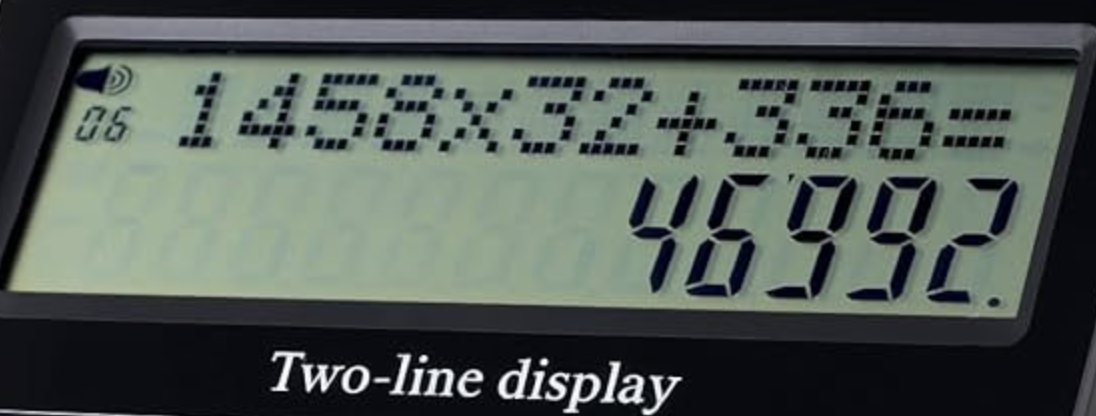
\includegraphics[keepaspectratio]{part_coding/../fig/calculator.png}}

}

\subcaption{\label{fig-basic_cal}Basic calculator}

\end{minipage}%
%
\begin{minipage}[t]{0.50\linewidth}

\centering{

\pandocbounded{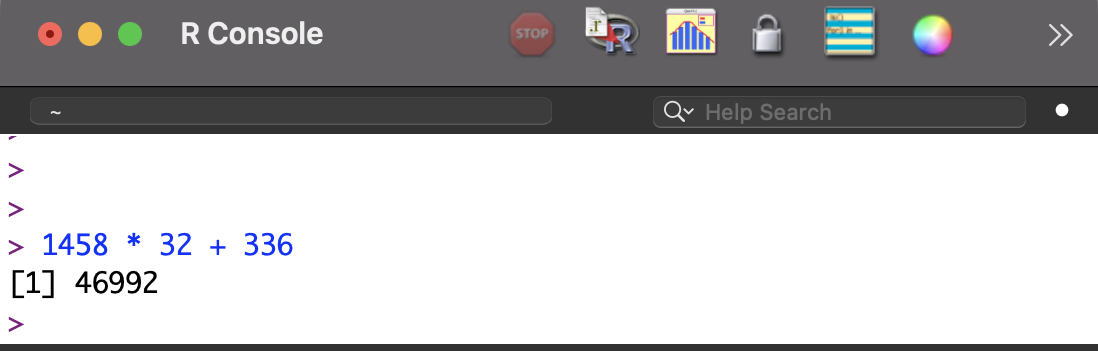
\includegraphics[keepaspectratio]{part_coding/../fig/console_calculation.png}}

}

\subcaption{\label{fig-console}Basic console}

\end{minipage}%

\caption{\label{fig-calculator}Same concept, different interface.}

\end{figure}%

A console functions exactly like the interface of a calculator
Figure~\ref{fig-console}:

\begin{enumerate}
\def\labelenumi{\arabic{enumi}.}
\tightlist
\item
  Type your operation after the ``\textgreater{}'' symbol.
\item
  Press enter/return to evaluate
\item
  The result is displayed under the prompt.
\end{enumerate}

Notice that result is displaed a bit differently (color, not after
\textgreater). And also a new \textgreater{} apperas indivading that it
is waiting for a new

In a conceptual way, the console is the interface that displays your
communication with the program. Shows your input and displays the
output. This simple interface is common to almost all programs.

\section*{Formal}\label{formal-25}
\addcontentsline{toc}{section}{Formal}

\markright{Formal}

ChatGPT: ``The R Console is the interactive text interface where you
communicate directly with the R programming language. It is the place
where you type R commands, press Enter, and immediately see the results
of your code.''

For a program to run, there are four components: the terminal, console,
shell, and kernel

\href{https://www.geeksforgeeks.org/operating-systems/what-is-terminal-console-shell-and-kernel/}{geeklink}

An R Console is an interactive command-line interface (CLI) that allows
users to type R commands directly, execute them immediately, and see
instant output or error messages. It operates on a REPL loop
(Read-Eval-Print Loop):

Read: Accepts user code typed at the prompt. Eval: Evaluates/computes
the code through the R engine. Print: Displays the resulting data, plot
reference, or text. Loop: Displays the prompt again, waiting for the
next command.

\section*{Examples}\label{examples-24}
\addcontentsline{toc}{section}{Examples}

\markright{Examples}

See below interface of three consoles using base R, in RStudio, and in
VS Code.

\begin{figure}

\begin{minipage}[t]{\linewidth}

\centering{

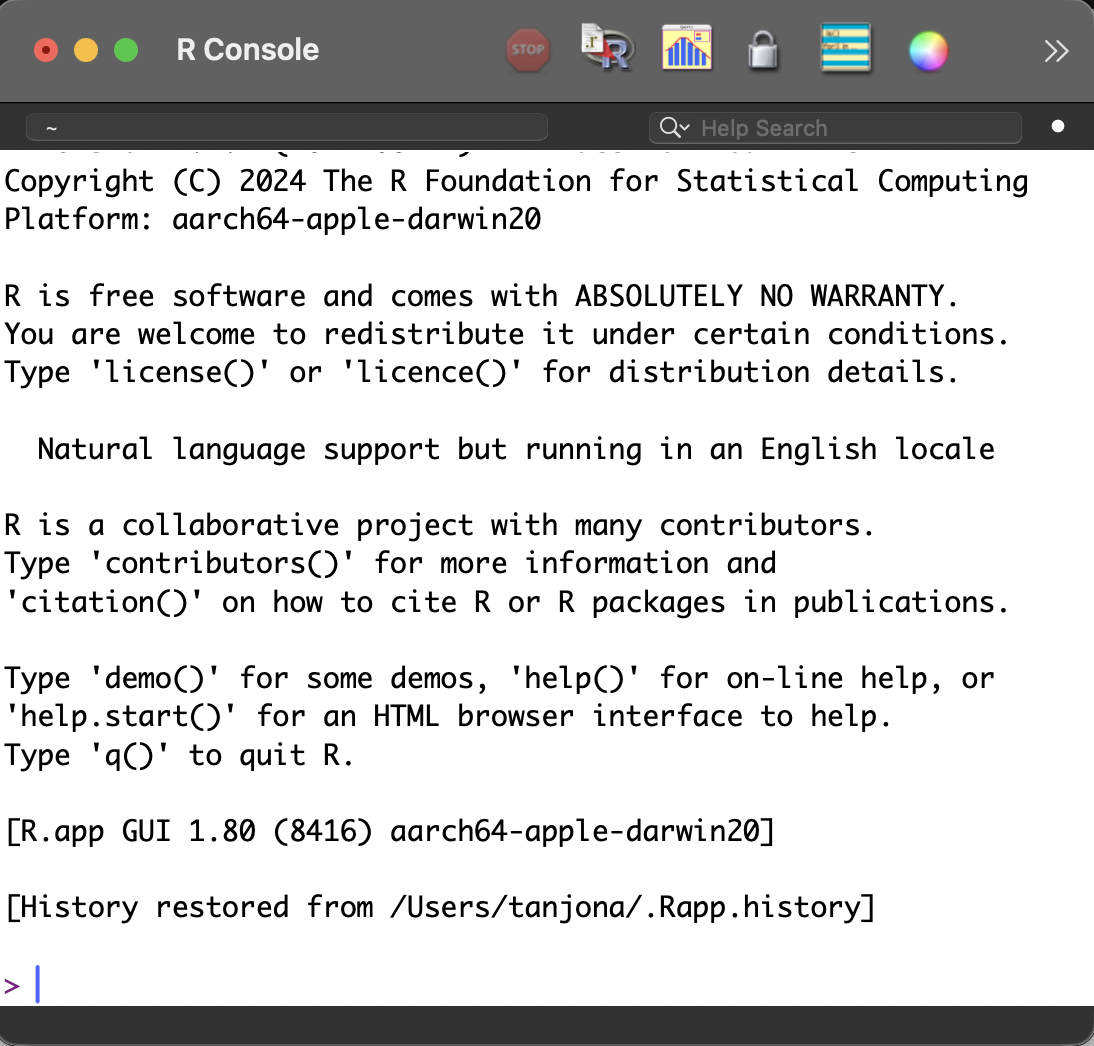
\includegraphics[width=3.125in,height=\textheight,keepaspectratio]{part_coding/../fig/console_r.png}

}

\subcaption{\label{fig-console_default}Console in R}

\end{minipage}%
\newline
\begin{minipage}[t]{\linewidth}

\centering{

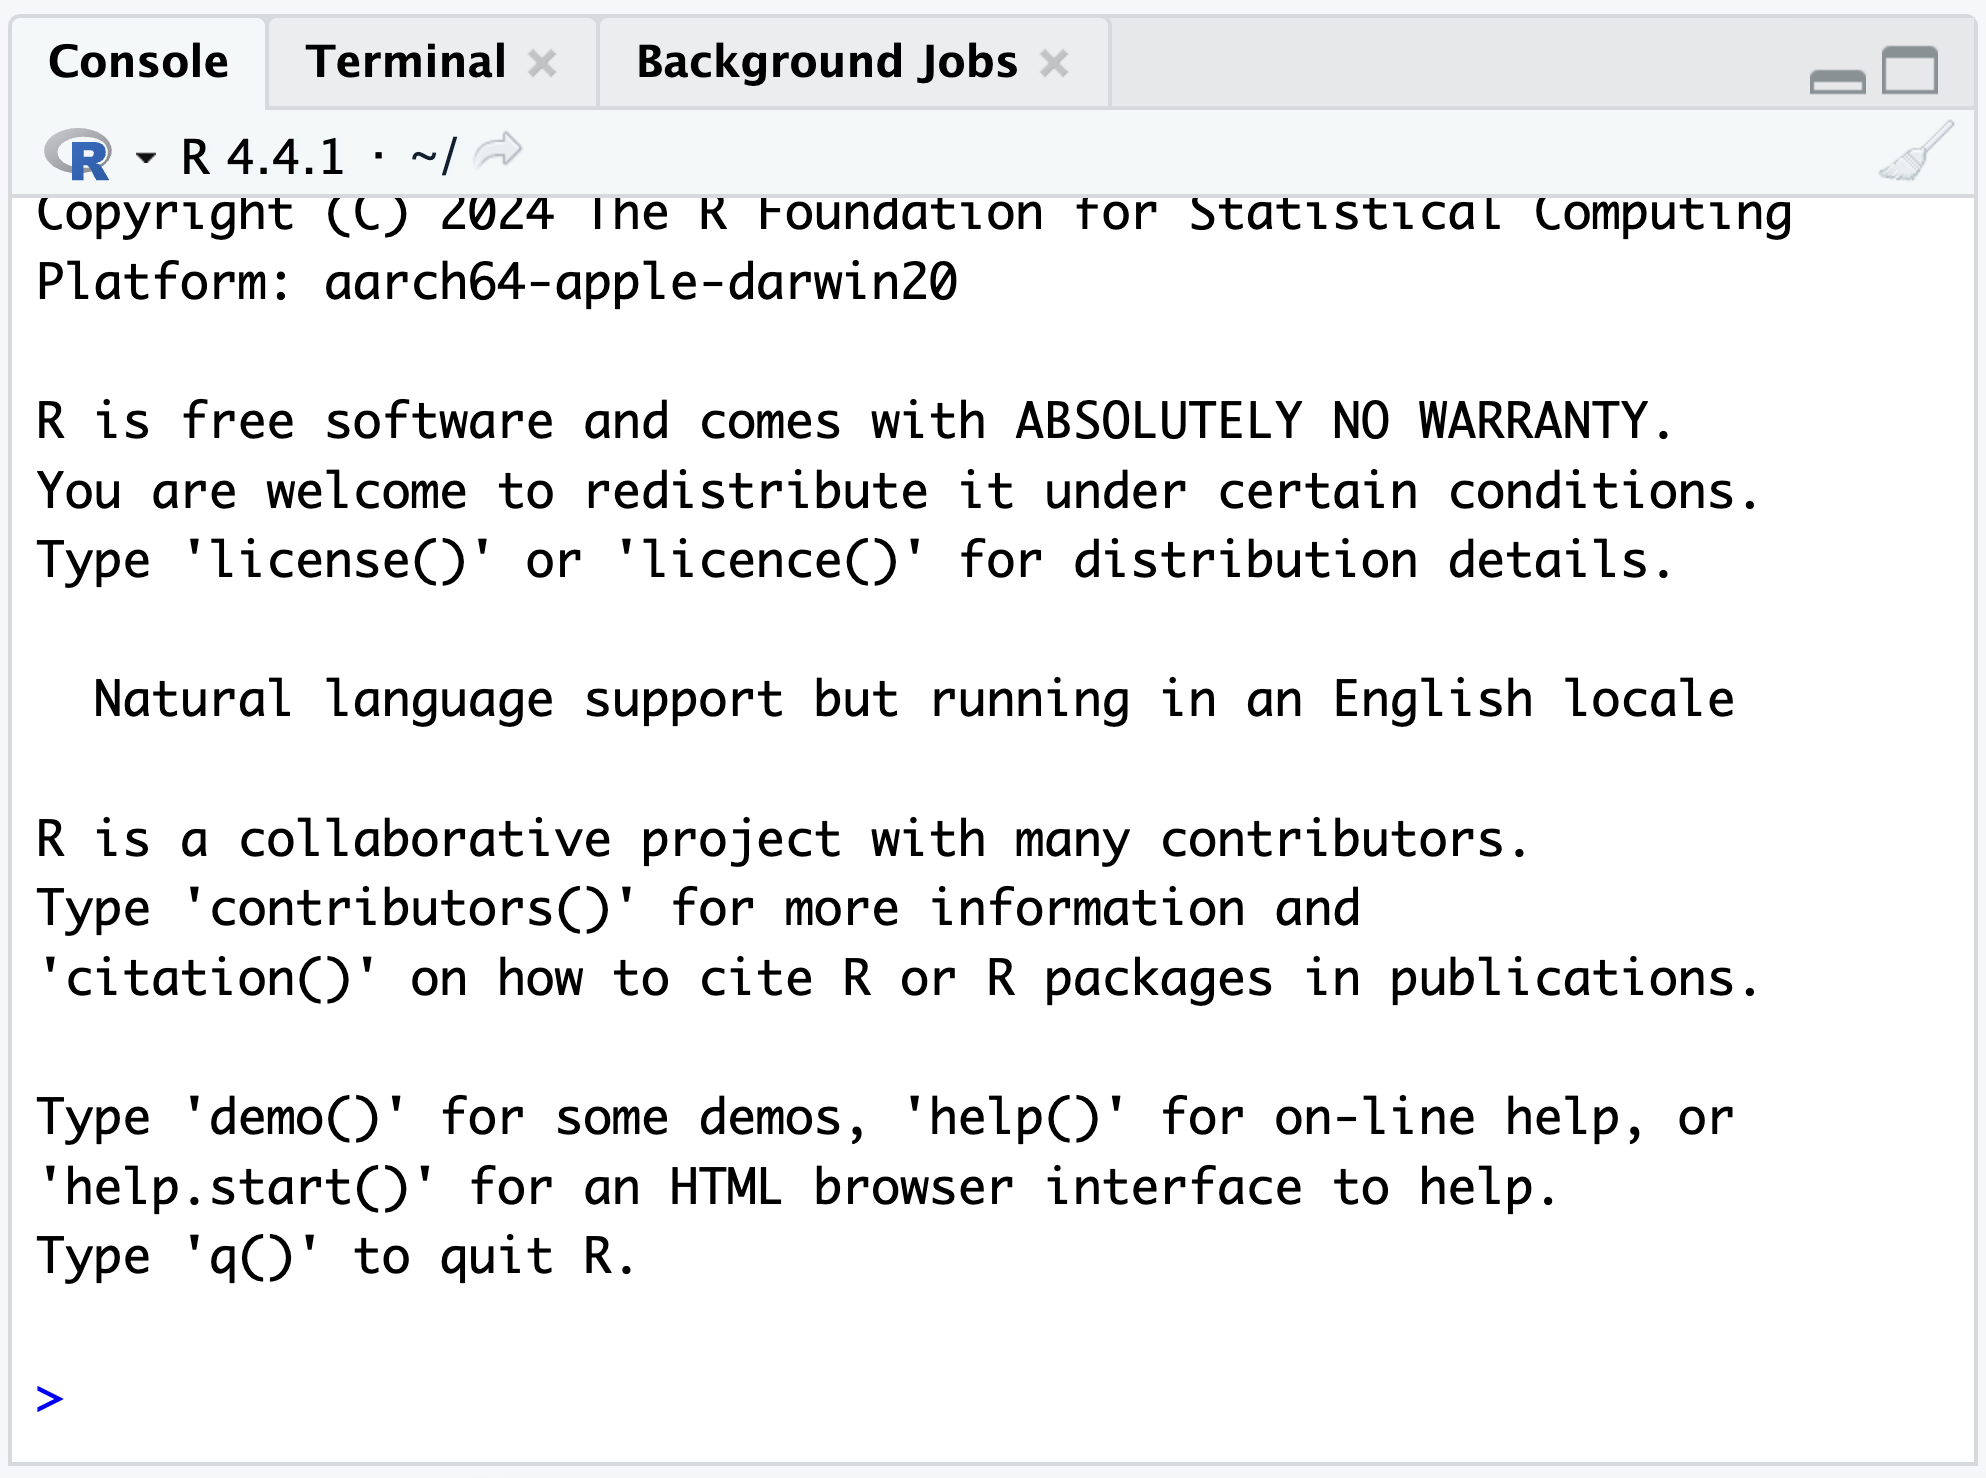
\includegraphics[width=3.125in,height=\textheight,keepaspectratio]{part_coding/../fig/console_rstudio.png}

}

\subcaption{\label{fig-console_rstudio}Console in RStudio}

\end{minipage}%
\newline
\begin{minipage}[t]{\linewidth}

\centering{

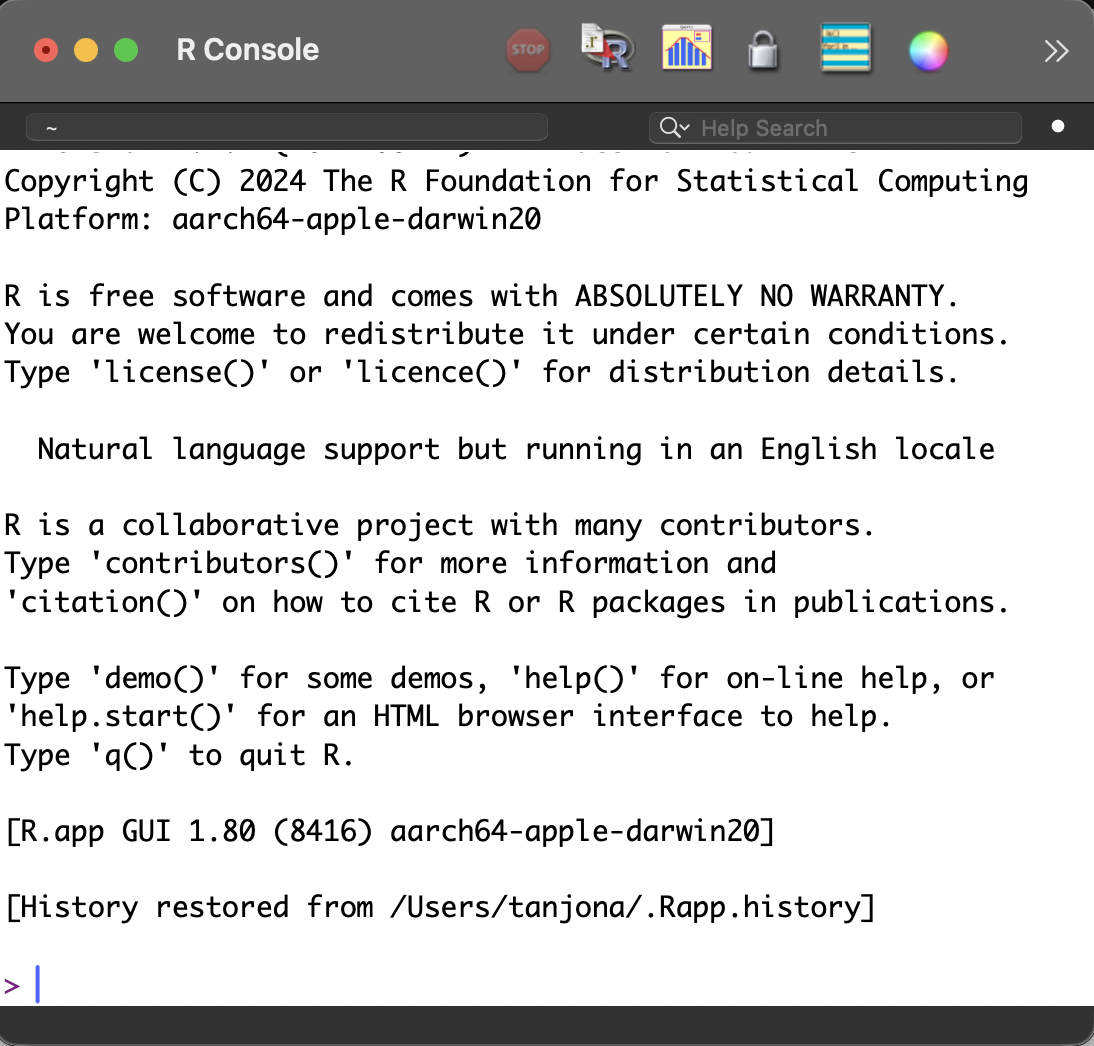
\includegraphics[width=3.125in,height=\textheight,keepaspectratio]{part_coding/../fig/console_vscode.png}

}

\subcaption{\label{fig-console_vscode}Console in VS Code}

\end{minipage}%

\caption{\label{fig-Rconsole}Same concept}

\end{figure}%

As an exercice, you can open R or RStudio and try to input the command
below, the code is in gray and you should see the output as black after
you execute. While you can use copy/paste to do this. It is highly
recommended that you enter the text manually. C

\begin{Shaded}
\begin{Highlighting}[]
\DecValTok{1} \SpecialCharTok{+} \DecValTok{1} \SpecialCharTok{*} \FloatTok{4.1}
\end{Highlighting}
\end{Shaded}

\begin{verbatim}
[1] 5.1
\end{verbatim}

\begin{Shaded}
\begin{Highlighting}[]
\FunctionTok{sin}\NormalTok{(}\DecValTok{123}\NormalTok{)}
\end{Highlighting}
\end{Shaded}

\begin{verbatim}
[1] -0.4599035
\end{verbatim}

\begin{Shaded}
\begin{Highlighting}[]
\FunctionTok{cat}\NormalTok{(}\StringTok{"Hello world"}\NormalTok{)}
\end{Highlighting}
\end{Shaded}

\begin{verbatim}
Hello world
\end{verbatim}

\begin{Shaded}
\begin{Highlighting}[]
\FunctionTok{print}\NormalTok{(}\StringTok{"Hello world"}\NormalTok{)}
\end{Highlighting}
\end{Shaded}

\begin{verbatim}
[1] "Hello world"
\end{verbatim}

\section*{Tips and warnings}\label{tips-and-warnings-18}
\addcontentsline{toc}{section}{Tips and warnings}

\markright{Tips and warnings}

\begin{itemize}
\tightlist
\item
  The kernel is under the hood
\item
  Semantic: Commandline interface, terminal, console moslty mean the
  same thing.
\item
  Unlike a calculator, you don't write your prompt in the (see next
  Chapter~\ref{sec-ide})
\item
  You cannot modify evaluated prompt.
\item
  Your prompt can be incomplete, the program cannot get the answer and
  is asking you to add more input to run the (+) as well as a blinking
  black cursor.
\end{itemize}

\begin{figure}

\centering{

\pandocbounded{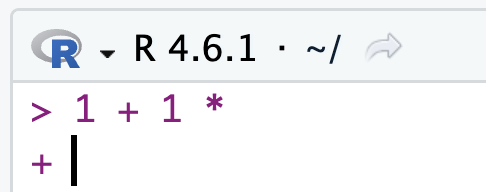
\includegraphics[keepaspectratio]{part_coding/../fig/incomplete_command.png}}

}

\caption{\label{fig-incomplete}Incomplete command}

\end{figure}%

\begin{itemize}
\tightlist
\item
  In that case, you can

  \begin{itemize}
  \tightlist
  \item
    complete the like adding say the number you want to multiply
  \item
    escape the expectation by typing escape key (Echap or Esc)
  \end{itemize}
\item
  \textbf{Error message}: this is the worst part. While we, reading the
  error is very informative and allow to diagnose it.
\item
  Mouse is useless in the console. It is meant to work with keyboard,
\item
  It is not recommended to write prompt on the console\ldots it is
  simple but and a different window called script is dedicated to
  writing code (see Chapter~\ref{sec-ide}).
\item
  When you open the R, or RStudio, you can see the version of the
  program you are using and other licensing information (see
  Figure~\ref{fig-console_rstudio})
\item
  If you close the console/program, all the booking is lost. You can
  save it as what it is called ``Workspace'', but it is not recommended.
\end{itemize}

\chapter{Script editor}\label{sec-script}

Secretaire personel

If you are reading this handbook, it is almost sure that you were, are,
and will use R. In which case, you will have to write, copy, edit,
delete lines and lines of codes. With such a intensive task, it is wise
to make the experience as pleasant, productive, and efficient as
possible.

The essence of a script editor is to assist the coders in all possible
way. The most basic script editor available is just an text editor
(e.g.~Notepad). Yes, it is a script editor because it allows one to
write, edit, and save codes. In fact, in the early days of R, ecologists
wrote code on Notepad, and latter Notepad++. Then copy the chuncks to
execute into the console (Chapter~\ref{sec-console}).

Nowadays, there are many script editors available, but the majority
people are using a stript editor that comes with the IDE
(Chapter~\ref{sec-ide}). To make it more concrete here are few basic
features that enhance code writing:

\textbf{Line numbering}: gives a coordinates to the code. For instance,
one can just say there is an error in line 424. identifies exact lines
when errors occur

\textbf{Identation}: automatically indent the code when hierarchy is
detected.So code structure is easy to scan

\textbf{Syntax highlighting}: different colors for different objects:
number (Chapter~\ref{sec-numeric}), text (Chapter~\ref{sec-character}),
functions (Chapter~\ref{sec-functionCoding}), and comments. So code
structure is easy to scan

\textbf{Bracket \& Parenthesis Matching}: Highlights corresponding
opening and closing brackets (), \{\}, {[}{]} to prevent syntax errors.

There might be different secretary, suits your need to choose the
functionality you need. A programmer codes in many languages like
Python, java, and R might opt for a multi-language script editors. While
the for the average R user, the script editor that comes with RStudio is
the most popular choice.

\section*{Formal}\label{formal-26}
\addcontentsline{toc}{section}{Formal}

\markright{Formal}

A script editor is a specialized text interface used by programmers to
write, edit, and save code files. Unlike an interactive console
(Chapter~\ref{sec-console}) that runs code immediately line-by-line, a
script editor allows you to write out a full sequence of instructions,
review them, and save them as a permanent file before running them.

\section*{Examples}\label{examples-25}
\addcontentsline{toc}{section}{Examples}

\markright{Examples}

\begin{itemize}
\tightlist
\item
  A code look in basic text editor without syntax highlighting and
  indentation
\end{itemize}

\begin{Shaded}
\begin{Highlighting}[]
\NormalTok{\# Add one plus one}
\NormalTok{1 + 1}

\NormalTok{\# Import your data into R}
\NormalTok{data \textless{}{-} read.csv(\textquotesingle{}my\_data.csv\textquotesingle{})}

\NormalTok{\# A ggplot code}
\NormalTok{ggplot(data, aes(x = age, y = height)) +}
\NormalTok{geom\_point()+}
\NormalTok{theme\_bw()}
\end{Highlighting}
\end{Shaded}

\begin{itemize}
\tightlist
\item
  The same code with syntax highlighing different type of object Comment
  in gray, numbers (Chapter~\ref{sec-numeric}) in red, function
  (Chapter~\ref{sec-functionCoding}) is in blue, and character
  (Chapter~\ref{sec-character}) and variable
  (Chapter~\ref{sec-assignment}) in black.
\end{itemize}

\begin{Shaded}
\begin{Highlighting}[]
\CommentTok{\# Add one plus one}
\DecValTok{1} \SpecialCharTok{+} \DecValTok{1}

\CommentTok{\# Import your data into R}
\NormalTok{data }\OtherTok{\textless{}{-}} \FunctionTok{read.csv}\NormalTok{(“my\_data.csv”)}


\CommentTok{\# A ggplot code}
\FunctionTok{ggplot}\NormalTok{(data, }\FunctionTok{aes}\NormalTok{(}\AttributeTok{x =}\NormalTok{ age, }\AttributeTok{y =}\NormalTok{ height)) }\SpecialCharTok{+}
    \FunctionTok{geom\_point}\NormalTok{()}\SpecialCharTok{+}
    \FunctionTok{theme\_bw}\NormalTok{()}
\end{Highlighting}
\end{Shaded}

\begin{itemize}
\tightlist
\item
  A script editor is infused with various features to facilitate coding
  and improve productivity. Here is an example where it will
  suggest/auto-complete the code Figure~\ref{fig-completion}.
\end{itemize}

\begin{figure}

\centering{

\pandocbounded{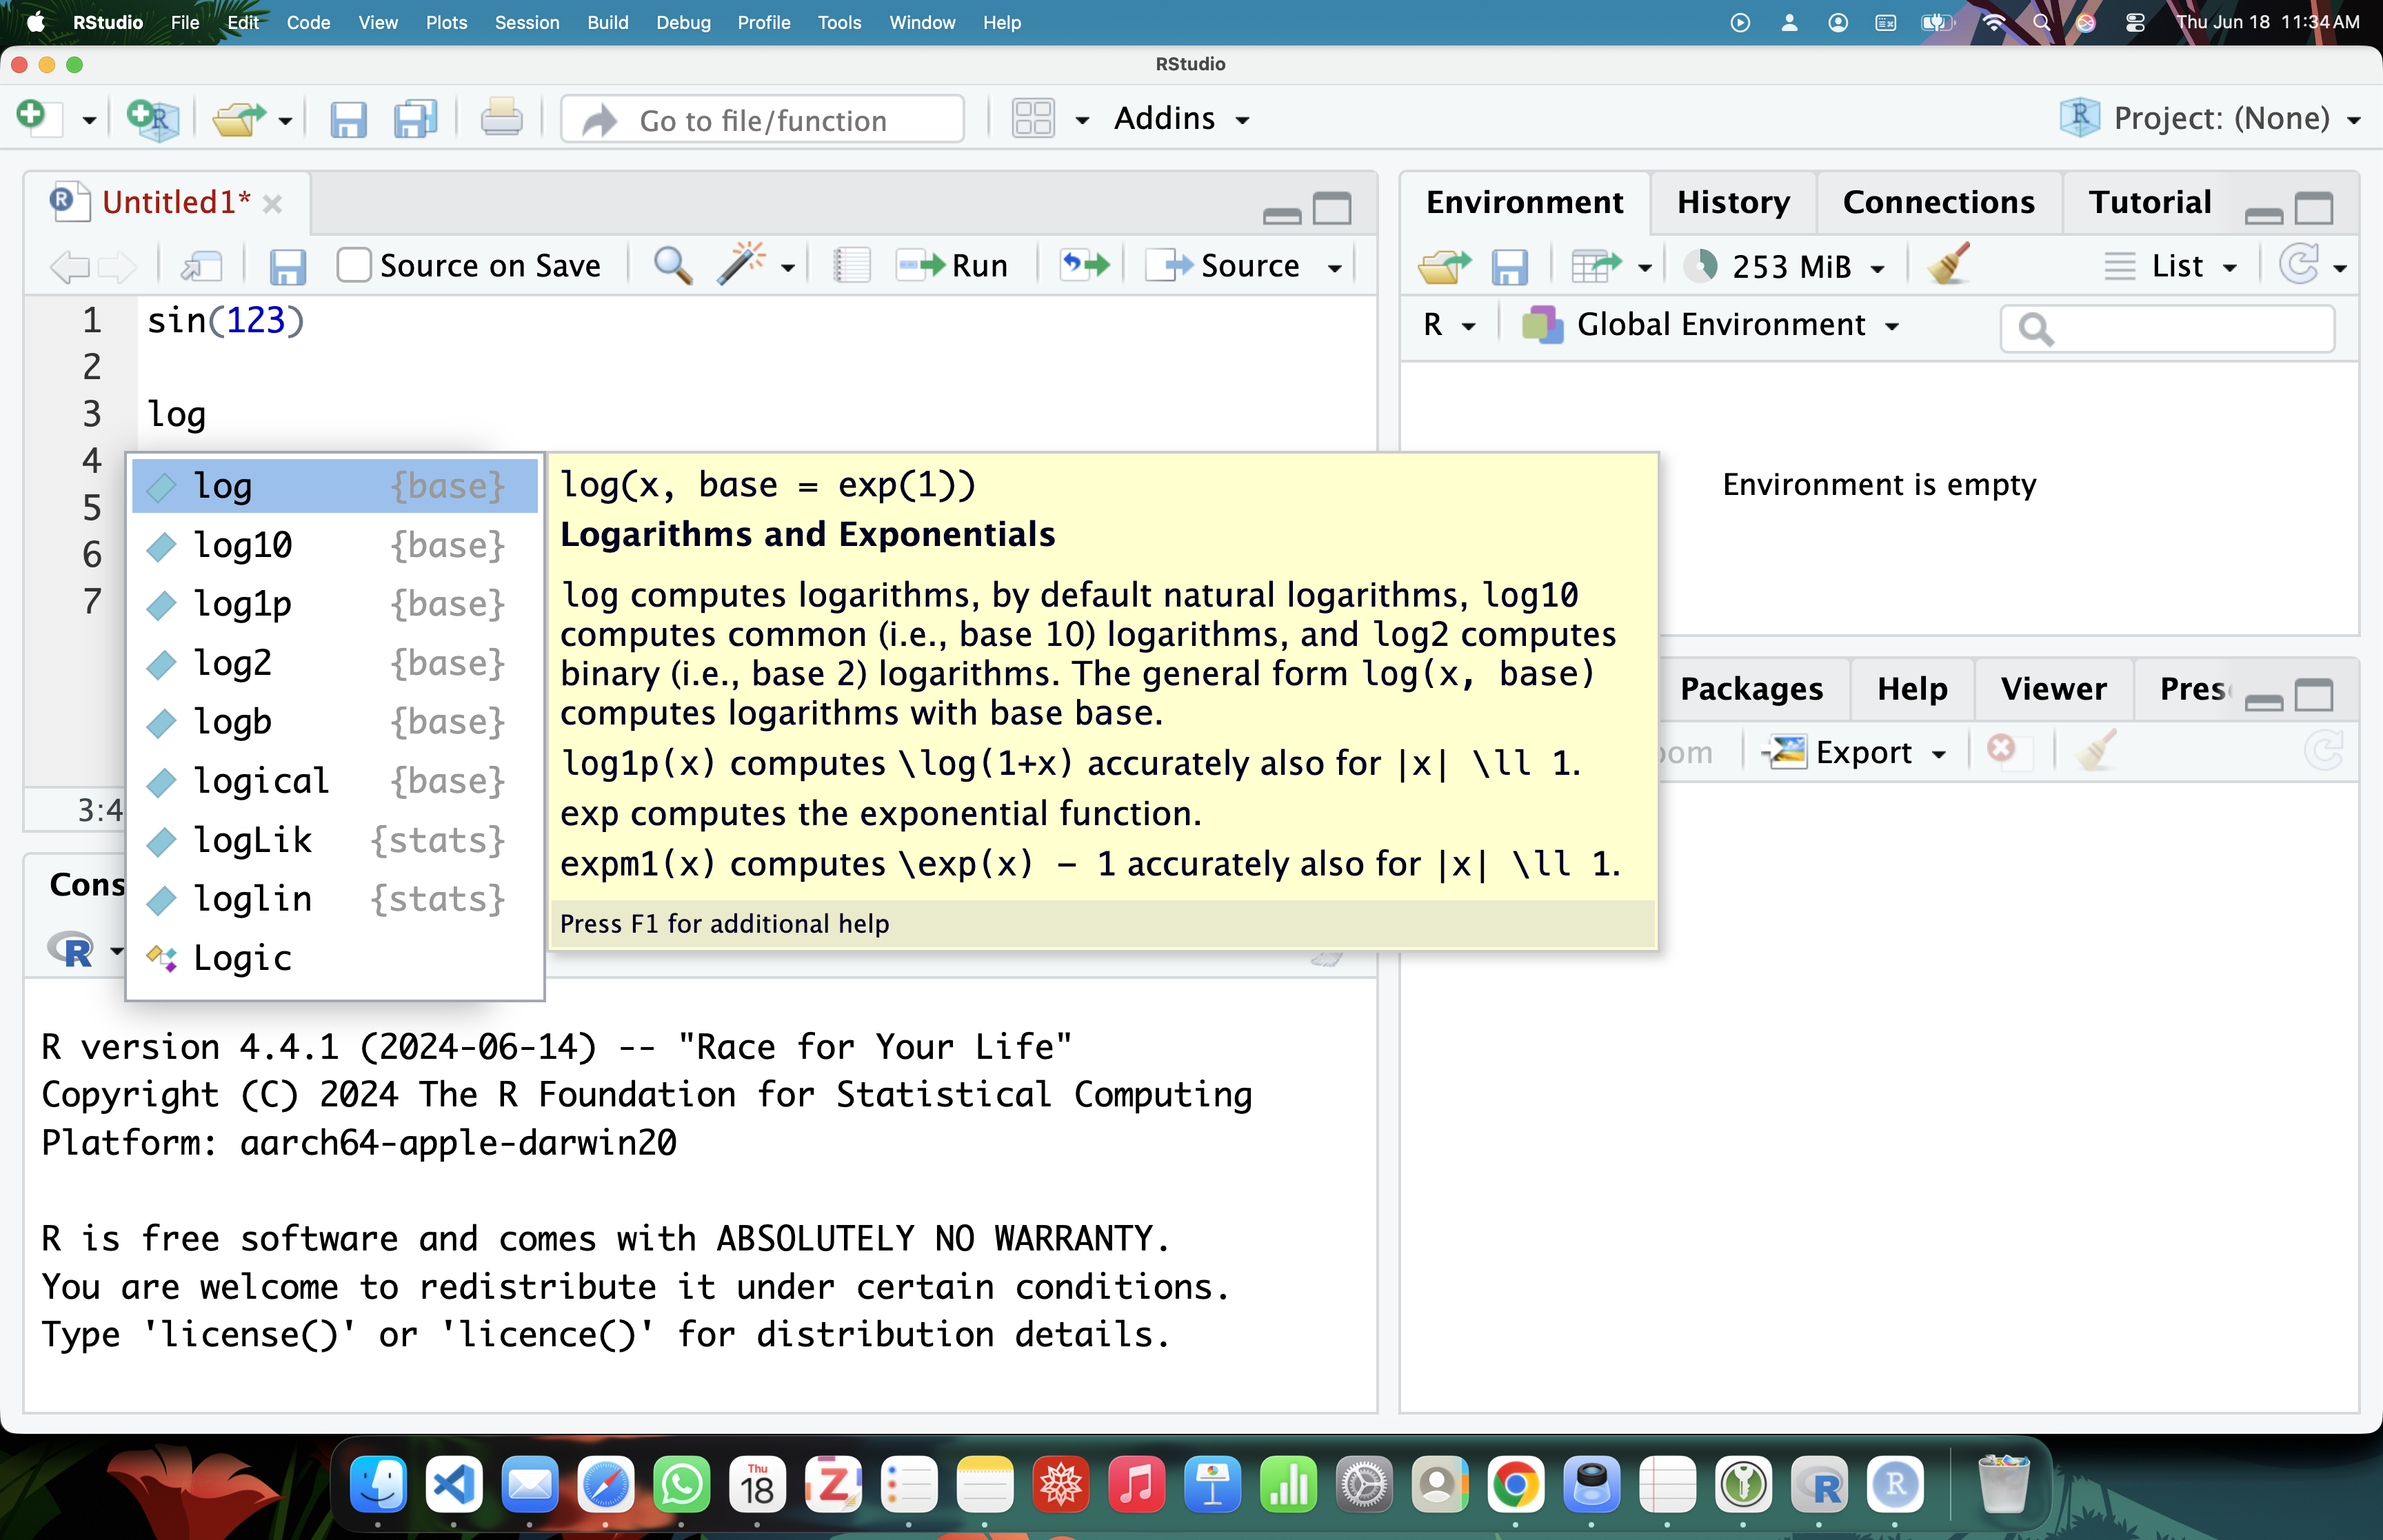
\includegraphics[keepaspectratio]{part_coding/../fig/completion_highlight.png}}

}

\caption{\label{fig-completion}Some features}

\end{figure}%

\section*{Tips and warnings}\label{tips-and-warnings-19}
\addcontentsline{toc}{section}{Tips and warnings}

\markright{Tips and warnings}

\begin{itemize}
\tightlist
\item
  Semantic: code vs script vs program vs commands. It is essentially
  means the collection of instructions that you want the programs to
  evaluate
\item
  \textbf{DO NOT} write codes in console unless it is a one time check.
\item
  Document your code: a good habit yet easy to ignore is to add human.
  While codes are, other people and yourself could benefit from verbale
  description. This is called comment (see gray part preceeded by \#
  above). Practically, it is ignored during the evlation by the
  computer.
\item
  An underused feature of script editors are shortcuts. It is a good
  habit to explore what are available. For instance, shortcut for
  variable assignment \texttt{\textless{}-} this is for instance very
  useful when some symbols are not easily accessible on the keyboard. In
  fact, you can even create your own shortcut. Clicking is slow, typing
  is fast\ldots instead of clikcing the icon, the shortcut is control +
  enter. After few uses you will not notice that like control + S to
  save, control + A to select all.
\item
  Embarce the power: most script editor you will choose are more
  powerful than you think. It could be fun to read and learn some
  features that will make your coding more productive.
\item
  By definition, a script is meant for code writing. To evaluate in the
  console, the brute force is to copy the chunks one wants to run.
  However, there are now features that allows to send the code the
  console while staying the script editor. This is through IDE
  Chapter~\ref{sec-ide}.
\item
  Raw format: codes are written in a raw format. It could opened even in
  word. The syntax are features of the script editor and not the file
  and not the file (unlike word document with bold etc).
\item
  Because it is a raw file is that it could be tracked with a version
  control program.
\item
  Everyone loves to play with the theme. Like a screen shot it is ea but
  can . Themes could be light, dark, colors could be bright, etc.
\end{itemize}

\chapter{IDE: Integrated Development Enviroment}\label{sec-ide}

Secretaire, comptable, avocat personel

The innocent and non-consequential is to confuse R and RStudio. R is a
programming language whereas RStudio is a specialized IDE for R.

As seen a \href{@sec-console}{console}, is the minimum compenent to
code. But as we write code, \href{@sec-script}{script editors} were
created to improve coding (like having a personal secretary to assist in
sometasks). An IDE is the final stage of making coding more comfortable.

To overuse metaphor : R is a car, a script editor is an ensemble of kits
(wheel, leather chair, back camera etc.), and an IDE is a mix of kit
shops, garage, and copilot (in racing not AI).

RStudio is the most popular IDE for R

\section*{Formal}\label{formal-27}
\addcontentsline{toc}{section}{Formal}

\markright{Formal}

An IDE, or Integrated Development Environment, is a a single software
application that provides and combines all the essential tools they need
to write, test, and debug code in one unified interface. Using RStudio
as a main example, an IDE wraps around the basic: - R Console: command
line interface Chapter~\ref{sec-console} - Script editor called Source:
a script editor Chapter~\ref{sec-script} - Environment and history:
(saves history and object created (Chapter~\ref{sec-variable}) and more
- Output: generate figures and more

\begin{figure}

\centering{

\pandocbounded{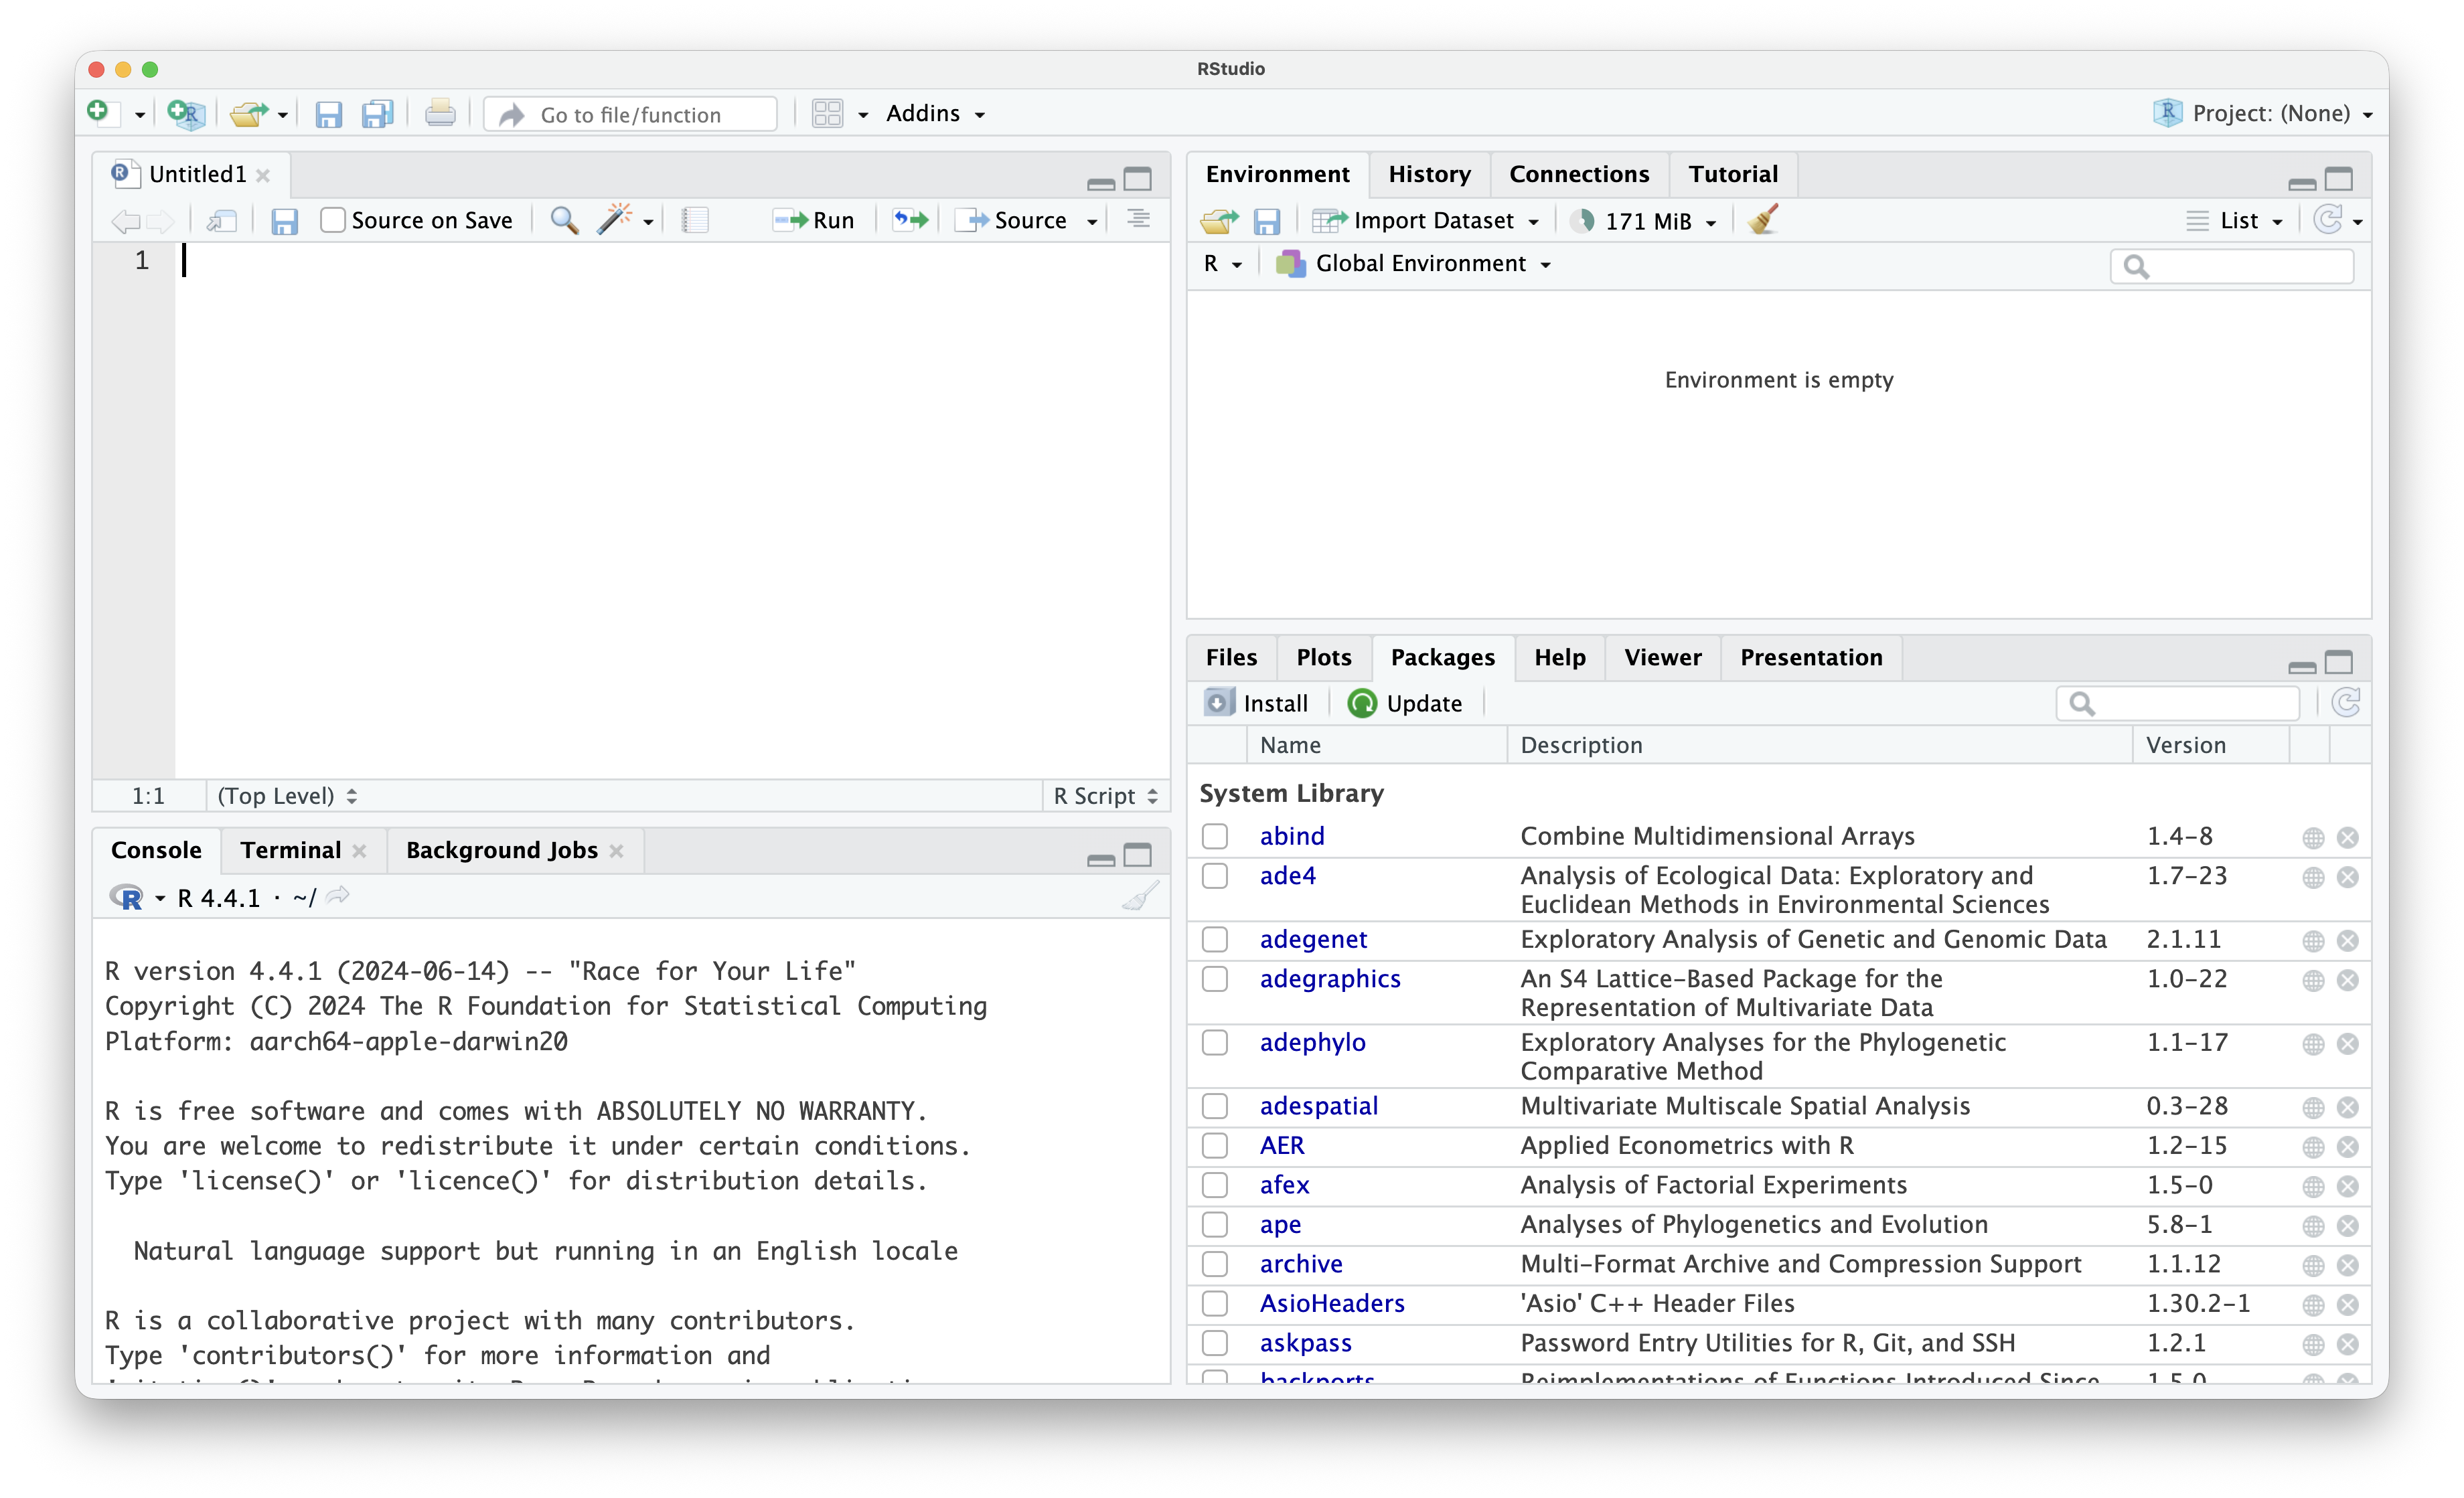
\includegraphics[keepaspectratio]{part_coding/../fig/RStudio.png}}

}

\caption{\label{fig-RStudio}Starting RStudio}

\end{figure}%

Instead of writing code in a basic text editor, executing it in a
separate terminal, and opening another window to view graphs, an IDE
consolidates these workflow components under a single workspace.

\section*{Examples}\label{examples-26}
\addcontentsline{toc}{section}{Examples}

\markright{Examples}

Step 1: One can write all the codes in one file

\begin{figure}

\centering{

\pandocbounded{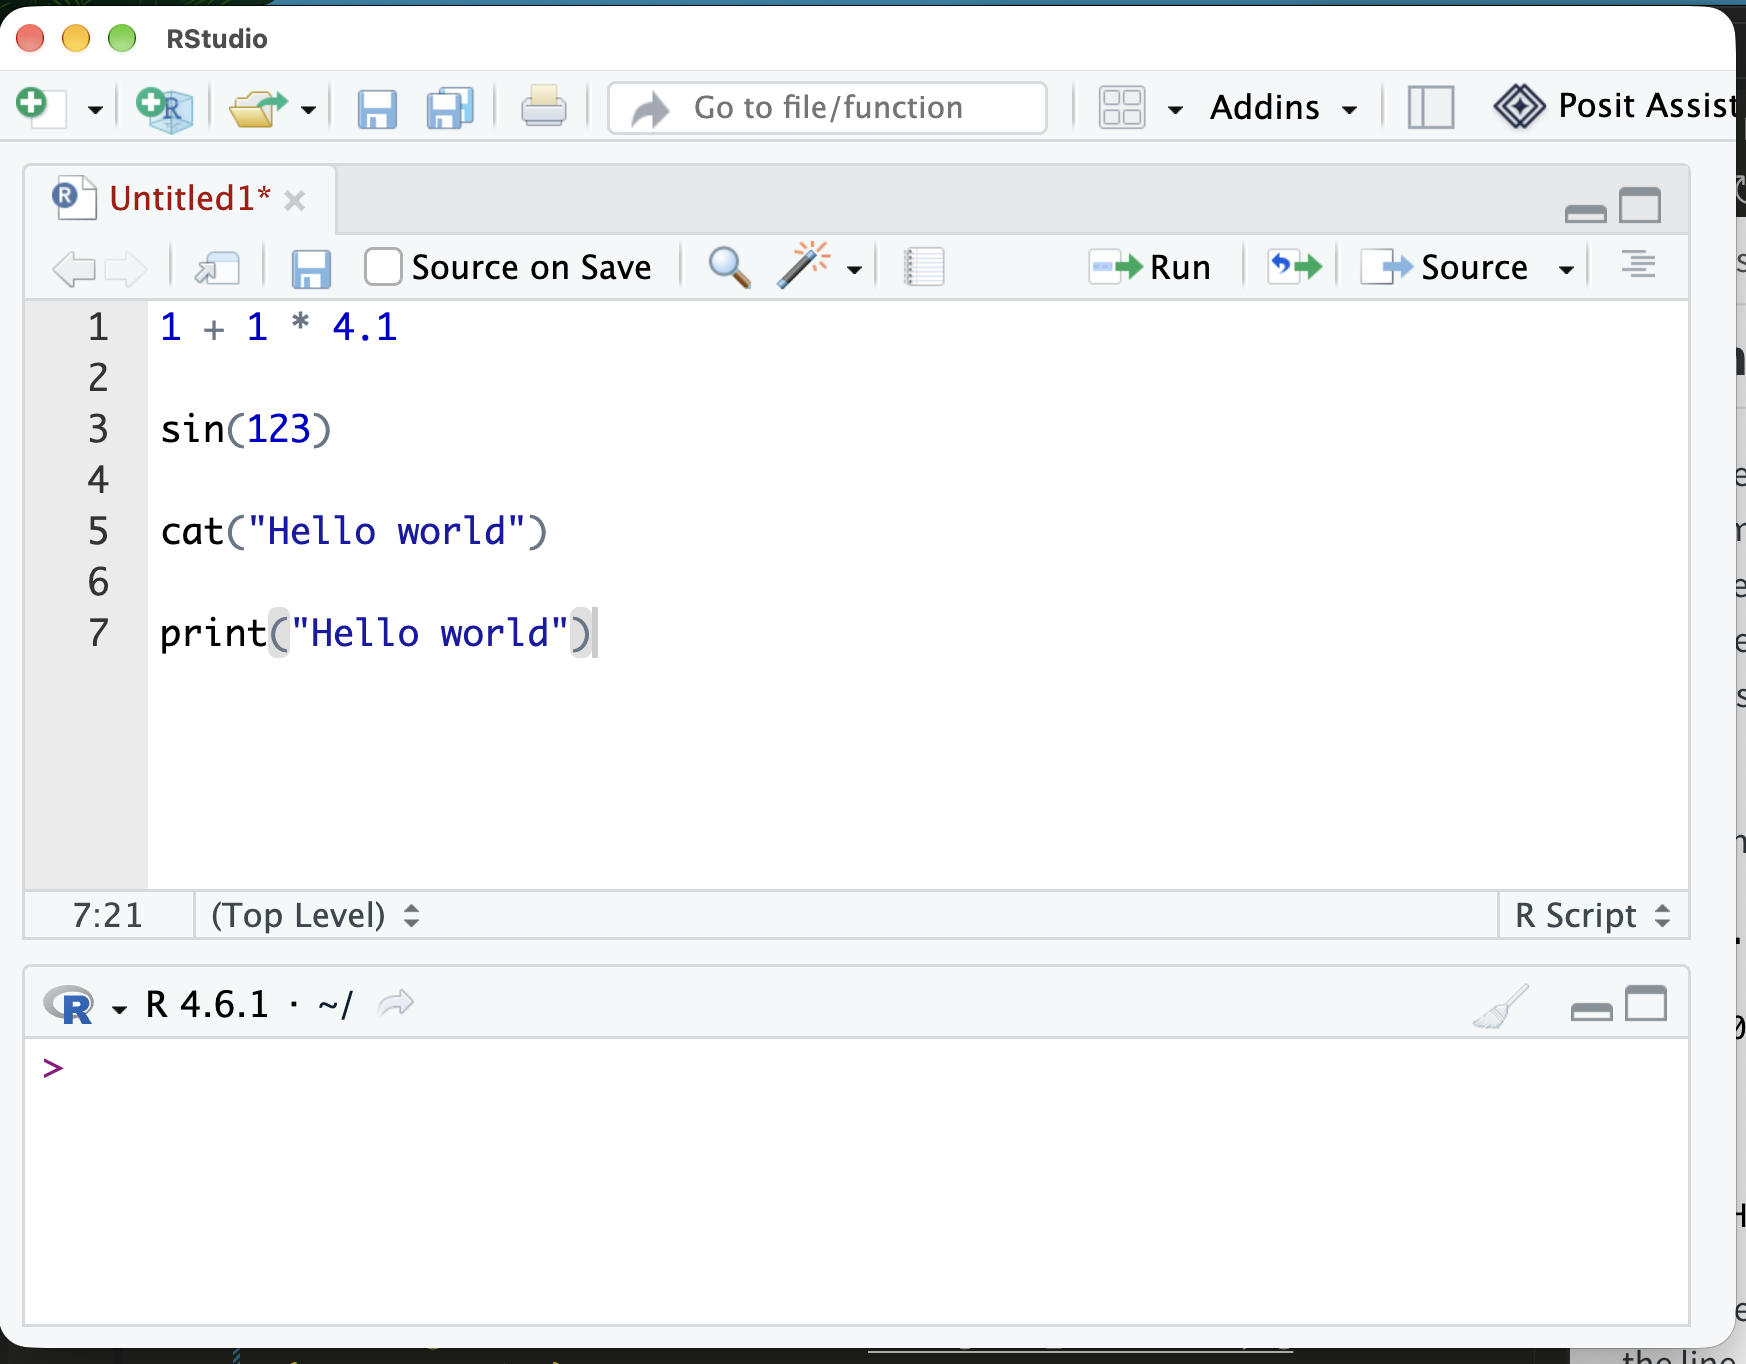
\includegraphics[keepaspectratio]{part_coding/../fig/write_script.png}}

}

\caption{\label{fig-simple_script}Write all the scripts in the previous
section}

\end{figure}%

Step 2: evaluate. Two ways to evaluate: Click on the icon run after
placing the cursor in the line

\begin{itemize}
\item
  line evaluation here place the cursor in line 5 not where in the line.
  \pandocbounded{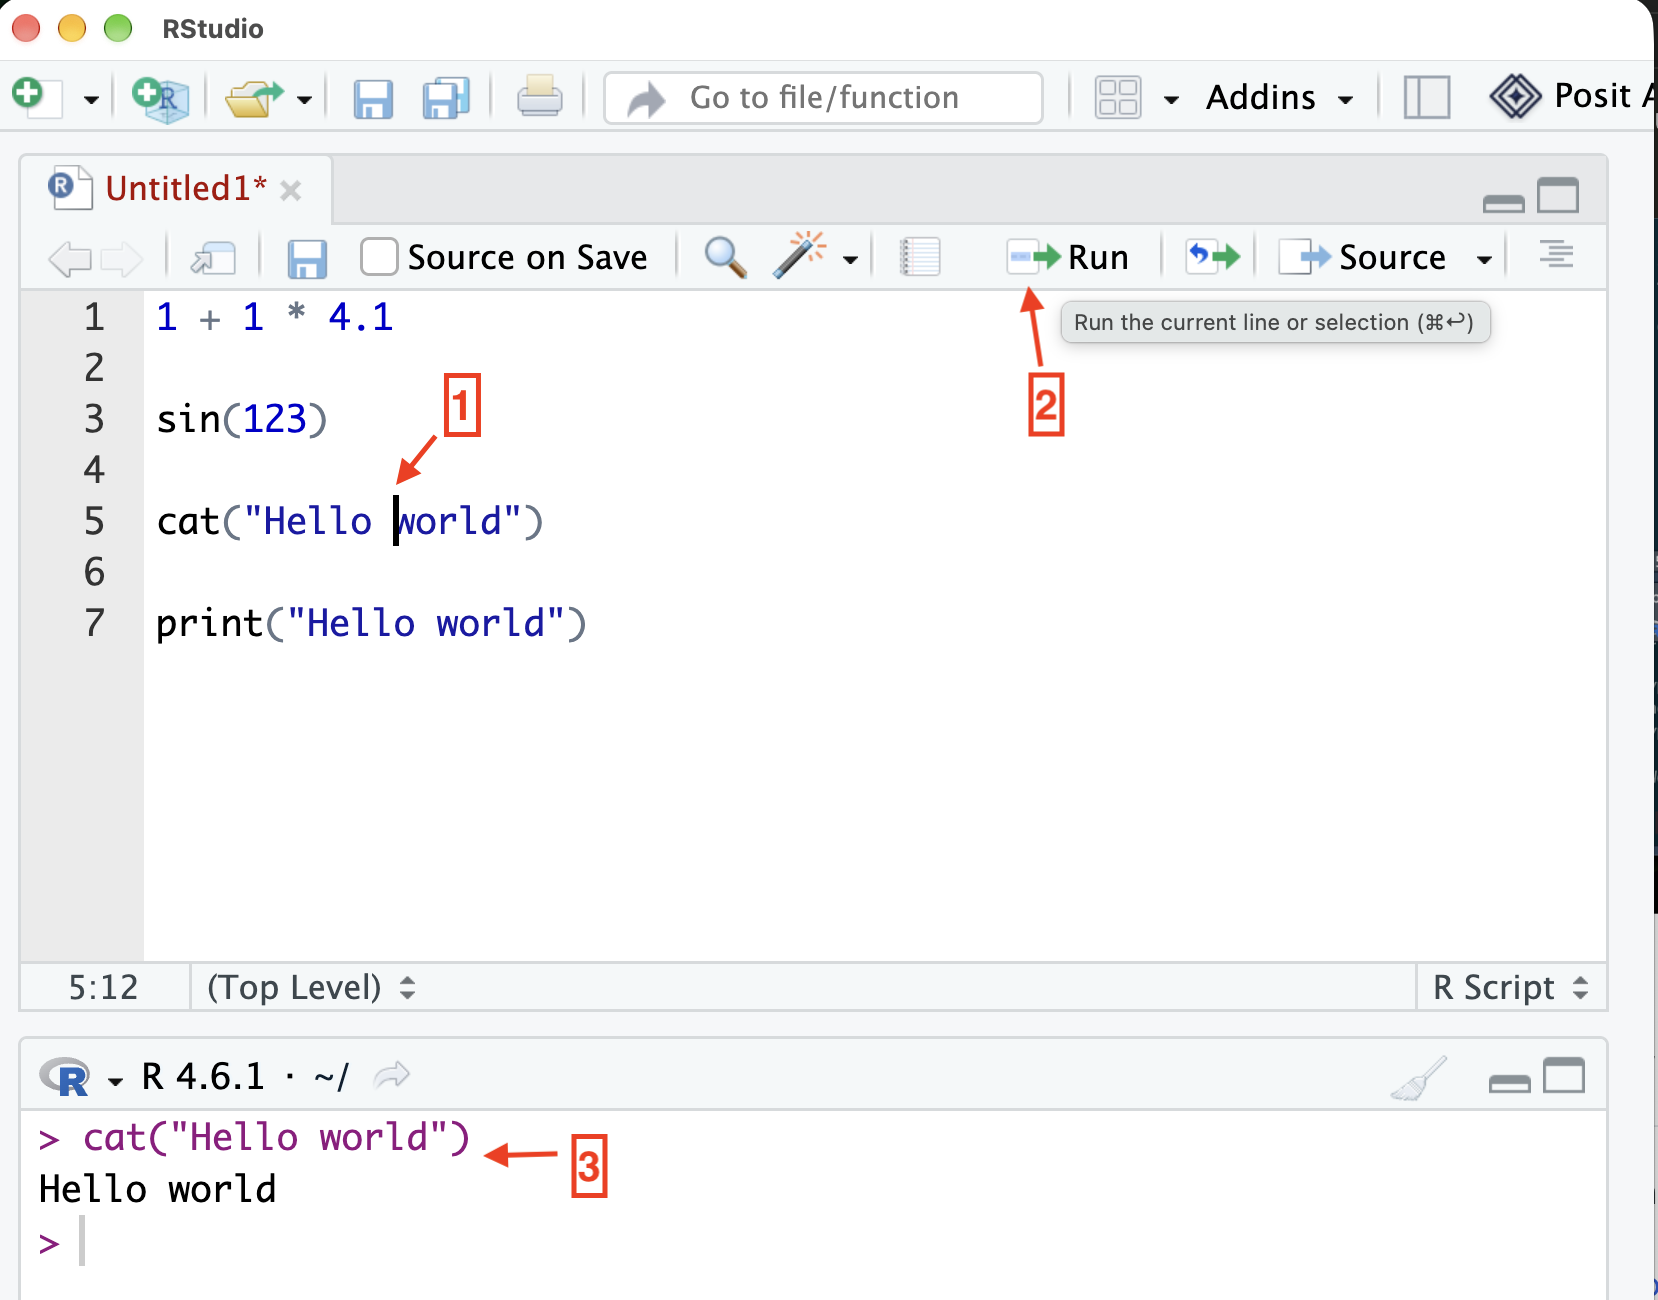
\includegraphics[keepaspectratio,alt={Running the line 5}]{part_coding/../fig/run_one_line.png}}
\item
  selection evaluation: select the code chunk
  \pandocbounded{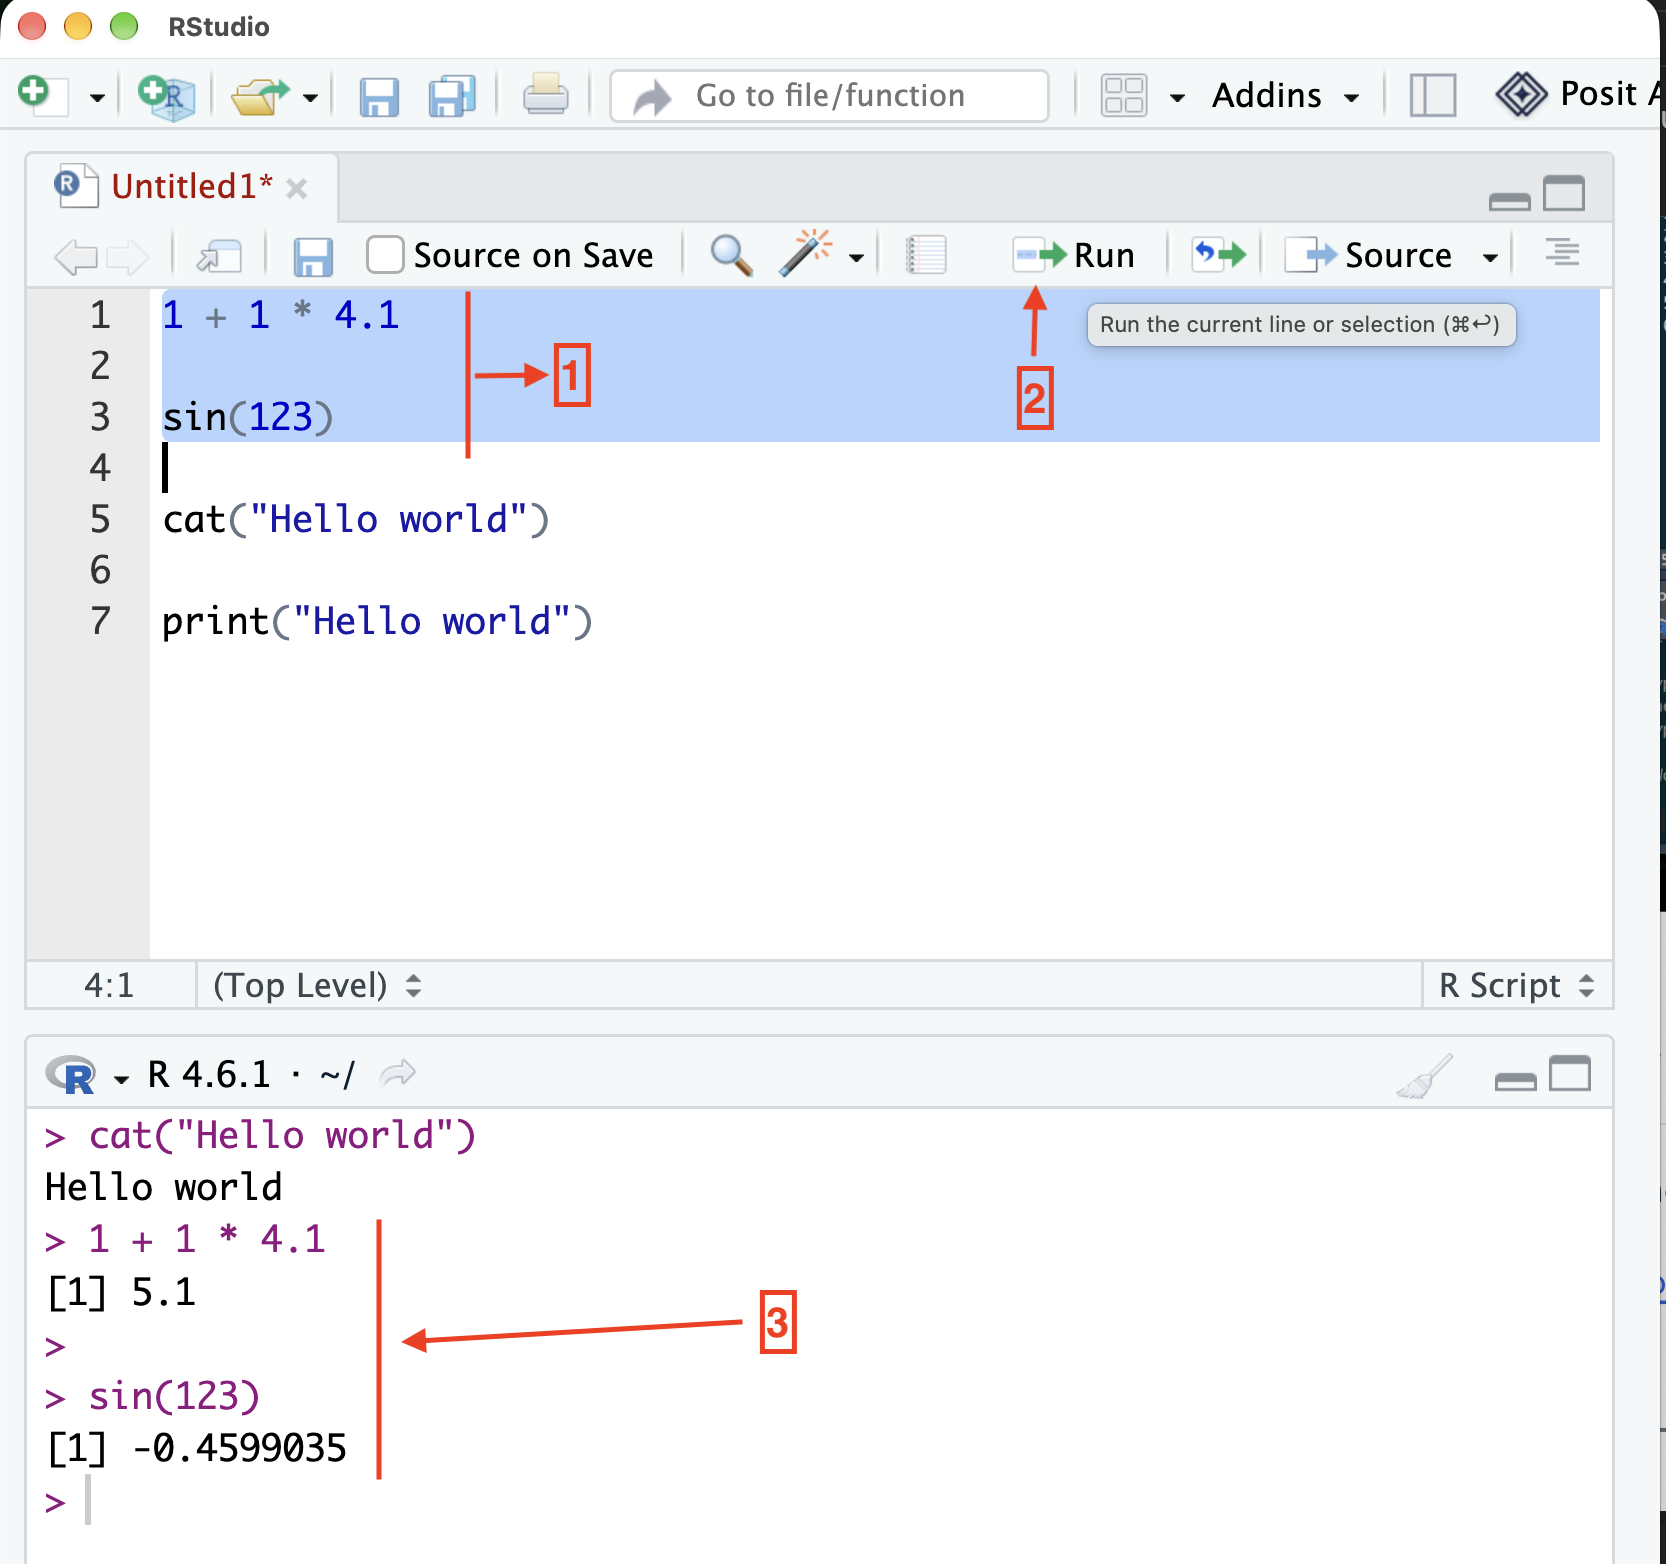
\includegraphics[keepaspectratio,alt={Running code from line 1 to 3}]{part_coding/../fig/run_selection.png}}
\end{itemize}

\section*{Tips and warnings}\label{tips-and-warnings-20}
\addcontentsline{toc}{section}{Tips and warnings}

\markright{Tips and warnings}

\begin{itemize}
\tightlist
\item
  R GUI is getting better. The native and this include script, native
  code running, pacakge manager etc. It could be instructive to compare
  the two. Sometimes, RStudio is have or have issue using native is
  always available
\item
  Underused enviromnent tab/pane: this list all the object created
  during R session. Quite useful for keeping track of all the object
  created and peak at their values.
\item
  Friendly bottom-left pane. While coding consists of writing, that pane
  allows to use more natiral mouse click to navigate folder, import
  file, install and load packages, look for documentation and more
\item
  Version control was also in RStudio
\item
  \href{https://docs.posit.co/ide/user/}{Documentation for RStudio}
\item
  Positron might be next evolution of RStudio, especially if one also
  codes in python
\end{itemize}

\chapter{Object assigment}\label{sec-assignment}

Toko telo

\texttt{sary\_mainitirano.jpeg,\ foza\ orana.mp3,\ Malok\textquotesingle{}ila\_1.mp4}
Beyond clicking these files on your computer, have you wondered how it
works?

Say you change the filename (rename the file), for example:
\texttt{sary\_maintirano.jpeg} to \texttt{sary\_paris.jpeg}. When you
open that, the photo is still the photo you took in Maintirano. In other
words, the filename is something symbolic, a label created by the user
to infer the content. Isn't it frustrating to find a file where you have
now idea what it's inside unless you open it!

In the most fundamental way, a file content is a long sequence of 0 and
1 stored in the computer's memory. To access the sequence, we need the
address (coordinate of that sequence). Figuratively, the filename is
like name of the house (e.g.~Villa Fanomezana), it can change but the
house and the address is the same and generally does not change.

In programming, an assignment consist of binding three elements: (1)
creating an object (building a house) at the specific location (the
address) and calling it whatever you like. While you can choose which
object you create and how to call it is, you cannot decide about the
address (where it is put in the computer.) And probably a good thing.

\section*{Formal}\label{formal-28}
\addcontentsline{toc}{section}{Formal}

\markright{Formal}

In R, the syntax is:
\texttt{filename/variablename\ \textless{}-\ object/value} which reads
put the object in a variable called filename. The assignment operator
essentially creates a new filename, makes a new address and stores the
created object there.

In the study of programming language design, assignment is defined as a
mechanism that dynamically changes the binding between a state storage
location and a value. It introduces the foundational concept of L-values
(location/address) and R-values (read/data value)(wikipedia)

Object can be almost anything, in fact the rest of this part is about
different types of fundamental objects from Chapter~\ref{sec-numeric} to
Chapter~\ref{sec-list}.

The notion of variable has now appeared in three field: in mathematics,
in statistics Chapter~\ref{sec-variable}, and also in R. In fact the
variable name is also called a variable. Obviously, it does not mean the
same thing. This is inevitable in three flourishing field that have some
similarities. Yet, it is a good exercise to see the nuances.

\section*{Examples}\label{examples-27}
\addcontentsline{toc}{section}{Examples}

\markright{Examples}

In the first example, one stores the number \texttt{2} in an object
called \texttt{a}. If you run the that line in R, there will be no
output in the console. You asked R to save the file, not to play it. To
see the content you need to type the filename

\textbf{Assignment and console output}

\begin{Shaded}
\begin{Highlighting}[]
\NormalTok{a }\OtherTok{\textless{}{-}} \DecValTok{2}
\CommentTok{\# no output}

\CommentTok{\# this will display the ouptut in a}
\NormalTok{a}
\end{Highlighting}
\end{Shaded}

\begin{verbatim}
[1] 2
\end{verbatim}

** Adding numbers by their name **

Instead of adding \texttt{2\ +\ 3} we can put 2 in a and 3 in b. And add
\texttt{a\ +\ b} and put them in c. Notice again that the variable names
are symbolic.

\begin{Shaded}
\begin{Highlighting}[]
\CommentTok{\# Storing a number}
\NormalTok{a }\OtherTok{\textless{}{-}} \DecValTok{2}

\NormalTok{b }\OtherTok{\textless{}{-}} \DecValTok{3}

\CommentTok{\# Storing the result a calculation}

\NormalTok{c }\OtherTok{\textless{}{-}}\NormalTok{ a }\SpecialCharTok{+}\NormalTok{ b}
\end{Highlighting}
\end{Shaded}

\textbf{Swapping value} A very educative exercice to understand
assigment is by swapping the content inside two objects.

\begin{Shaded}
\begin{Highlighting}[]
\CommentTok{\# Swapping elements between box}
\NormalTok{object1 }\OtherTok{\textless{}{-}} \DecValTok{1}
\NormalTok{object2 }\OtherTok{\textless{}{-}} \DecValTok{2}

\NormalTok{object2 }\OtherTok{\textless{}{-}}\NormalTok{ object1}
\NormalTok{object1 }\OtherTok{\textless{}{-}}\NormalTok{ object2}

\NormalTok{object1 }\CommentTok{\# to see what is inside object1}
\end{Highlighting}
\end{Shaded}

\begin{verbatim}
[1] 1
\end{verbatim}

\begin{Shaded}
\begin{Highlighting}[]
\NormalTok{object2 }\CommentTok{\# to see what is inside object2}
\end{Highlighting}
\end{Shaded}

\begin{verbatim}
[1] 1
\end{verbatim}

It does not work, the value inside object1 becomes 1 (no swap), and
object2 becomes 1.

The solution is to think you put juice in a cup and coffee in a glass.
To swap the content, you first need transfer one of the beverage in a
thrid container, the proceed.

\begin{Shaded}
\begin{Highlighting}[]
\NormalTok{temporary }\OtherTok{\textless{}{-}}\NormalTok{ object1}
\NormalTok{object1 }\OtherTok{\textless{}{-}}\NormalTok{ object2}
\NormalTok{object2 }\OtherTok{\textless{}{-}}\NormalTok{ temporary}
\end{Highlighting}
\end{Shaded}

\section*{Tips and warnings}\label{tips-and-warnings-21}
\addcontentsline{toc}{section}{Tips and warnings}

\markright{Tips and warnings}

\begin{itemize}
\tightlist
\item
  Semantic: variable name, symbol, scope?
\item
  Object name is case sensitive, \texttt{my\_object\ \textless{}-\ 2},
  \texttt{my\_Object\ \textless{}-\ 2}, and
  \texttt{my\_obJect\ \textless{}-\ 2} are three different objects
  different address and different variable names.
\item
  The most common error in programing seen below
  Figure~\ref{fig-objectError} . While it is a source of panic, it is
  the easiest to solve and the main culprit are

  \begin{itemize}
  \tightlist
  \item
    typos because it is case sensitive
  \item
    variable not assigned. One has typed the script but did not execute
    so it is not stored in the environment
  \end{itemize}
\end{itemize}

\begin{figure}

\centering{

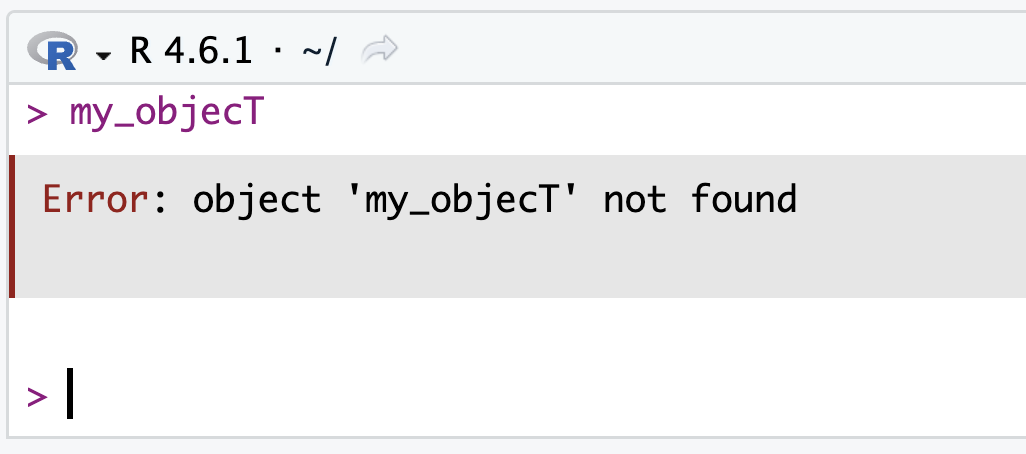
\includegraphics[width=0.6\linewidth,height=\textheight,keepaspectratio]{part_coding/../fig/object_not_found.png}

}

\caption{\label{fig-objectError}Object not found}

\end{figure}%

\begin{itemize}
\tightlist
\item
  In R, one can also use = as an object assignment, \texttt{a\ =\ 2}
  works too. However, the \textless- is to be explicit. So that = is
  used in a specific context
\item
  In later version of R, the symbol -\textgreater{} (left to right) has
  been added \texttt{2\ -\textgreater{}\ a}.
\item
  In the code below, you can the crush the previous value and will be
  lost. See swapping above
\item
  It is a good idea and a good habit to make a variable evocative so you
  can get the content ()
\item
  Variable names convetion

  \begin{itemize}
  \tightlist
  \item
    \textbf{No space} and special characters (\%, \$ etc.)
  \item
    Cannot start with a number or uncerscore
  \item
    Multiwords:

    \begin{itemize}
    \tightlist
    \item
      TelmaNumber and MadacomNumber (called PascalCase)
    \item
      Telma-Number and Madacom-Number (called Kebab Case)
    \item
      telmaNumber and madacomNumber (called camelCase)
    \item
      telma\_number and madacom\_number (called snake\_case)
    \item
      TELMA\_NUMBER and MADACOM\_NUMBER (called screaming snake\_case)
    \item
      telma.number and madacom.number (informal dot.case no longer used)
    \end{itemize}
  \end{itemize}
\item
  A short cut for \textless- is in RStudio on Windows.
\item
  The top right panel will show all the object created with the name and
  the value
\end{itemize}

\chapter{Type: Integer and numeric}\label{sec-numeric}

The machine version of discrete and continuous number

Programs are to calculate, the natural object that you can create,
store, and manipulate are numbers. There are two types of numbers
following the concepts in mathematics
Chapter~\ref{sec-discrete_continuous} and in statistics
Chapter~\ref{sec-quantitative-variable}.

Discrete variables (or whole number) are represented by
integer--truenoymy (vs mysnomy) used for counting and indexing.

In R programming, a real number (continuous) is called numeric.

While it is important to know these distinctions, in general R is very
relaxed about the two types, and say smart enough that it would complain
if you mistakenly use that is supposed to be an integer. For instance,
you can use numeric to specific the length of a vector, or as indexing.

\section*{Formal}\label{formal-29}
\addcontentsline{toc}{section}{Formal}

\markright{Formal}

To force R to read a number as integer, we add L after the number

\begin{Shaded}
\begin{Highlighting}[]
\NormalTok{my\_favorite\_integer }\OtherTok{\textless{}{-}} \DecValTok{24}\NormalTok{L}
\end{Highlighting}
\end{Shaded}

A numeric is generally a number with decimals. The decimal separator in
programming language (Excel is not a programming language) is a period
``.'' Comma is used as a list separator (see Chapter~\ref{sec-vector},
Chapter~\ref{sec-matrixCoding}, and Chapter~\ref{sec-list}).

\begin{Shaded}
\begin{Highlighting}[]
\NormalTok{a\_real\_number }\OtherTok{\textless{}{-}} \FloatTok{24.022}
\end{Highlighting}
\end{Shaded}

If the L is not specificed, R automatically assume that the value is
numeric

\begin{Shaded}
\begin{Highlighting}[]
\NormalTok{my\_favorite\_integer }\OtherTok{\textless{}{-}} \DecValTok{24}
\end{Highlighting}
\end{Shaded}

\section*{Examples}\label{examples-28}
\addcontentsline{toc}{section}{Examples}

\markright{Examples}

\begin{Shaded}
\begin{Highlighting}[]
\CommentTok{\# some constants are directly implemented/have their own notation}
\NormalTok{pi}
\end{Highlighting}
\end{Shaded}

\begin{verbatim}
[1] 3.141593
\end{verbatim}

\begin{Shaded}
\begin{Highlighting}[]
\CommentTok{\# the square root of two is a numeric}
\FunctionTok{sqrt}\NormalTok{(}\DecValTok{2}\NormalTok{)}
\end{Highlighting}
\end{Shaded}

\begin{verbatim}
[1] 1.414214
\end{verbatim}

\begin{Shaded}
\begin{Highlighting}[]
\CommentTok{\# assign a number}
\NormalTok{my\_number }\OtherTok{\textless{}{-}} \FloatTok{2.13}

\NormalTok{a }\OtherTok{\textless{}{-}} \DecValTok{2}\NormalTok{L}
\NormalTok{cc }\OtherTok{\textless{}{-}} \DecValTok{2}

\CommentTok{\# The function str here assess the type of the object. Here it is an integer}
\FunctionTok{str}\NormalTok{(a)}
\end{Highlighting}
\end{Shaded}

\begin{verbatim}
 int 2
\end{verbatim}

\begin{Shaded}
\begin{Highlighting}[]
\CommentTok{\# Here we show that the object is a numeric}
\FunctionTok{str}\NormalTok{(cc)}
\end{Highlighting}
\end{Shaded}

\begin{verbatim}
 num 2
\end{verbatim}

\section*{Tips and warnings}\label{tips-and-warnings-22}
\addcontentsline{toc}{section}{Tips and warnings}

\markright{Tips and warnings}

\begin{itemize}
\item
  Concatenate: in the example below, we force R to add an integer and
  numeric. R chose to collapse to the more flexible format.
\item
  An integer takes less memory in the computer. However, memory is not
  usually an issue and managing memory is beyond for now. We might
  return when one wants to optimize the code.
\item
  is a shortcut instead of
\item
  Machine precision: there is a limit with the number of decimals. By
  default it is 16 decimal point. In data science it is extremely
  efficient.
\end{itemize}

\begin{verbatim}
$double.eps
[1] 2.220446e-16

$double.neg.eps
[1] 1.110223e-16

$double.xmin
[1] 2.225074e-308

$double.xmax
[1] 1.797693e+308

$double.base
[1] 2

$double.digits
[1] 53

$double.rounding
[1] 5

$double.guard
[1] 0

$double.ulp.digits
[1] -52

$double.neg.ulp.digits
[1] -53

$double.exponent
[1] 11

$double.min.exp
[1] -1022

$double.max.exp
[1] 1024

$integer.max
[1] 2147483647

$sizeof.long
[1] 8

$sizeof.longlong
[1] 8

$sizeof.longdouble
[1] 8

$sizeof.pointer
[1] 8

$sizeof.time_t
[1] 8
\end{verbatim}

\begin{itemize}
\tightlist
\item
  Astronomically big numbers are not allowed and again hopefully you
  won't need it.
\item
  Due to precision, it is not good to multiply very small and very large
  number.
\item
  Infinity is not a number and is represented by \texttt{Inf} and
  \texttt{-Inf}
\end{itemize}

\section*{If you want to know more}\label{if-you-want-to-know-more-1}
\addcontentsline{toc}{section}{If you want to know more}

\markright{If you want to know more}

\chapter{Arithmetic operation}\label{sec-arithmeticCoding}

\texttt{\{+,\ -,\ *,\ /,\ \^{},\ ()\}}

R is at first a calculator and the only reason of this chapter is to
translate again the basic arithmetic operation as we have seen since
primary school to their equivalent in R. Fortunately it is the same in
every language, so this is not specific to R. It follows the order of
operation Chapter~\ref{sec-arithmeticMath}. So be careful!

\section*{Formal}\label{formal-30}
\addcontentsline{toc}{section}{Formal}

\markright{Formal}

\begin{itemize}
\tightlist
\item
  Addition: symbol \texttt{+} as in \texttt{a\ +\ b}
\item
  Soustraction: symbol \texttt{-} as in \texttt{a\ -\ b}
\item
  Multiplication: symbol \texttt{*} as in \texttt{a\ *\ b}. This is the
  first we need to pause, this differs from
  \(a \times b, \; a b, \; \text{and} a.b\) which are mathematical
  notation not programming
\item
  Division: symbol \texttt{/} as in \texttt{a\ /\ b}, this is also
  different from \(a:b and \frac{a}{b}\) which are also math not
  programming
\item
  Power: symbol \texttt{\^{}}, \texttt{a\^{}b}.
\item
  Parenthesis: symbol \texttt{()} as in \texttt{(a\ +\ b)\^{}2} Although
  careful because () is also used for function
  Chapter~\ref{sec-functionCoding}. Also, \{\} and {[}{]} are not
  substitute of parentheses.
\end{itemize}

\section*{Examples}\label{examples-29}
\addcontentsline{toc}{section}{Examples}

\markright{Examples}

\begin{Shaded}
\begin{Highlighting}[]
\DecValTok{1} \SpecialCharTok{+} \DecValTok{1}
\end{Highlighting}
\end{Shaded}

\begin{verbatim}
[1] 2
\end{verbatim}

\begin{Shaded}
\begin{Highlighting}[]
\DecValTok{1} \SpecialCharTok{*} \DecValTok{2} \CommentTok{\# caution as people just do a b or a x b}
\end{Highlighting}
\end{Shaded}

\begin{verbatim}
[1] 2
\end{verbatim}

\begin{Shaded}
\begin{Highlighting}[]
\DecValTok{1} \SpecialCharTok{/} \DecValTok{2}
\end{Highlighting}
\end{Shaded}

\begin{verbatim}
[1] 0.5
\end{verbatim}

\begin{Shaded}
\begin{Highlighting}[]
\DecValTok{2}\SpecialCharTok{\^{}}\DecValTok{6}
\end{Highlighting}
\end{Shaded}

\begin{verbatim}
[1] 64
\end{verbatim}

\begin{Shaded}
\begin{Highlighting}[]
\NormalTok{(}\DecValTok{1} \SpecialCharTok{+} \DecValTok{1}\NormalTok{) }\SpecialCharTok{*} \DecValTok{3}
\end{Highlighting}
\end{Shaded}

\begin{verbatim}
[1] 6
\end{verbatim}

\section*{Tips and warnings}\label{tips-and-warnings-23}
\addcontentsline{toc}{section}{Tips and warnings}

\markright{Tips and warnings}

\begin{itemize}
\tightlist
\item
  Here is a list of classical mistakes that will display an error
  message

  \begin{itemize}
  \tightlist
  \item
    Multiplication is often forgot, as we see \(2\pi\) in mathematics is
    not \(2 pi\). The multiplication should be explicit in R and the
    equivalent is. \texttt{2\ *\ pi}. Same as in \texttt{(a\ +\ b)\ c}.
  \item
    Parentheses comes in pair, sometimes it is forgotten. However, if
    one uses code editor, it added the closing parenthesis.
  \end{itemize}
\item
  It is a good habit to leave space around expression for easy reading.
  \texttt{a*b} vs \texttt{a\ *\ b}
\item
  There are other operation that is considered fundamental. For instance
  2 module 3 is implemented by 2. If there is just google how to
  implement it.
\item
  These and that is also why it is not used in file name.
\end{itemize}

\chapter{Type: Strings}\label{sec-character}

``Hello world!''

The first exercice program is to be able to print a text on the console.
This is in computer science. While this is trivial in programs like R,
several concepts are need to that for programs in fortran, C, C++. And
the tradition is to print ``Hello world''. The idea is somehow that you
understand how a computer that you manage to prompt it to say hello to
the world of the living.

A computer program is more than a basic calculator, it is should be
obvious by now. A major difference or upgrade to computer program is
that it can also handle non-number. And such object is called string and
that's why printing ``Hello world'' string is lesson number 1.

Unlike number we cannot perform a arithmetic operation, you cannot
multiply or divide letters or words. Manipulating them require
non-mathematical operation although human natural: e.g.~delete a letter
or a word, combing text, replace text etc. For most of our purpose, we
use string to represent qualitative variables. In other word, when you
enter the data and have text ``male'' or ``female'', they are considered
string--in contrast to numbers like height or weight.

\section*{Formal}\label{formal-31}
\addcontentsline{toc}{section}{Formal}

\markright{Formal}

A string is a type of object, and is anything within quotation marks
\texttt{""} When a string is display in the terminal it shows also the
quotation mark

\section*{Examples}\label{examples-30}
\addcontentsline{toc}{section}{Examples}

\markright{Examples}

Here we create a string object called ``sin''

\begin{Shaded}
\begin{Highlighting}[]
\StringTok{"sin"} \CommentTok{\# a text composed of three letters s}
\end{Highlighting}
\end{Shaded}

\begin{verbatim}
[1] "sin"
\end{verbatim}

Here we create a variable named sin and store the character ``sin''

\begin{Shaded}
\begin{Highlighting}[]
\NormalTok{sin }\OtherTok{\textless{}{-}} \StringTok{"sin"}
\end{Highlighting}
\end{Shaded}

Using arithmetic operation on string throws an error because it is not
defined

\begin{Shaded}
\begin{Highlighting}[]
\NormalTok{string\_1 }\OtherTok{\textless{}{-}} \StringTok{"1"} \CommentTok{\# is a character not a number}
\NormalTok{string\_2 }\OtherTok{\textless{}{-}} \StringTok{"2026"} \CommentTok{\# is characters a not a number}

\NormalTok{string\_1 }\SpecialCharTok{+}\NormalTok{ string\_2}
\end{Highlighting}
\end{Shaded}

Combining strings with the function \texttt{paste()} and specify how
they are separated by nothing \texttt{""}, by a comma, \texttt{","}, by
comma and then space \texttt{",\ "}, or
\texttt{"\ anything\ you\ want\ "}

\begin{Shaded}
\begin{Highlighting}[]
\FunctionTok{paste}\NormalTok{(}\StringTok{"Hello"}\NormalTok{, }\StringTok{"world"}\NormalTok{, }\AttributeTok{sep =} \StringTok{""}\NormalTok{)}
\end{Highlighting}
\end{Shaded}

\begin{verbatim}
[1] "Helloworld"
\end{verbatim}

\begin{Shaded}
\begin{Highlighting}[]
\FunctionTok{paste}\NormalTok{(}\StringTok{"Hello"}\NormalTok{, }\StringTok{"world"}\NormalTok{, }\AttributeTok{sep =} \StringTok{","}\NormalTok{)}
\end{Highlighting}
\end{Shaded}

\begin{verbatim}
[1] "Hello,world"
\end{verbatim}

\begin{Shaded}
\begin{Highlighting}[]
\FunctionTok{paste}\NormalTok{(}\StringTok{"Hello"}\NormalTok{, }\StringTok{"world"}\NormalTok{, }\AttributeTok{sep =} \StringTok{", "}\NormalTok{)}
\end{Highlighting}
\end{Shaded}

\begin{verbatim}
[1] "Hello, world"
\end{verbatim}

\begin{Shaded}
\begin{Highlighting}[]
\FunctionTok{paste}\NormalTok{(}\StringTok{"Hello"}\NormalTok{, }\StringTok{"world"}\NormalTok{, }\AttributeTok{sep =} \StringTok{" anything you want "}\NormalTok{)}
\end{Highlighting}
\end{Shaded}

\begin{verbatim}
[1] "Hello anything you want world"
\end{verbatim}

Paste can take more words and used with variable instead of the value

\begin{Shaded}
\begin{Highlighting}[]
\FunctionTok{paste}\NormalTok{(}\StringTok{"Hello"}\NormalTok{, }\StringTok{"world"}\NormalTok{, }\StringTok{"life"}\NormalTok{, }\AttributeTok{sep =} \StringTok{" there "}\NormalTok{)}
\end{Highlighting}
\end{Shaded}

\begin{verbatim}
[1] "Hello there world there life"
\end{verbatim}

\begin{Shaded}
\begin{Highlighting}[]
\NormalTok{word1 }\OtherTok{\textless{}{-}} \StringTok{"Hello"}
\NormalTok{word2 }\OtherTok{\textless{}{-}} \StringTok{"world"}

\FunctionTok{paste}\NormalTok{(word1, word2, word1, word2)}
\end{Highlighting}
\end{Shaded}

\begin{verbatim}
[1] "Hello world Hello world"
\end{verbatim}

\section*{Tips and warnings}\label{tips-and-warnings-24}
\addcontentsline{toc}{section}{Tips and warnings}

\markright{Tips and warnings}

\begin{itemize}
\tightlist
\item
  Semantic: string, character, factor.
\item
  \texttt{""} vs \texttt{\textquotesingle{}\textquotesingle{}}
\item
  String vs variable
\item
  Unlike we can use any special character
\end{itemize}

\begin{verbatim}
[1] "There is problem in usin$ spécial, & < is not ! or 1 2 3"
\end{verbatim}

\begin{itemize}
\tightlist
\item
  Manipulating strings requires special function that mostly related to
  pattern matching, subsitution/replace, deletion, insertion adding
  (using \texttt{paste()} above).
\item
  ``Magadascar'' is the sequence of letters and is different from
  ``Madagascar''. (As 12 is different from 21). While the latter is easy
  to separate, it is not easy to differentiate the former. Indeed typo
  is unavoidable. Errors and issues aries when one encode data for
  instance
\item
  Lingering space: it is common to enter data in MS Excel or GUI like
  that. And not only we make typos (e.g.~\texttt{"male"} and
  \texttt{"Male"}), a sneaky typo that will not show in excel is
  \texttt{"male\ "}. It is necessary to perform some data cleaning when
  importing data into R. More on the latter edition of this.
\end{itemize}

\chapter{Type: Boolean}\label{sec-boolean}

a \textless{} b or a == b?

In Chapter~\ref{sec-arithmeticMath}, is to see how we arithmetic
operation for in programming language. There are noticable symbols that
haven't been used yet, the inequality ``\textless{}'' (and the related
(``\textgreater{}'', ``\textgreater='', ``\textless='')) and the
equality ``='' symbol.

What does it mean if we write \(2 < 3\), \(2 = 3\), or \(2 > 3\). I hope
the you are thinking the first is a correct statement (true), and the
other two are incorrect (false). That idea is conveyed also in
programming. That is these symbols are or inherrently a question to
compare the left and the right-hand side. \textbf{Boolean variable is a
special type to store the answer to that only result into true or
false.}

For our purpose, we use this type of object to encode binary variable
Chapter~\ref{sec-qualitative-variable}. That is in the particular case
where there are only two outcome: dead or alive, present or absent, true
or false. We can still use string or even numeric or integer but boolean
is more explicit (as we know there are only two values).

\section*{Formal}\label{formal-32}
\addcontentsline{toc}{section}{Formal}

\markright{Formal}

A \textbf{Boolean} variable type represents binary truth values used to
evaluate logical conditions and control program flow.

To make it explicit, boolean are specifically represented by
\texttt{TRUE} or \texttt{FALSE} in R (\texttt{T} and \texttt{F} are also
used). So 0 and 1 are the number 0 and 1.

\begin{itemize}
\tightlist
\item
  For inequality

  \begin{itemize}
  \tightlist
  \item
    Is a smaller than b, \texttt{a\ \textless{}=\ b} or stricly smaller
    \texttt{a\ \textless{}\ b}
  \item
    Is a largerr than b, \texttt{a\ \textgreater{}\ b} or stricly larger
    \texttt{a\ \textgreater{}=\ b}
  \end{itemize}
\item
  For equality, because \texttt{=} is used in variable asignment and in
  function argument Chapter~\ref{sec-functionMath}, the convention is to
  use two equals \texttt{==} so asking is a equal b? is encoded as
  \texttt{a\ ==\ b}
\end{itemize}

To encode inequality, i.e.~is a different from b, we encode as
\texttt{a\ !=\ b}.

\section*{Examples}\label{examples-31}
\addcontentsline{toc}{section}{Examples}

\markright{Examples}

\begin{Shaded}
\begin{Highlighting}[]
\CommentTok{\# Test}
\NormalTok{var1 }\OtherTok{\textless{}{-}} \DecValTok{3}\SpecialCharTok{\^{}}\DecValTok{2}
\NormalTok{var2 }\OtherTok{\textless{}{-}} \DecValTok{2}\SpecialCharTok{\^{}}\DecValTok{3}

\NormalTok{var1 }\SpecialCharTok{==}\NormalTok{ var2}
\end{Highlighting}
\end{Shaded}

\begin{verbatim}
[1] FALSE
\end{verbatim}

\begin{Shaded}
\begin{Highlighting}[]
\NormalTok{var1 }\SpecialCharTok{!=}\NormalTok{ var2}
\end{Highlighting}
\end{Shaded}

\begin{verbatim}
[1] TRUE
\end{verbatim}

\begin{Shaded}
\begin{Highlighting}[]
\NormalTok{var1 }\SpecialCharTok{\textless{}}\NormalTok{ var2}
\end{Highlighting}
\end{Shaded}

\begin{verbatim}
[1] FALSE
\end{verbatim}

\begin{Shaded}
\begin{Highlighting}[]
\NormalTok{var1 }\SpecialCharTok{\textgreater{}=} \DecValTok{1}
\end{Highlighting}
\end{Shaded}

\begin{verbatim}
[1] TRUE
\end{verbatim}

The operation above works because R reinterpets/coercre them as 0 and 1
and thus proceed forward with the calculation.

\section*{Tips and warnings}\label{tips-and-warnings-25}
\addcontentsline{toc}{section}{Tips and warnings}

\markright{Tips and warnings}

\begin{itemize}
\item
  Semantic: boolean, binary, logical. Boolean is more mathematical form
  Boole. Binary is for just 2, and logical is true or false.
\item
  Link it is universal for arithmetic, the inequality and equality are
  also the same in any programming language
\item
  While it is convenient to encode data as \texttt{dead} or
  \texttt{alive} or other symbol (\texttt{maty} and \texttt{velona})
  during data entry Chapter~\ref{sec-dataframe}. Converting them to
  boolean \texttt{TRUE} and \texttt{FALSE} is generally done during the
  data cleaning phase. In this case the the colum name could be dead and
  the values are \texttt{TRUE} or \texttt{FALSE}.
\item
  Fundamental unit 0 and 1 and thus least memory and thus instead of
  integer or string.
\item
  In R, it is possible to perform arithmetic operation on boolean
  variable. This is a decision to treat them like the number 0 for
  \texttt{FALSE} and 1 for \texttt{TRUE}.
\end{itemize}

\begin{Shaded}
\begin{Highlighting}[]
\CommentTok{\# Assign}
\NormalTok{a }\OtherTok{\textless{}{-}} \ConstantTok{FALSE}
\NormalTok{b }\OtherTok{\textless{}{-}} \ConstantTok{TRUE}

\CommentTok{\# Arithmetic operations work}
\NormalTok{a }\SpecialCharTok{+}\NormalTok{ b}
\end{Highlighting}
\end{Shaded}

\begin{verbatim}
[1] 1
\end{verbatim}

\begin{Shaded}
\begin{Highlighting}[]
\NormalTok{a }\SpecialCharTok{*}\NormalTok{ b}
\end{Highlighting}
\end{Shaded}

\begin{verbatim}
[1] 0
\end{verbatim}

\begin{Shaded}
\begin{Highlighting}[]
\NormalTok{a }\SpecialCharTok{{-}}\NormalTok{ b}
\end{Highlighting}
\end{Shaded}

\begin{verbatim}
[1] -1
\end{verbatim}

\begin{Shaded}
\begin{Highlighting}[]
\NormalTok{a }\SpecialCharTok{/}\NormalTok{ b}
\end{Highlighting}
\end{Shaded}

\begin{verbatim}
[1] 0
\end{verbatim}

\begin{itemize}
\tightlist
\item
  Corollary: if you have a column in your dataframe with say dead, you
  can just summ to get how many are alive.
\item
  Used also for filter value in a vector Chapter~\ref{sec-vector}
\item
  The main use of equality and inequality is to filder data and alike.
\item
  T and F mixed with variable, TRUE and FALSE are protected
\item
  NA is a thrid one\ldots{}
\end{itemize}

\chapter{Boolean operation}\label{sec-boolean-operation}

Q: Lahy sa vavy ny zanakao? A: Eny

The statement above is a joke between two logicians (the branch of
mathematics that study boolean variables). But almost nobody laughs
about it and barely grin when explained. Operations with numbers are
natural Chapter~\ref{sec-numeric} and Chapter~\ref{sec-arithmeticMath}.
However those on logical/boolean variables Chapter~\ref{sec-boolean} are
less intuitive. Imagine the boolean variable below (which also called
statement or propositio)

A: Radama is a male --TRUE B: Radama is Malagasy -- TRUE

C: Ranavalona is a male -- FALSE D: Ranavalona is Malagasy -- TRUE

The operation with boolean is when we combine P1 and P2,

P1: A AND B means Radama is a male AND Radama is Malagasy. P1 is TRUE,
and formally: TRUE AND TRUE = TRUE

P2: A OR B: Radama a male OR Radama is Malagasy P2 is also TRUE,
Formally: TRUE OR TRUE = TRUE

P3: C AND D: Ranavalona is male AND Ranavalona is Malagasy. P3 is FALSE
so FALSE AND TRUE = FALSE

And the final combination P4: C OR D: Ranavalona is male OR Ranavalona
is Malagasy. P4 is TRUE so FALSE OR TRUE = TRUE

Back to the joke above. The question could be reframed as two statement
Statement 1: Your new born is a male Statement 2: Your new born is a
female Statement 1 OR statement 2 is always TRUE because one of them
must be TRUE.

Boolean operation are fundamental parts of programming and can be quite
unintuitive (as with the joke for the untrained). While they is reserved
to logician. It is essential to become literate. Concrete examples of
application are shown in the tips section below.

\section*{Formal}\label{formal-33}
\addcontentsline{toc}{section}{Formal}

\markright{Formal}

The AND is encoded as \texttt{\&} in R \texttt{A\ \&\ B} or
\texttt{A\ \&\&\ B} The OR is encoded as \texttt{\textbar{}} in R as
\texttt{A\ \textbar{}\ B} or \texttt{A\ \textbar{}\textbar{}\ B}

Ths double is mainly for short-circuit used in loop Single is for
filtering.

A final symbol is \texttt{!} whic is used for negation. So \texttt{!A}
is the opposite of \texttt{A}

\section*{Examples}\label{examples-32}
\addcontentsline{toc}{section}{Examples}

\markright{Examples}

\begin{Shaded}
\begin{Highlighting}[]
\NormalTok{a }\OtherTok{\textless{}{-}} \ConstantTok{TRUE}
\NormalTok{b }\OtherTok{\textless{}{-}} \ConstantTok{TRUE}
\NormalTok{cc }\OtherTok{\textless{}{-}} \ConstantTok{FALSE}

\NormalTok{a }\SpecialCharTok{|}\NormalTok{ b}
\end{Highlighting}
\end{Shaded}

\begin{verbatim}
[1] TRUE
\end{verbatim}

\begin{Shaded}
\begin{Highlighting}[]
\NormalTok{a }\SpecialCharTok{\&}\NormalTok{ b}
\end{Highlighting}
\end{Shaded}

\begin{verbatim}
[1] TRUE
\end{verbatim}

\begin{Shaded}
\begin{Highlighting}[]
\NormalTok{a }\SpecialCharTok{\&}\NormalTok{ cc}
\end{Highlighting}
\end{Shaded}

\begin{verbatim}
[1] FALSE
\end{verbatim}

\begin{Shaded}
\begin{Highlighting}[]
\NormalTok{a }\SpecialCharTok{|}\NormalTok{ (b }\SpecialCharTok{\&}\NormalTok{ cc)}
\end{Highlighting}
\end{Shaded}

\begin{verbatim}
[1] TRUE
\end{verbatim}

\begin{Shaded}
\begin{Highlighting}[]
\NormalTok{(a }\SpecialCharTok{|}\NormalTok{ b) }\SpecialCharTok{\&}\NormalTok{ cc}
\end{Highlighting}
\end{Shaded}

\begin{verbatim}
[1] FALSE
\end{verbatim}

\begin{Shaded}
\begin{Highlighting}[]
\CommentTok{\# examples with negation}
\SpecialCharTok{!}\NormalTok{a}
\end{Highlighting}
\end{Shaded}

\begin{verbatim}
[1] FALSE
\end{verbatim}

\section*{Tips and warnings}\label{tips-and-warnings-26}
\addcontentsline{toc}{section}{Tips and warnings}

\markright{Tips and warnings}

\begin{itemize}
\tightlist
\item
  These boolean operator are also the same as intersection (AND) and
  union (OR).
\item
  Boolean operators are crucial when you want to filter data. Each
  statement is a criteria included in the data Imaging one survey 100
  people and recored their nationality and sex. To filter data say just
  male and malagasy you apply boolean operator AND. If one collect tree
  and select of a certain dbh and and a given species dbh \textgreater{}
  30 \&\& species == ``Dalbergia'' or add a third criteria
\item
  One might need to use parentheses as results will differ
\item
  Why double or single symbol?
\item
  Logic is at the base of mathematics. It is the fundamental and as such
  it could be the most mental. We just what we need.
\end{itemize}

\chapter{Vector}\label{sec-vector}

Rihana faha-firy?

In past, people live in huts in a hamlet but as space becomes a
constraint, stacking houses vertically becomes an economic solution. The
direct implication is that instead of having address for say ten homes,
now you have the address of the building and the floor number.

A vector in programming is essentially an higher level object that store
sequence of object \emph{of the same type}. To access any specific
value, you just need to know the name of the building and the floor
number.

This analogy only works when each floor which called entry are of the
same type (all numbers, all logical, or all strings). If the entry is
homogenous, a list is used Chapter~\ref{sec-list}. This is also where
indexing must be a discrete number/integer
Chapter~\ref{sec-discrete_continuous} and Chapter~\ref{sec-numeric}.

The key point is that a vector is a ``new type'' of object constructed
by a sequence of atomic object. It has similar structure: variable name,
assignment, and value. One can retrieve the values based on the order
they appear in the list.

\section*{Formal}\label{formal-34}
\addcontentsline{toc}{section}{Formal}

\markright{Formal}

To construct a vector in R we use the function, \texttt{c()} short for
concatenate.

\texttt{vector\_name\ \textless{}-\ c(object1,\ object2,...,\ objectn)}

\begin{itemize}
\item
  Length of a vector is the number of elements in the vector i.
\item
  To access the p-th element of that vector, one uses the square bracket
  symbol ``{[}{]}'', so \texttt{vector\_name{[}2{]}} will return
  object2. The order is also called index and should be an integer.
\item
  In R you can use negative index, which delete the entry.
  Vector\_name{[}-2{]} will remove object2 from the output.
\item
  It is also possible to It is possible to access the element without
  using their order. See in the example below, this can under specific
  scenarios, e.g., short vector as you need to give a specific name to
  each ordered element or you don't want to remember the name. This is
  called giving names/attributes to eache element.
\end{itemize}

\section*{Examples}\label{examples-33}
\addcontentsline{toc}{section}{Examples}

\markright{Examples}

\begin{itemize}
\tightlist
\item
  Contructing a vector
\end{itemize}

\begin{verbatim}
[1] FALSE FALSE  TRUE
\end{verbatim}

\begin{verbatim}
[1] 2 1 4
\end{verbatim}

\begin{verbatim}
[1] "Hello" "world"
\end{verbatim}

\begin{verbatim}
[1] "Hello" "world"
\end{verbatim}

\begin{itemize}
\tightlist
\item
  Accessing single values
\end{itemize}

\begin{verbatim}
[1] "Hello"
\end{verbatim}

\begin{verbatim}
[1] "world"
\end{verbatim}

\begin{itemize}
\tightlist
\item
  Accessing multiple index by using \texttt{vector\ of\ integer}
\end{itemize}

\begin{Shaded}
\begin{Highlighting}[]
\CommentTok{\# a vector of vector}

\NormalTok{test[}\FunctionTok{c}\NormalTok{(}\DecValTok{1}\NormalTok{, }\DecValTok{2}\NormalTok{)]}
\end{Highlighting}
\end{Shaded}

\begin{verbatim}
[1] "Hello" "world"
\end{verbatim}

\begin{Shaded}
\begin{Highlighting}[]
\NormalTok{test[}\FunctionTok{c}\NormalTok{(}\DecValTok{2}\NormalTok{, }\DecValTok{1}\NormalTok{)]}
\end{Highlighting}
\end{Shaded}

\begin{verbatim}
[1] "world" "Hello"
\end{verbatim}

\begin{itemize}
\tightlist
\item
  Constructing from more vectors
\end{itemize}

\begin{Shaded}
\begin{Highlighting}[]
\FunctionTok{c}\NormalTok{(test, }\DecValTok{1}\NormalTok{)}
\end{Highlighting}
\end{Shaded}

\begin{verbatim}
[1] "Hello" "world" "1"    
\end{verbatim}

\begin{Shaded}
\begin{Highlighting}[]
\NormalTok{vec1 }\OtherTok{\textless{}{-}} \FunctionTok{c}\NormalTok{(}\DecValTok{1}\NormalTok{, }\DecValTok{4}\NormalTok{, }\DecValTok{5}\NormalTok{)}
\NormalTok{vec2 }\OtherTok{\textless{}{-}} \FunctionTok{c}\NormalTok{(}\DecValTok{10}\NormalTok{, }\DecValTok{11}\NormalTok{, }\DecValTok{12}\NormalTok{)}

\NormalTok{vec\_combined }\OtherTok{\textless{}{-}} \FunctionTok{c}\NormalTok{(vec1, vec2)}
\end{Highlighting}
\end{Shaded}

\begin{itemize}
\tightlist
\item
  Deleting one or more element.
\end{itemize}

\begin{Shaded}
\begin{Highlighting}[]
\CommentTok{\# remove the first element}
\NormalTok{vec\_combined[}\SpecialCharTok{{-}}\DecValTok{1}\NormalTok{]}
\end{Highlighting}
\end{Shaded}

\begin{verbatim}
[1]  4  5 10 11 12
\end{verbatim}

\begin{Shaded}
\begin{Highlighting}[]
\CommentTok{\# remove the first and fourth element}
\NormalTok{vec\_combined[}\FunctionTok{c}\NormalTok{(}\SpecialCharTok{{-}}\DecValTok{1}\NormalTok{, }\SpecialCharTok{{-}}\DecValTok{4}\NormalTok{)]}
\end{Highlighting}
\end{Shaded}

\begin{verbatim}
[1]  4  5 11 12
\end{verbatim}

\begin{Shaded}
\begin{Highlighting}[]
\NormalTok{vec\_combined }\CommentTok{\# unchanged}
\end{Highlighting}
\end{Shaded}

\begin{verbatim}
[1]  1  4  5 10 11 12
\end{verbatim}

One can construct a new vector by

\begin{verbatim}
[1]  4  5 11 12
\end{verbatim}

One can also use the same but remember you cannot retrieve the old one
(think about saving a file using the same filename)

\begin{verbatim}
[1]  4  5 11 12
\end{verbatim}

\section*{Tips and warnings}\label{tips-and-warnings-27}
\addcontentsline{toc}{section}{Tips and warnings}

\markright{Tips and warnings}

\begin{itemize}
\tightlist
\item
  Semantic: entry, element, values
\item
  It is seen as a one-dimensional object.
\item
  Concatenation priority
\item
  Boolean to integer
\end{itemize}

\begin{Shaded}
\begin{Highlighting}[]
\FunctionTok{str}\NormalTok{(}\FunctionTok{c}\NormalTok{(}\ConstantTok{TRUE}\NormalTok{, }\ConstantTok{FALSE}\NormalTok{, }\DecValTok{4}\NormalTok{L))}
\end{Highlighting}
\end{Shaded}

\begin{verbatim}
 int [1:3] 1 0 4
\end{verbatim}

\begin{itemize}
\tightlist
\item
  Integer to numeric
\end{itemize}

\begin{Shaded}
\begin{Highlighting}[]
\FunctionTok{str}\NormalTok{(}\FunctionTok{c}\NormalTok{(}\ConstantTok{TRUE}\NormalTok{, }\ConstantTok{FALSE}\NormalTok{, }\DecValTok{4}\NormalTok{))}
\end{Highlighting}
\end{Shaded}

\begin{verbatim}
 num [1:3] 1 0 4
\end{verbatim}

\begin{Shaded}
\begin{Highlighting}[]
\FunctionTok{str}\NormalTok{(}\FunctionTok{c}\NormalTok{(}\DecValTok{1}\NormalTok{L, }\DecValTok{2}\NormalTok{L, }\DecValTok{4}\NormalTok{))}
\end{Highlighting}
\end{Shaded}

\begin{verbatim}
 num [1:3] 1 2 4
\end{verbatim}

\begin{itemize}
\tightlist
\item
  Numeric to character
\end{itemize}

\begin{Shaded}
\begin{Highlighting}[]
\FunctionTok{str}\NormalTok{(}\FunctionTok{c}\NormalTok{(}\ConstantTok{TRUE}\NormalTok{, }\ConstantTok{TRUE}\NormalTok{, }\StringTok{"text"}\NormalTok{))}
\end{Highlighting}
\end{Shaded}

\begin{verbatim}
 chr [1:3] "TRUE" "TRUE" "text"
\end{verbatim}

\begin{Shaded}
\begin{Highlighting}[]
\FunctionTok{str}\NormalTok{(}\FunctionTok{c}\NormalTok{(}\ConstantTok{TRUE}\NormalTok{, }\FloatTok{1.2}\NormalTok{, }\StringTok{"text"}\NormalTok{))}
\end{Highlighting}
\end{Shaded}

\begin{verbatim}
 chr [1:3] "TRUE" "1.2" "text"
\end{verbatim}

\begin{itemize}
\tightlist
\item
  Atomic elements are considered as vector in R. The {[}1{]} means R
  displays the first element
\end{itemize}

\begin{Shaded}
\begin{Highlighting}[]
\NormalTok{a }\OtherTok{\textless{}{-}} \DecValTok{1}
\NormalTok{a}
\end{Highlighting}
\end{Shaded}

\begin{verbatim}
[1] 1
\end{verbatim}

\begin{itemize}
\tightlist
\item
  when you print many elements, you will see {[}1{]} {[}38{]} etc on the
  left side of the output. It is displaying index so the one on the
  right is simply. Note that it depends on the size of your console, so
  a narrow vs wide one.
\end{itemize}

\begin{verbatim}
  [1] 10  3  3  3  5  5 11  4  6  6  4  3  7  6  4  3  7  5  6  3  3  4  4  4  3
 [26]  3  4  7  6  7  8 10  5  5  1  4  6  5  4  1  2  8  4  3  1  5  2  2  4  5
 [51]  6  2  1 12  3  0  4  1  3  4  3  5  4  7  7  8  1  9  3  2  3  3  3  5  1
 [76]  4  2  4  2  5  5  2  3  3  3  7  1  4  5  3  5  4  5  4  4  4  3  8  3  5
[101]  4  4  3  6  8  3  7  4  3  6  1  4  6  8  7  6  1  3  4  1  3  9  4  1  5
[126]  5  2  1  4  5 12  3  4  6  7  1  3  3  5  4  4  5  4  6  4  8  3  3  5  1
[151]  2  1  7  5  3  3  7  2  1  3  6  8  7  5  6  3  7  4  5  4  2  3  7  7  5
[176]  6  6  3  3  4  2  4  4  4  4  4  2  4  3  7  4  2  3  5  5  6  4  3  2  3
[201]  3  2  6  4  4  4  3  4  3  7  4  3  4  3  4  5  5  5  4  5  0  4  4  3  8
[226]  5  3  3  6  4  4  2  4  7  7  3  7  3  2  2  7  1  3  6  5  6  2  1  3  7
[251]  7  3  3  3  4  1  3  4  4  5  5  3  3  3  7  7  4 10  2  6  4  3  8  3  3
[276]  2  8  6  3  5  3  4  5  3  3  1  4  6  5  2  3  7  4  5  8  4  4  4  3  5
\end{verbatim}

\begin{itemize}
\tightlist
\item
  A vector has a length l, if you try to access vector\_name{[}n{]}
  where n is bigger than n, it will return NA.
\item
  In R, you can actually use numeric, so vector\_name{[}1.2{]} is the
  same as vector\_name{[}1{]}. It is hard-cored in R, that it will
  automatical round the number to the lowest integer. In some cases, it
  is quite practical, in other it might be problematic.
\item
  A more tedious way of constructing a vector where you can call by the
  name and not the index
\end{itemize}

\begin{Shaded}
\begin{Highlighting}[]
\NormalTok{room }\OtherTok{\textless{}{-}} \FunctionTok{c}\NormalTok{(}\AttributeTok{width =} \DecValTok{15}\NormalTok{, }\AttributeTok{height =} \DecValTok{12}\NormalTok{)}
\FunctionTok{attributes}\NormalTok{(room)}
\end{Highlighting}
\end{Shaded}

\begin{verbatim}
$names
[1] "width"  "height"
\end{verbatim}

\begin{Shaded}
\begin{Highlighting}[]
\NormalTok{room[}\StringTok{"width"}\NormalTok{]}
\end{Highlighting}
\end{Shaded}

\begin{verbatim}
width 
   15 
\end{verbatim}

\chapter{Matrix}\label{sec-matrixCoding}

Tableau matematika!

A matrix is a machine language implementation of a matrix in mathematics
Chapter~\ref{sec-matrixMath}. It is a rectangular object where each
entry are identified by its row and column position.

Reusing the analogy of stacked apartment as a vector
Chapter~\ref{sec-vector}, the matrix allows multiple apartments in each
floor. So an apartment is now identified by the floor number and the
order in that floor. And similar to a vector, a matrix needs to be
homogeneous.

In data science, data could be heterogeneous, in that case we could use
data frame Chapter~\ref{sec-dataframe} or Chapter~\ref{sec-list}. In
general, a matrix object it is better used for mathematical computation.

\section*{Formal}\label{formal-35}
\addcontentsline{toc}{section}{Formal}

\markright{Formal}

To construct a matrix, we need the informations: the size of the matrix:
how many rows (nrow) and columns (ncol), the list of all the elements in
a form of vectors so we need a vector of length nrow x ncol, and a way
to indicate how to arrange the elements.

In R, to contruct a matrix we use matrix(), matrix\_name \textless-
matrix(data, nrow, ncol, byrow). Most of the time, ncol is not because
it is inferred from length of data divided by nrow. byrow is argument
that takes boolean telling whether it should be arranged by rows or by
colums. The default is

See function Chapter~\ref{sec-functionCoding} for

To access element, we use the same {[}{]} as in vector but with two
dimensions {[}row position, column position{]}. Be aware that the first
is vertical (as in floor number and the second is horizontal, and the
order in that floor).

\begin{itemize}
\tightlist
\item
  matrix\_name{[}1, 2{]} means to retrive the element in the first row
  (horizontal) and second column
\item
  matrix\_name{[}3, {]} (leaving the second dimension empty) means
  taking the third row
\item
  matrix{[}, 3{]} (leaving the first dimension empty) means taking the
  third column (see the output below)
\item
  matrix {[} -2 , -3{]} the negative means remove that specific column,
  or row, or both matrix {[}{]}
\end{itemize}

\section*{Examples}\label{examples-34}
\addcontentsline{toc}{section}{Examples}

\markright{Examples}

Use the matrix from \textbf{?@sec-matrix}

\begin{itemize}
\tightlist
\item
  Construction
\end{itemize}

\begin{Shaded}
\begin{Highlighting}[]
\NormalTok{mat }\OtherTok{\textless{}{-}} \FunctionTok{matrix}\NormalTok{(}\DecValTok{1}\SpecialCharTok{:}\DecValTok{12}\NormalTok{, }\AttributeTok{nrow =} \DecValTok{3}\NormalTok{, }\AttributeTok{ncol =} \DecValTok{4}\NormalTok{, }\AttributeTok{byrow =} \ConstantTok{TRUE}\NormalTok{)}
\NormalTok{mat}
\end{Highlighting}
\end{Shaded}

\begin{verbatim}
     [,1] [,2] [,3] [,4]
[1,]    1    2    3    4
[2,]    5    6    7    8
[3,]    9   10   11   12
\end{verbatim}

\begin{itemize}
\tightlist
\item
  Extraction of the first row, using index 1 while leaving the second
  dimension empty.
\end{itemize}

\begin{verbatim}
[1] 1
\end{verbatim}

\begin{verbatim}
[1] 1 2 3 4
\end{verbatim}

\begin{itemize}
\tightlist
\item
  Extraction of the first column, using index 1 while leaving the first
  dimension empty.
\end{itemize}

\begin{verbatim}
[1] 1 5 9
\end{verbatim}

\begin{itemize}
\tightlist
\item
  Extraction of a specific element, for instance the element in the
  first row and third column
\item
\end{itemize}

\begin{verbatim}
[1] 3
\end{verbatim}

\begin{itemize}
\tightlist
\item
  Extraction of more than one element
\end{itemize}

\begin{verbatim}
[1] 1 3
\end{verbatim}

\begin{verbatim}
     [,1] [,2] [,3] [,4]
[1,]    1    2    3    4
[2,]    5    6    7    8
\end{verbatim}

\begin{verbatim}
     [,1] [,2]
[1,]    1    3
[2,]    5    7
[3,]    9   11
\end{verbatim}

\section*{Tips and warnings}\label{tips-and-warnings-28}
\addcontentsline{toc}{section}{Tips and warnings}

\markright{Tips and warnings}

\begin{itemize}
\tightlist
\item
  matrix is used in more mathematical way, mathematical operation
  \textbf{?@sec-matrix\_op} and \textbf{?@sec-matrix\_multi}. It is
  customary to just use index integer to extract elements
\item
  We can also give a column name and row name to the data. However, it
  is not the most common way to use a matrix. It is more common to use
  data frame Chapter~\ref{sec-dataframe} for that.
\item
  Coercion work here too, because it has to be homogenous, boolean
  \textless{} integer \textless{} numeric \textless{} character
\item
  Extract dimension with \texttt{dim()}
\item
  There are things that can be done with transpose
\item
  Notice that there is no chapter on vector in basic mathematics, that
  is because, mathematically, a vector is simply a ``one dimensional''
  matrix.
\end{itemize}

\chapter{Matrix operation}\label{sec-matrixOperationCoding}

From math to coding

This sole purpose of this chapter is to show the symbol and syntax on
how matrix operation (element-wise arithmetic operation, and matrix
operation) are done in R. This is implementing mathematical concept seen
in \textbf{?@sec-matrix\_op} and \textbf{?@sec-matrix\_multi}.

\section*{Formal}\label{formal-36}
\addcontentsline{toc}{section}{Formal}

\markright{Formal}

\begin{itemize}
\tightlist
\item
  Scalar operation: when combining a number and a vector or a matrix,
  the same symbol notation addition \texttt{+}, subtraction \texttt{-},
  multiplication \texttt{*}, division \texttt{/}.This is the same as in
  \textbf{?@sec-operationCoding}.
\end{itemize}

\texttt{2\ *\ c(a,\ b)\ =\ c(2\ *\ a,\ 2\ *\ b)}

\begin{itemize}
\item
  Element-wise operation: when the two objects are the same dimensions
  (vector of same length or matrix of same dimensions), the same symbols
  are used. \texttt{c(a,\ b)\ *\ c(c,\ d)\ =\ c(a\ *\ c,\ b\ *\ d)}
\item
  Different dimension: We can still use the same operation when for
  vectors or matrix of different dimensions. However it throws a
  warning. Such operation is not defined mathematically and is a R
  specific implementation.
\item
  Matrix multiplication (as in \textbf{?@sec-matrix\_multi}): the R
  implementation symbol is ``\%*\%``. The star is to remember that it is
  still a multiplication. Unlike the arithmetic operation which is the
  same in any langauge, this syntax or symbol is specific to R.
\end{itemize}

\section*{Examples}\label{examples-35}
\addcontentsline{toc}{section}{Examples}

\markright{Examples}

\begin{itemize}
\tightlist
\item
  Scalar
\end{itemize}

\begin{verbatim}
[1] 0 2 1
\end{verbatim}

\begin{verbatim}
[1]   5 Inf  10
\end{verbatim}

\begin{verbatim}
[1] 0.2 0.0 0.1
\end{verbatim}

\begin{verbatim}
     [,1] [,2] [,3]
[1,]    4    8    0
[2,]    6    4    2
\end{verbatim}

\begin{itemize}
\tightlist
\item
  Element-wise
\end{itemize}

\begin{verbatim}
[1] 12 20 31
\end{verbatim}

\begin{verbatim}
[1] 20  0 30
\end{verbatim}

\begin{itemize}
\tightlist
\item
  Matrix multiplication: \textbf{use matrix in shopping}
\end{itemize}

\begin{Shaded}
\begin{Highlighting}[]
\CommentTok{\# mat1 \textless{}{-} matrix(1:6, nrow = 3)}
\CommentTok{\# mat2 \textless{}{-} matrix(7:2, nrow = 3)}

\CommentTok{\# mat1 + 1}
\CommentTok{\# mat1 / 2}

\CommentTok{\# mat1 {-} mat2}
\CommentTok{\# mat1 * mat2}

\CommentTok{\# \#\# Example of setting row and column names}
\CommentTok{\# mdat \textless{}{-} matrix(c(1, 2, 3, 11, 12, 13), nrow = 2, ncol = 3, byrow = TRUE,}
\CommentTok{\#                dimnames = list(c("row1", "row2"),}
\CommentTok{\#                                c("C.1", "C.2", "C.3")))}
\CommentTok{\# mdat}


\CommentTok{\# mat1 \%*\% 1:2}
\end{Highlighting}
\end{Shaded}

\begin{itemize}
\tightlist
\item
  A strange R case
\end{itemize}

\begin{verbatim}
[1] 3 2 4 6 5
\end{verbatim}

\section*{Tips and warnings}\label{tips-and-warnings-29}
\addcontentsline{toc}{section}{Tips and warnings}

\markright{Tips and warnings}

\begin{itemize}
\tightlist
\item
  Scalar operation is, R treats scalar as a vector of length 1. And this
  math it is different, R is the same.
\item
  Identify the object type and dimensions, R decide which one.
\item
  R is a vectorial, so when applied a function, it uses an element-wise
  stuff.
\end{itemize}

\begin{verbatim}
[1]  0.8414710 -0.5440211 -0.5063656
\end{verbatim}

\begin{itemize}
\tightlist
\item
  The same rules as in mathematics order of operation, parentheses and
  more applies. In the matrix multiplication, the number of columns in
  the first term and rows of the second term must be equal
  \textbf{?@sec-matrix\_multi}.
\item
  There is no matrix division, as mentioned in
  \textbf{?@sec-matrix\_multi}
\item
  one can create a diagonal matrix (all elements outside the diagonal
  are 0) with \texttt{diag(vec)}. Where vector is the element on the
  diagonal. A useful shortcut is \texttt{diag(number)}. When the
  argument is just a number, it creates a identity matrix, where all the
  element on the diagonal is 1.
\item
  R is quite loose, number above can be and it will still perform,
  another example is a mismatching dimensions\ldots It is still better
  to be precise, otherwise. Unintended consequence and troublesome when
  one's code does not behave as expected.
\end{itemize}

\chapter{Data frame}\label{sec-dataframe}

Tableau pratique!!

The previous chapters brings mathematical concepts into programming such
as vector, matrix, boolean and numeric, and matrix operations. data
frame was constructed to deal with the less rigid demands of data
science.

A data frame is used to store multiple observations on many subjects.
For instance, you interview 100 persons and ask about name, age, gender.
The data will consist of three columns: first on name is a character,
the second as integer, and a third is boolean (yes TRUE if female and
FALSE if male). A similar case is one visits fifteen sites and record
the name of the site, altitude, pH, etc.

A data frame is thus a rectangle (same as a matrix
Chapter~\ref{sec-matrixCoding}), where each column is an observation
(also Chapter~\ref{sec-variable}).

The other practical advantage of a data frame is that there are often
colum names, so instead of access that column by a number, you can call
it by a name.

\section*{Formal}\label{formal-37}
\addcontentsline{toc}{section}{Formal}

\markright{Formal}

A data frame is constructed with the function df \textless-
data.frame(name1 = vector1, name2 = vector2, name3 = vector3, \ldots).

The main constraint is that length(vector1) = length(vector2) =
otherwise it won't be a rectangle.

You can conveniently access with df\$name1 which is the most common way,
due to inheritance this is equivalent to df{[},1{]} or
df{[}``name1''{]}.

\section*{Examples}\label{examples-36}
\addcontentsline{toc}{section}{Examples}

\markright{Examples}

\begin{Shaded}
\begin{Highlighting}[]
\CommentTok{\# Construction number 1, ugly column names created}
\NormalTok{d }\OtherTok{\textless{}{-}} \FunctionTok{data.frame}\NormalTok{(}\FunctionTok{c}\NormalTok{(}\DecValTok{1}\NormalTok{, }\DecValTok{2}\NormalTok{, }\DecValTok{3}\NormalTok{), }\FunctionTok{c}\NormalTok{(}\StringTok{"A"}\NormalTok{, }\StringTok{"X"}\NormalTok{, }\StringTok{"B"}\NormalTok{), }\FunctionTok{c}\NormalTok{(}\ConstantTok{TRUE}\NormalTok{, }\ConstantTok{TRUE}\NormalTok{, }\ConstantTok{FALSE}\NormalTok{))}


\CommentTok{\# Construction number 2, organized but unituitive column names}
\NormalTok{col1 }\OtherTok{\textless{}{-}} \FunctionTok{c}\NormalTok{(}\DecValTok{1}\NormalTok{, }\DecValTok{2}\NormalTok{, }\DecValTok{3}\NormalTok{)}
\NormalTok{col2 }\OtherTok{\textless{}{-}} \FunctionTok{c}\NormalTok{(}\StringTok{"A"}\NormalTok{, }\StringTok{"X"}\NormalTok{, }\StringTok{"B"}\NormalTok{)}
\NormalTok{col3 }\OtherTok{\textless{}{-}}  \FunctionTok{c}\NormalTok{(}\ConstantTok{TRUE}\NormalTok{, }\ConstantTok{TRUE}\NormalTok{, }\ConstantTok{FALSE}\NormalTok{)}
\NormalTok{d }\OtherTok{\textless{}{-}} \FunctionTok{data.frame}\NormalTok{(col1, col2, col3)}

\CommentTok{\# Construction number 3, compact and intuitive column/variable names}
\NormalTok{d }\OtherTok{\textless{}{-}} \FunctionTok{data.frame}\NormalTok{(}\AttributeTok{id =}\NormalTok{ col1, }\AttributeTok{letter =}\NormalTok{ col2, }\AttributeTok{male =}\NormalTok{ col3)}


\CommentTok{\# Extracting a column}
\NormalTok{d}\SpecialCharTok{$}\NormalTok{id }\CommentTok{\# clean}
\end{Highlighting}
\end{Shaded}

\begin{verbatim}
[1] 1 2 3
\end{verbatim}

\begin{Shaded}
\begin{Highlighting}[]
\NormalTok{d[, }\DecValTok{1}\NormalTok{] }\CommentTok{\# based on matrix}
\end{Highlighting}
\end{Shaded}

\begin{verbatim}
[1] 1 2 3
\end{verbatim}

\begin{Shaded}
\begin{Highlighting}[]
\NormalTok{d[}\StringTok{"id"}\NormalTok{] }\CommentTok{\# output is a data frame}
\end{Highlighting}
\end{Shaded}

\begin{verbatim}
  id
1  1
2  2
3  3
\end{verbatim}

\begin{Shaded}
\begin{Highlighting}[]
\NormalTok{d[, }\StringTok{"id"}\NormalTok{] }\CommentTok{\# output is a vector}
\end{Highlighting}
\end{Shaded}

\begin{verbatim}
[1] 1 2 3
\end{verbatim}

\begin{Shaded}
\begin{Highlighting}[]
\CommentTok{\# Adding a new column}
\NormalTok{d}\SpecialCharTok{$}\NormalTok{name }\OtherTok{\textless{}{-}} \FunctionTok{c}\NormalTok{(}\StringTok{"Andry"}\NormalTok{, }\StringTok{"Feno"}\NormalTok{, }\StringTok{"Felana"}\NormalTok{)}
\end{Highlighting}
\end{Shaded}

\section*{Tips and warnings}\label{tips-and-warnings-30}
\addcontentsline{toc}{section}{Tips and warnings}

\markright{Tips and warnings}

\begin{itemize}
\tightlist
\item
  column names should not include space or special characters (\%, etc.)
\item
  If a value is given for a column, the data.frame will of the number of
  rows.
\item
  if a vector, it will just inherit its name
\item
  you can add more columns by just creating df\$new\_col \textless-
  vector xxx
\item
  coercion at the vector level
\item
  tibble in future chapters which is beyond, there are minor differences
  and
\end{itemize}

\section*{If you want to know more}\label{if-you-want-to-know-more-2}
\addcontentsline{toc}{section}{If you want to know more}

\markright{If you want to know more}

\chapter{List}\label{sec-list}

Tsy voatery rectangle!

A list is the most flexible object to store data, following the metaphor
on vector and matrix, it is a multistory building, except that you can
have anything you want in each floor. For instance, the first floor can
be a swimming pool, the second floor, can be five apartments, the third
floor can be two chapels, and where it gets most flexibility is that the
fifth floor could also be another multistory building etc\ldots The
metaphor of course breaks, but you get the idea that a list is a
flexible. Maybe like opening the door in Narnia

As a consequence, it is not designed for (maybe a good thing)
mathematical calculation.

Another example for instance is when you will run a linear regression,
the output will be a list that will give the coefficient or regression,
standard error, R2, p-value, all the residuals etc..

\section*{Formal}\label{formal-38}
\addcontentsline{toc}{section}{Formal}

\markright{Formal}

To construct a list, one uses list\_name \textless- list(x =
object\_you\_want, \ldots{} )

To access element it uses double square brackets {[}{[}{]}{]} as in
matrix, but if also add names as in data.frame, then you can use \$ to
access that

\section*{Examples}\label{examples-37}
\addcontentsline{toc}{section}{Examples}

\markright{Examples}

\begin{Shaded}
\begin{Highlighting}[]
\NormalTok{silly\_example }\OtherTok{\textless{}{-}} \FunctionTok{list}\NormalTok{(}\AttributeTok{xx =} \DecValTok{1}\NormalTok{, }\FunctionTok{list}\NormalTok{(}\AttributeTok{x =} \FunctionTok{c}\NormalTok{(}\DecValTok{1}\NormalTok{, }\DecValTok{2}\NormalTok{), }\AttributeTok{y =} \StringTok{"A"}\NormalTok{), }\AttributeTok{mat =} \FunctionTok{matrix}\NormalTok{(}\DecValTok{1}\SpecialCharTok{:}\DecValTok{6}\NormalTok{, }\AttributeTok{nrow =} \DecValTok{2}\NormalTok{))}

\NormalTok{silly\_example[[}\DecValTok{1}\NormalTok{]]}
\end{Highlighting}
\end{Shaded}

\begin{verbatim}
[1] 1
\end{verbatim}

\begin{Shaded}
\begin{Highlighting}[]
\NormalTok{silly\_example}\SpecialCharTok{$}\NormalTok{xx}
\end{Highlighting}
\end{Shaded}

\begin{verbatim}
[1] 1
\end{verbatim}

\begin{Shaded}
\begin{Highlighting}[]
\NormalTok{silly\_example[[}\DecValTok{2}\NormalTok{]][}\DecValTok{1}\NormalTok{]}
\end{Highlighting}
\end{Shaded}

\begin{verbatim}
$x
[1] 1 2
\end{verbatim}

\begin{Shaded}
\begin{Highlighting}[]
\NormalTok{silly\_example[[}\DecValTok{2}\NormalTok{]]}\SpecialCharTok{$}\NormalTok{x}
\end{Highlighting}
\end{Shaded}

\begin{verbatim}
[1] 1 2
\end{verbatim}

\begin{Shaded}
\begin{Highlighting}[]
\NormalTok{silly\_example[[}\DecValTok{3}\NormalTok{]]}
\end{Highlighting}
\end{Shaded}

\begin{verbatim}
     [,1] [,2] [,3]
[1,]    1    3    5
[2,]    2    4    6
\end{verbatim}

\begin{Shaded}
\begin{Highlighting}[]
\NormalTok{silly\_example[[}\DecValTok{3}\NormalTok{]][, }\DecValTok{2}\NormalTok{]}
\end{Highlighting}
\end{Shaded}

\begin{verbatim}
[1] 3 4
\end{verbatim}

\section*{Tips and warnings}\label{tips-and-warnings-31}
\addcontentsline{toc}{section}{Tips and warnings}

\markright{Tips and warnings}

\begin{itemize}
\tightlist
\item
  Some functions requires list?
\item
  One rarely construct list, unless there are specific needs, for
  instance when you want to build a specific object or tailormade stuff.
  However, knowing the construction is useful to access the output of
  many analyses
\end{itemize}

\section*{If you want to know more}\label{if-you-want-to-know-more-3}
\addcontentsline{toc}{section}{If you want to know more}

\markright{If you want to know more}

\chapter{Function}\label{sec-functionCoding}

More than 4 250 functions and 25 000 CRAN packages

Function is another term that is borrowed from plain language and also
mathematical language. In this case, a function in programming can be
seen as a generalization of functions in mathematics
\textbf{?@sec-function}. And that generalization is good thing because
it is what makes programming so useful and powerful.

In R, a function can be a simple mathematical functions (like
\texttt{sin(),\ cos(),\ exp(),\ log()}). It could be a constructor like
\texttt{c()} for \texttt{vectors,\ matrix(),\ list()}, and a statistical
function like \texttt{mean()} to compute the mean and many more. As you
could guess, a function exists for most statistical test one wants to
do, to plot figures, manipulate data, solve equations, and imagination
is the limit.

Once we install and run R, there are roughly 4250 functions that are
ready to use. But because that is not sufficient for everyone's need,
more functions are created. Packages are essentially a collection of
functions that perform a specific task popular examples are
\texttt{ggplot2} for making figures or \texttt{vegan} for community
analyses. Packages are there to make one's life easier. And one of the
strengh of R is that there are many packages. While there is no
estimates of how many functions are ``official'', with say 15 functions
per packages there are at least \ensuremath{3.7925\times 10^{5}}
functions.

Functions are there to help, but functions are also the foes..how to
locate the function you need, how to use a function (especially how to
read the output) and why on earth it throws an error?

\section*{Formal}\label{formal-39}
\addcontentsline{toc}{section}{Formal}

\markright{Formal}

Here is how a function is constructed and the convention is that it is
always lowercase.

\begin{Shaded}
\begin{Highlighting}[]

\NormalTok{function\_name }\OtherTok{\textless{}{-}} \ControlFlowTok{function}\NormalTok{(argument1, }\AttributeTok{argument2 =} \ConstantTok{TRUE}\NormalTok{, ...)\{}
    \StringTok{"Whatever the function does with those argument"}
    \FunctionTok{return}\NormalTok{(output)}
\NormalTok{\}}
\end{Highlighting}
\end{Shaded}

There are several key points

\begin{itemize}
\tightlist
\item
  Function name: this is similar to giving a variable name
  Chapter~\ref{sec-assignment}
\item
  After the assignment operator, function explicitly say that the object
  created is a function
\item
  Within the parentheses are the arguments separated by comma
\item
  The block code that what the function is doing
\item
  And the ouput within the
\end{itemize}

Explicit and implicit argument

\section*{Examples}\label{examples-38}
\addcontentsline{toc}{section}{Examples}

\markright{Examples}

\begin{itemize}
\tightlist
\item
  Mathematical function Here are examples of basic function
\end{itemize}

\begin{Shaded}
\begin{Highlighting}[]
\CommentTok{\# calculate the sinus of 1}
\FunctionTok{sin}\NormalTok{(}\DecValTok{1}\NormalTok{)}
\end{Highlighting}
\end{Shaded}

\begin{verbatim}
[1] 0.841471
\end{verbatim}

\begin{Shaded}
\begin{Highlighting}[]
\CommentTok{\# calculate the absolute value}
\FunctionTok{abs}\NormalTok{(}\SpecialCharTok{{-}}\DecValTok{2}\NormalTok{)}
\end{Highlighting}
\end{Shaded}

\begin{verbatim}
[1] 2
\end{verbatim}

\begin{Shaded}
\begin{Highlighting}[]
\CommentTok{\# calculate the square root of 25}
\FunctionTok{sqrt}\NormalTok{(}\DecValTok{25}\NormalTok{)}
\end{Highlighting}
\end{Shaded}

\begin{verbatim}
[1] 5
\end{verbatim}

\begin{Shaded}
\begin{Highlighting}[]
\CommentTok{\# you can also store the result using assignment}
\NormalTok{result }\OtherTok{\textless{}{-}} \FunctionTok{sqrt}\NormalTok{(}\DecValTok{25}\NormalTok{) }\SpecialCharTok{+} \FunctionTok{abs}\NormalTok{(}\SpecialCharTok{{-}}\DecValTok{2}\NormalTok{)}
\end{Highlighting}
\end{Shaded}

\begin{itemize}
\tightlist
\item
  Data manipulation and construction
\end{itemize}

\begin{Shaded}
\begin{Highlighting}[]
    \FunctionTok{sort}\NormalTok{()}
    \FunctionTok{unique}\NormalTok{()}
    \FunctionTok{seq}\NormalTok{()}
\end{Highlighting}
\end{Shaded}

\begin{itemize}
\tightlist
\item
  Plot function
\end{itemize}

\section*{Tips and warnings}\label{tips-and-warnings-32}
\addcontentsline{toc}{section}{Tips and warnings}

\markright{Tips and warnings}

\begin{itemize}
\item
  Semantic: arguments, input, parameters.
\item
  CRAN packages:
\item
  Open source you can find the exact body of the function
\item
  Meta understanding of function that could help

  \begin{itemize}
  \tightlist
  \item
    What do you want to do?
  \item
    What is the name of the function?
  \item
    What is your argument of that function
  \item
    What is the output of that function
  \end{itemize}
\end{itemize}

Example 1: - I want to calculate the sinus of a number - The sytnax that
calls the function sinus is sin() - The argument should be a number -
The output should also be a number.

Example 3: - I want to do a linear regression between of height and
altitude - The syntax is lm(height \textasciitilde{} altitude) - The
argument should be two vectors of same length - The output is a list of
a bunch of things including the coefficient, p-value, R-squared,
residuals etc.

A good idea to The arguments are there and the values. It is the same
for all help file in R.

\begin{itemize}
\tightlist
\item
  Implicity and explicit argument: used with matrix construction
\end{itemize}

\begin{Shaded}
\begin{Highlighting}[]
\NormalTok{altitude }\OtherTok{\textless{}{-}} \FunctionTok{c}\NormalTok{(}\DecValTok{500}\NormalTok{, }\DecValTok{1000}\NormalTok{, }\DecValTok{1500}\NormalTok{, }\DecValTok{2000}\NormalTok{)}
\NormalTok{richness }\OtherTok{\textless{}{-}} \FunctionTok{c}\NormalTok{(}\DecValTok{10}\NormalTok{, }\DecValTok{15}\NormalTok{, }\DecValTok{16}\NormalTok{, }\DecValTok{2}\NormalTok{)}

\FunctionTok{par}\NormalTok{(}\AttributeTok{mfrow =} \FunctionTok{c}\NormalTok{(}\DecValTok{2}\NormalTok{, }\DecValTok{2}\NormalTok{))}
\FunctionTok{plot}\NormalTok{(altitude, richness, }\AttributeTok{main =} \StringTok{"plot(altitude, richness)"}\NormalTok{ )}
\FunctionTok{plot}\NormalTok{(richness, altitude, }\AttributeTok{main =} \StringTok{"plot(richness, altitude)"}\NormalTok{)}
\FunctionTok{plot}\NormalTok{(}\AttributeTok{x =}\NormalTok{ altitude, }\AttributeTok{y =}\NormalTok{ richness, }\AttributeTok{main =} \StringTok{"plot(x = altitude, y = richness)"}\NormalTok{)}
\FunctionTok{plot}\NormalTok{(}\AttributeTok{y =}\NormalTok{ richness, }\AttributeTok{x =}\NormalTok{ altitude, }\AttributeTok{main =} \StringTok{"plot(y = richness, x = altitude)"}\NormalTok{)}
\end{Highlighting}
\end{Shaded}

\pandocbounded{\includegraphics[keepaspectratio]{part_coding/chap_functionCode_files/figure-pdf/unnamed-chunk-3-1.pdf}}

On the top panel, shows the implicit definitions and in the bootom are
the explicit definition. The results are the same for all three except
for the second implicit. Why?

If we write plot(altitude, richness), how does R know what to put on the
x-axis and what to put on the y-axis? R implicitly intepret that the
order appear as how the function is defined plot(x, y, ) so the first
argument is the x axis and the second argument is on the y-axis.

In the explicit, the order is irrelevant as we explicitly tell x =
altitude and y = richness. So the order does not matter.

Why do you want to use the explicit. In simple function, sin, plot, it
is almost obvious what are the first 1, 2 say the main argument.

But as mentioned earlier, a function can take multiple arguments, in the
case of plot, you can change the color, size, style of the
points\ldots{} do you know when they are. The best way is to use the
explicit

\pandocbounded{\includegraphics[keepaspectratio]{part_coding/chap_functionCode_files/figure-pdf/unnamed-chunk-4-1.pdf}}

col is for color, and pch is point character. No shortcut, it is a pain
to remember them but after hundreds of usage it becomes innate.

\begin{itemize}
\tightlist
\item
  Default argument value. As in plot there is over 20 arguments you can
  add, not only. You don't need to specify all of them. So most of the
  argument are assigned with a default value eg. color, point size etc.
\end{itemize}

\bookmarksetup{startatroot}

\chapter{Summary}\label{summary}

In summary, this book has no content whatsoever.

\bookmarksetup{startatroot}

\chapter*{References}\label{references}
\addcontentsline{toc}{chapter}{References}

\markboth{References}{References}

\protect\phantomsection\label{refs}




\end{document}
